%
% TU/e Style Master Thesis template for LaTeX
%
% Public version 1.0
% 2010 - 2013 Thijs Nugteren and Joos Buijs
%
% THIS IS THE MAIN FILE (i.e. compile this file, compiling the others directly won't work)
%
\documentclass[a4paper,10pt,twoside]{report}

%all the other includes etc. are done in the thesis.sty file.
\usepackage{thesis}
%\usepackage{caption}[2015/09/20]

\newcommand{\abbr}[2]{\noindent{\bf #1} \enspace #2\\}
\newcommand{\X}{\text{\sffamily X}}

%
% These commands need to be defined in order to produce a correct and personalized document
%
\newcommand{\shortdoctitle}{Master's Thesis}
\newcommand{\doctitle}{Code Generation  for SIMD with Explicit Datapaths}
\newcommand{\docsubtitle}{Master Thesis}

\newcommand{\me}{Guus Hendrikus Peter Leijsten}
\newcommand{\keywords}{Compilers, SIMD, LLVM, Embedded Systems, Power Efficiency, Explicit Bypassing}
\newcommand{\version}{Version 0.8}
\newcommand{\monthYear}{August 2017}

%Be sure to use all the titles for your committee members!!! (their names show up on the very first page!)
\newcommand{\firstCommitteeMember}{Prof. dr. Henk Corporaal}
\newcommand{\secondCommitteeMember}{Dr. ir. Pieter Cuijpers}
\newcommand{\thirdCommitteeMember}{Dr. ir. Roel Jordans}
\newcommand{\fourthCommitteeMember}{Dr. ir. Lech Jozwiak}
\newcommand{\fifthCommitteeMember}{Ir. Luc Waeijen}

\author{\me}

%
% PDF settings
%
\hypersetup
{
    pdfauthor={\me},
    pdftitle={\shortdoctitle},
    pdfsubject={\doctitle},
    pdfkeywords={\keywords}
}

\begin{document}

%use this include for PDF and distribution versions
\pagenumbering{roman}
\begin{titlepage}
\begin{center}

\includegraphics[height=2cm]{figures/tue-logo-high}\\
%\LARGE
%Eindhoven University of Technology \\
\large
Department of Electrical Engineering \\
Electronic Systems Group

\vspace*{10cm}

\setlength{\TPHorizModule}{1mm}
\setlength{\TPVertModule}{\TPHorizModule}
% Set the Paragraph Indent to zero, so the first line is not Indented
% Back-up the current value so it can be put back at the end of the title page
\newlength{\backupparindent}
\setlength{\backupparindent}{\parindent}
\setlength{\parindent}{0mm}			
% Begins a textbox at 72 mm from the left of the edge of the paper and 89 mm from the top
% The width of the textbox is 95 mm (167 - 72 mm)
% The height of the box cannot be defined, so it is your task to keep the text not too long
\begin{textblock}{95}(62,89)
    \vspace*{1mm}
    \huge
    \textbf{\doctitle \\}
    \Large
    \vspace*{5mm}
    \textit{\docsubtitle}\\
    \vspace*{10mm}
    \Large
    \me\\
\end{textblock}

\large
Committee:\\
\begin{tabular}{rl}
    \firstCommitteeMember\\
    \secondCommitteeMember\\
    \thirdCommitteeMember\\
    \fourthCommitteeMember\\
    \fifthCommitteeMember\\
\end{tabular}

\vfill
\version

\vfill
%\docdate \\
\large
Eindhoven, \monthYear\\

% Put the Paragraph Indent back to its original value
\setlength{\parindent}{\backupparindent}
\end{center}
\end{titlepage}  

\normalsize

%\clearemptydoublepage

%Sometimes line numbers are nice, uncomment the next line to enable:
%\linenumbers

\chapter*{Abstract}\label{chapter:abstract} 
%Old abstract
%In this report, we will research in ways to reduce energy consumption. We will achieve this by reducing the total amount of accesses to the register file by means of exploiting explicit datapaths. We describe six different approaches and evaluate which is most suitable based on tradeoffs, i.e. implementation complexity, compile time, quality of resulting code, etc. We have already implemented one approach. However, to improve it, and to handle vector instructions, we need to extend this work significantly. The real work begins only now. 

%New abstract

%TODO: extend abstract; its way too short
% abstract should not exceed 800 words.

This thesis describes the design of a code generator for a configurable programmable platform implementing an ultra-wide \emph{Single Instruction Multiple Data} (SIMD) architecture with explicit datapaths. The distinguishing characteristic of this architecture is a wide array of \emph{Processing Elements} (PEs) that exploit parallelism by processing many operations concurrently. Therefore, a high throughput can be achieved at a low clock frequency and thus low voltage, thereby with a high energy efficiency.

A LLVM-based compiler that targets this architecture exists, but lacks support for configurable explicit datapaths. This compiler is implemented completely within LLVM because it provides auto-vectorization that does support a configurable array size%LLVM is a collection of modular and reusable compiler and toolchain technologies that is popular amongst many companies for its multistage compilation strategy, outstanding extendability and maintainability. 
 
This work has a focus on extending the compiler with explicit bypassing capabilities. Explicit bypassing consists of two compiler optimizations, e.g. operand forwarding and dead result elimination. With operand forwarding, a value or result of an operation is forwarded from a pipeline stage to the \emph{Instruction Decode} stage, thereby, bypassing the \emph{Register File} (RF). When all consumers of a variable obtain it using forwarding, it is never read from the RF. Therefore, that variable does not need to be stored in a register file, since it is not read from it anyway. Dead result elimination (which is possible with explicit bypassing) consists of avoiding such redundant store accesses. With implicit bypassing the hardware performs bypasses automatically, while it is the compilers responsibility to find and allocate bypasses with explicit bypassing.

Compiling with explicit datapaths has been an active topic of research and several architectures face similar challenges. The \emph{Transport Triggered Architecture} (TTA) effectively faces the same challenge, except that compilation for TTAs is even more challenging because the datapaths is exposed in the instruction set. What TTAs have in common with code generation for SIMD with explicit datapaths is that explicit reads and writes are explicitly stated in the instruction set.

Several approaches to support explicit datapaths for the target SIMD architecture within LLVM have been ranked on implementation effort and expected results. Subsequently, one approach has been implemented and the efficiency of the generated code was accessed based on simulation results. 

With explicit bypassing, around 40\% of the accesses can be avoided. Since the RF consumers around 35\% of the total energy consumption and around 40\% of the communication with the RF can be avoided, an estimated improvement of around 15\% follows.

\vspace{10mm}
\noindent {\bf Keywords:} \keywords
\addcontentsline{toc}{chapter}{Abstract}

%\clearemptydoublepage

\chapter*{Preface}\label{chapter:preface}
Before starting, I would like to take this opportunity to express my gratitude. I would like to thank all the people that are close to me for their continuous support and motivation to study electronic and computer systems. I want to thank my mom who is always there for me and my brother who always helps me in many ways. I would like to thank the ES-group for the project and for the many meetings that were hold over the duration of this project.

%Please write all your preface text here. If you do so, don't forget to thank your supervisor, other committee members, your family, colleagues etc.\ etc. 
Furthermore, I would also like to thank the leading expert on computer architectures at the TU/e, professor dr. Henk Corporaal for guidance and introducing me to the field. %introduced %intrigued TODO: Q: intrigued or introduced..? both are very ince 									 me to study computer architectures
Many thanks also go to my supervisor from Radbound university in Nijmegen, dr. ir. Roel Jordans for guidance and help on the compiler, and for introducing me to compilers.

Also, many thanks go to ir. Luc Waeijen who assisted me in many ways on technical aspects of this master project and to dr. ir. Lech Jozwiak, who always helps a lot by providing extremely useful feedback.

More thanks go to dr. ir. Pieter Cuijpers for joining my committee, and I would like to thank Liu Zhenyuan for his initial implementation of the compiler and Boyan Liang for his view on the hardware side of this project.

Finally, I would like to conclude the thanks with a quote, ``Tell me and I forget, Teach me and I remember. Involve me and I learn.'' - by Benjamin Franklin.

%TODO: move henk first, parents and bro last.
%TODO: thank to Liu, for his initial implementation of compiler

%I would like to end this thanks with a quote, ``Tell me and I forget, Teach me and I remember. Involve me and I learn." - Benjamin Franklin.

%thanks to electronic systems group, my family and brother that guided and supported me throughout my entire study. blablabla

\addcontentsline{toc}{chapter}{Preface}

%\clearemptydoublepage

\tableofcontents

%\clearemptydoublepage

%\listoffigures

%\clearemptydoublepage

%\listoftables

%\clearemptydoublepage

%\lstlistoflistings

%\clearemptydoublepage

\chapter*{List of Abbreviations}
\addcontentsline{toc}{chapter}{List of Abbreviations}

% BEGIN OLD
\abbr{ALU}{Arithmetic Logical Unit}
\abbr{AST}{Abstract Syntax Tree}
\abbr{CP}{Control Processor}
\abbr{DAG}{Directed Acyclic Graph}
\abbr{DLP}{Data Level Parallelism}
%\abbr{ES Group}{Electronic Systems Group}
\abbr{FFOS}{Fast Focus On Structures}
\abbr{FFT}{Fast Fourier Transformation}
\abbr{FIR}{Finite Impulse Response}
\abbr{FU}{Functional Unit}
\abbr{HDL}{Hardware Description Language}
\abbr{ID}{Instruction Decode}
\abbr{IF}{Instruction Fetch}
\abbr{ILP}{Instruction Level Parallelism}
\abbr{IMEM}{Instruction Memory}
\abbr{IR}{Intermediate Representation}
\abbr{ISA}{Instruction Set Architecture}
\abbr{I-type}{Immediate-type}
\abbr{J-type}{Jump-type}
\abbr{LSU}{Load Store Unit}
\abbr{MIPS}{Microprocessor without Interlocked Pipeline Stages}
\abbr{N/A}{Not Applicable}
\abbr{OLED}{Organic Light Emitting Diode}
\abbr{PBQP}{Partitioned Boolean Quadratic Problem}
\abbr{PE}{Processing Element}
\abbr{pJ}{pico-Joule}
\abbr{RA}{Register Allocation}
\abbr{RaR}{Read-after-Read}
\abbr{RaW}{Read-after-Write}
\abbr{RF}{Register File}
\abbr{RP}{Register Pressure}
\abbr{RISC}{Reduced Instruction Set Computer}
\abbr{SIMD}{Single Instruction Multiple Data}
\abbr{R-type}{Register-type}
\abbr{SMS}{Swing Modulo Scheduling}
\abbr{SSA}{Static Single Assignment}
\abbr{TTA}{Transport Triggered Architecture}
\abbr{VLIW}{Very Long Instruction Word}
\abbr{WaW}{Write-after-Write}
\abbr{WB}{Write Back}

%\clearemptydoublepage

\chapter{Introduction}\label{chapter:introduction}
\setcounter{page}{0}
\pagenumbering{arabic}
%%from here on, start the 'real' page numbering, from 1, with normal digits


%This thesis describes   exploit explicit datapaths in an LLVM-based compiler for an ultra-wide SIMD architecture.

%TODO: rewrite this in my own words
%This thesis describes the development of an LLVM-based compiler for a wide SIMD architecture. In this chapter, the motivation of this thesis is described, together with the generic features of a wide SIMD architecture. Then, the problems of the existing compiler, and the final goal are introduced in the problem statement. The thesis overview shows the structure and basic information of each chapter in this report.

Embedded systems are everywhere, over ninety percent of all microprocessors are manufactured as components of embedded systems.
Never have we had such growth in the use of such embedded devices. Nowadays, most people carry a mobile phone that is more powerful than the computer I played my first game on in `98. %A: no newline. Q: decide if new paragraph?
Many embedded systems, like mobile phones, have to run high-performance applications, like wireless signal processing and 3D vision processing \cite{dongrio1}, which could be made possible by powerful processors (ARM64 / AArch64) that run at high clock speeds. However, these kinds of mobile devices often have a limited energy source, and because they are often handheld devices heat produced by power dissipation is also of concern. As embedded applications become more and more complex and are adopting more sophisticated algorithms, the issues of their computing performance and energy efficiency become more and more serious. To address their issues dedicated processors are developed for different kinds of embedded applications, like video/image processing, deep learning, and other advanced algorithms \cite{lechjozwiak}.

% TODO: use Lech's paper !!!!!!!!
%brugzin Luc
The dissertation by Dongrui et. al. \cite{dongrui} aims to address these concerns, by investigating a low energy configurable programmable platform implementing an ultra-wide \emph{Single Instruction Multiple Data} (SIMD) architecture. In general, a wide SIMD architecture consists of a \emph{Control Processor} (CP) that runs in parallel with a wide array of \emph{Processing Elements} (PEs). The CP is responsible for scalar operations and the control flow, while the PE array executes a single instruction on multiple data. Because the PEs execute the same instruction in each cycle, the instruction fetch and decode can be shared among the PEs. Therefore, the energy consumed by these parts is distributed over multiple PEs and becomes negligible. For certain kernels, it can exploit parallelism by processing multiple operations in parallel instead of processing them sequentially. Therefore, the required throughput can be achieved at a substantially lower clock frequency and thus lower voltage, thereby greatly reducing energy consumption and power dissipation \cite{dongrio2}.% (power is proportional to the clock frequency). 
%een techniek om energie nog verder te optimaliseren, door bypassen van je rf, en dat kan automatisch en explicit, en in dit geval kijken we naar expliciet.

%to program these kind of architectures / bruggetje
To program these kind of architectures, an architecture specific compiler has to be build. Compilers are indispensable for high-level language to executable code translation, but have also a significant role in the design of computer architectures. During the design phase of an architecture, one may want to see how efficient such design is or what impact certain design decisions have. To analyze how efficient applications can execute on a design, we need a compiler to translate an application to machine code, which is then used to simulate the execution of such architecture. The combination of a processor architecture, a high-level application code, and compiler for this architecture decide the quality of a resulting hardware/software system. Therefore, architecture design and compiler development go hand in hand.  

The \emph{Electronic Systems} (ES) group at the \emph{Eindhoven University of Technology} (TU/e) is doing research in a wide SIMD with low energy features in order to achieve a programmable platform configurable for specific applications for a high energy efficiency \cite{dongrio1}. The current compiler for this platform is developed completely within the LLVM framework, but does not generate code for explicit datapaths. However, there is an older version of the compiler, which we refer to as the legacy compiler that does generate code for explicit datapaths. It uses LLVM's front-end with a custom back-end that has limited maintainability and is stuck to an old version of LLVM's front-end, therefore, not benefiting from developments in the field of compilers.

%\newpage 
\section{Motivation}
This master thesis aims at completing the transition to LLVM such that the developed compiler supports all design options including explicit datapaths. %avoid mentioning the compiler course, just mention that compilers are 'vet handig'.
We would highly benefit from having a fully functional SIMD compiler in LLVM. There are compiler developers working around the clock on many different architectures, e.g. xCORE\footnote{www.xmos.com/products/silicon} (multicore microcontrollers), AArch64 (mobile phones) and x86 (modern computers). With an LLVM-based compiler, we benefit from developments on LLVM and greatly improve maintainability of the compiler.

We will measure the efficiency of the generated code for a very low energy ultra wide SIMD architecture in terms of code quality and energy efficiency. A practical LLVM-based compiler is compared to a legacy custom build compiler and efficiency is assessed using handwritten assembly code references. We want to know to what degree low power this architecture truly is and see if we can make a successful transition to LLVM. Many companies have standardized to LLVM already, and we compare our LLVM compiler to a legacy custom build compiler. %TODO: rewrite this paragraph

This work also focusses on improving the energy efficiency by implementing a specific optimization technique to reduce communication with the \emph{register file} (RF). The RF is one of the most power-hungry, and often used components in a processor. 

We analyze the gain in energy efficiency by exploiting explicit datapaths. The SIMD architecture has busses that contain time-dependent values of results of the functional units. Accessing one of these busses is cheaper than accessing a register file in terms of energy. Therefore, we use communication involving these buses to decrease the traffic involving the register file. Thereby, improving energy efficiency. 

% Research to energy efficient other approaches Shafflic and emb. sys. abstract barry.

\section{Problem Statement}\label{sec:problem_statement}
For the architecture at hand, several features were selected to be considered. Each combination of values for these features results in a different hardware configuration:
\begin{itemize}
\item \textbf{Processor pipelining} is the technique to split the task of a processor up in multiple steps. Because the processor works on different steps at the same time, more instruction can be executed and thereby increasing throughput. A four-stage or five-stage pipeline can be chosen. %We use pipelining (where each stage takes one clock cycle). We can choose a four-stage or a five-stage pipeline design.
\item	\textbf{Bit-width of the data} that the processor operates on is configurable to 32 or 16 bits. With smaller 16-bit you may further improve energy efficiency, but requires knowledge of the programmer and consideration during application development. The 32-bit data width may be sufficient for embedded applications but is still smaller than 64-bit architectures.
\item	\textbf{Extension of the \emph{Instruction Set Architecture} (ISA)} has also been considered. For example, it may be beneficial to have a  \emph{Functional Unit} (FU) that can do multiply-accumulate instructions for, e.g. signal processing filters, like \emph{Finite Impulse Response} (FIR) filters, linear algebra, like matrix multiplication, and \emph{Convolutional Neural Networks} (CNN). %TODO: find and fix comma misuse within clauses
\item \textbf{Explicit or implicit bypassing} can be implemented in the processor. These features reduce accesses to register files by result forwarding (which is discussed in Chapter \ref{sec:datapaths}), and dead result elimination with explicit bypassing. With implicit, also called automatic bypassing, dedicate hardware detects and exploits these bypasses. With explicit bypassing, it is the responsibility of the compiler to exploit them.
\end{itemize}

In general, it is desired to have a compiler that satisfies some basic requirements, (i) it should be easy to maintain, (ii) it should be easy to add other features and (iii) it should produce high-quality code. Of course, it should always generate a correct code.

The legacy compiler has some input language limitations, maintenance problems and 
does not always generate a correct code.
\begin{itemize}
\item \textbf{Input Language Limitations:} One needs to implement an application in OpenCL to get vectorized code. Moreover, it only supports a subset of the OpenCL language. Altogether, this puts the responsibility on the programmer which is something that we want to avoid. Furthermore, the generated code is not vectorized when C code is used as input language. 
\item \textbf{Maintenance:} The back-end of the legacy compiler is too custom and, maintainability would benefit from standardization. Namely, because it is difficult to implement new features and not all considered features have been developed.   
\end{itemize}

The practical LLVM-based compiler has drastically improved maintainability and uses LLVM's auto-vectorizer to generate vector instructions. Compared with the old compiler, the new compiler is more flexible and supports a large number of input languages. The optimization passes supplied by LLVM also improve the quality of the generated code. Furthermore, developments on LLVM make it easy to update the compiler and can, therefore, benefit from developments in compiler technologies. However, the new compiler does not support all features. Namely, it can only generate code for a target machine with four pipeline stages, implicit datapaths, and a bit-width of 32 bits. We will maintain and add features to the new compiler with a focus on the exploration of explicit datapaths.

This master thesis aims at completing the transition to LLVM such that the developed compiler supports all design options including explicit datapaths

%TODO: vraag : een hoop werk om een zin te zeggen haha moet hier nog iets volgen? moet hier nog iets na komen
The main problem is ``How to generate efficient code for SIMD that exploits explicit datapaths?". 

%is no support for a five stage pipeline configuration and only implicit datapaths have been considered.  
%TODO: ask : completely avoid hardware generation? or mention? that current implementation does allow many of these features and configurabilities, but consists of multiple implementations and has too much code duplication.

% So for that reason we have maintained the compiler additional to developing the compiler requirements of this thesis.
%\section{Contributions}
%This thesis onderzoek gedaan naar een compiler voor llvm voor een architectuur dat is designed by the TU/e. We aim to having a fully functional compiler that is implemented in LLVM. The compiler course is a course where students are introduced in compiler technologies and this relatively easy to understand architecture can help student to get introduced in LLVM. There are developers working around the clock on other architectures, e.g. xCORE (multicore microcontrollers), x86 (nowadays computers) (link to www.xmos.com/products/silicon) and AArch64 (mobile phones). Having knowledge on LLVM may help these students to improve their knowledge on such computer architectures.  

%I aim to provide research in efficiency of explicit datapaths for our ultra low power SIMD architecture. In general, I will consider different approaches to exploit them within LLVM and add this functionality to the compiler. For practical use, this architecture could be used as accelerator or off-the-shelf module or even embedded processor for certain applications. extension, 

\section{Thesis Overview}


The next chapter describes background information that will provide key information to this thesis, including a basic introduction to LLVM, an overview of the SIMD architecture and related work.

Chapter \ref{chapter:compiler} discusses LLVM-based code generation for our target architecture with a focus on explicit datapaths, followed by an evaluation in Chapter \ref{chapter:evaluation}. Future work %in Chapter \ref{sec:future_work} 
is presented before concluding in Chapter \ref{chapter:conclusion}.

%This thesis is organized as follows.  Chapter \ref{chapter:compiler} is devoted to LLVM-based code generation for SIMD with focus on explicit datapaths. Chapter \ref{chapter:evaluation} gives evaluations and preliminary conclusions. Chapter \ref{chapter:conclusion} concludes and gives any future work. 
%\clearemptydoublepage

%\chapter{Preliminaries}\label{chapter:preliminaries}
%This template has been used to publish the thesis of Buijs~\cite{MScBuijs2010} and is originally used for the thesis of Nugteren~\cite{MScNugteren2010}. 

One of the best resources for \LaTeX basics, and advanced constructs, is the \LaTeX wikibook\footnote{To be found at~\url{http://en.wikibooks.org/wiki/LaTeX/}}. Of course colleagues and a good internet search using your favorite search engine can do wonders if you're stuck. 

%\clearemptydoublepage

\chapter{Background}\label{chapter:background}
This chapter will aim to cover background knowledge about the LLVM Framework and features of a wide SIMD. After that the related work follows, which discusses other exposed or explicit datapath architectures, the legacy compiler and developments on the LLVM-based compiler for the target SIMD architecture.

\section{LLVM Compiler Framework}\label{sec:llvm}
%TODO: add LLVM-IR example/CFG picture, etc.

The LLVM project was started in 2000 by Chris Lattner, as a research project at the University of Illinois with the goal of providing a modern, \emph{Static Single Assignment} (SSA)-based compilation strategy capable of supporting both static and dynamic compilation of arbitrary programming languages. It was first released in 2003 and the project has grown rapidly since then. It has become popular amongst major companies, e.g. Google, Apple, and Sony, for its powerful multi-stage compilation strategy and outstanding extendability. LLVM is a collection of modular and reusable compiler and toolchain technologies. Generally, LLVM follows a 3-phase design, which is divided between a frontend, a code independent optimizer and a backend, illustrated in Figure \ref{fig:3phase_design}.

\begin{figure}[H]
\centering

\includegraphics[width=.75\textwidth]{figures/3phase_design}%
\caption{3-phase design: frontend, optimizer and backend.}
\label{fig:3phase_design}
\end{figure}

%TODO: Reorder list: [IR, Lexical analysis, Syntax analysis, ]
\textbf{The frontend} is responsible for translating code of an arbitrary programming language into LLVM's \emph{Intermediate Representation} (IR) code. The LLVM instruction set represents a virtual architecture that captures the key operations of ordinary processors, but avoids machine specific constraints such as physical registers. Instead, it has an infinite amount of virtual registers in SSA form, which means that each virtual register is assigned only once and each use of a variable is dominated by that variable's definition. This simplifies the data flow optimizations because only a single definition can reach a particular use of a value, and to find that definition is trivial \cite{llvm_strategy}.

%\begin{lstlisting}[caption=Bundled instructions.,frame=tlrb]{ir_c}
%
%\end{lstlisting}

%TODO discuss of this example with phi should be in there? is it usefull? think not
%\captionof{lstlisting}{Fragment of code with a phi instruction.}
%\begin{center}
%\hspace{2px}\begin{minipage}{.475\textwidth}
%\lstset{style=customc}
%\begin{lstlisting}[caption=List of instructions.,frame=tlrb]
%\begin{lstlisting}[frame=tlrb]
%int foo(int a, int b)
%{
%  if (a > b)
%    return a;
%  else
%    return b;
%}
%
%
%
%
%
%
%<@\ @>
%\end{lstlisting}
%\end{minipage}\hfill
%\begin{minipage}{.475\textwidth}
%\lstset{style=customasm}
%%\begin{lstlisting}[caption=IR-code.,frame=tlrb]
%\begin{lstlisting}[breaklines, frame=tlrb]
%define i32 @foo(i32 %a, i32 %b) #0 {
%entry:
%  %cmp = icmp sgt i32 %a, %b
%  br i1 %cmp, label %if.then, label    %if.else
%if.then:
%  br label %return
%if.else:
%  br label %return
%return:
%  %retval.0 = phi i32 [ %a, %if.then ], [ %b, %if.else ]
%  ret i32 %retval.0
%}
%\end{lstlisting}
%%\vspace{1.9em}
%\end{minipage}
%\end{center}

%frontend talk, straight from the Dragon Book plz.
%introduce parser and lexical analysis and that it is kept in an AST, which will be translated as a final step to IR.
%Perhaps an example?
%TODO: rewrite first sentence in my own words.
Figure \ref{fig:frontend} gives an overview of a frontend. The main task of the lexical analyzer is to read the input characters of the source program, group them into luxemes, and produce as output a sequence of tokens. These tokens are used by the parser for syntax analysis, where it is verified that the sequence of tokens can be reconstructed according to the syntax of the input language. The parser reports any syntax errors during this process and should be able to recover from the error in order to continue processing the rest of the program. The parser constructs a parse tree, and the semantic analyzer uses this parse tree to check for consistency with the language definition. Type checking is also done during this stage, and the information is kept in a syntax tree. The result of these phases is an \emph{Abstract Syntax Tree} (AST) of the program, which can be translated into three-address IR code. %We will discuss LLVM's IR in more detail in Chapter \ref{sec:ir}

\begin{figure}[t]
\centering
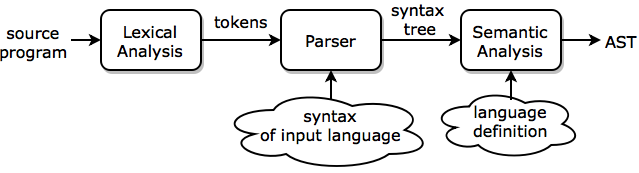
\includegraphics[width=\textwidth]{figures/frontend}%
\caption{Overview of the components that the frontend compromises.}
\label{fig:frontend}
\end{figure}

Listing \ref{lst:ir_code} shows an example C code where where we multiply two arguments and add them together to a third argument. On the right-hand part of this listing we can see the output that is generated by the front-end. Here we already have a notion of labels, similar to that of assembly code. The LLVM-IR code is in SSA form and consists of three-address operations. Here \emph{nsw} indicates that the result is undefined in case of an overflow.
%TODO BIG: add reference to 2.1, tell something about llvm's ir code representation, give examples, show phi node. 

\captionof{lstlisting}{Fragment of C code with corresponding LLVM-IR.}\label{lst:ir_code}
\begin{center}
\hspace{2px}\begin{minipage}{.475\textwidth}
\lstset{style=customc}
%\begin{lstlisting}[caption=List of instructions.,frame=tlrb]
\begin{lstlisting}[frame=tlrb]
int foo(int a, int b, int c)
{
  c += a*b;
  return c;
}

<@\ @>
\end{lstlisting}
\end{minipage}\hfill
\begin{minipage}{.475\textwidth}
\lstset{style=customasm}
%\begin{lstlisting}[caption=IR-code.,frame=tlrb]
\begin{lstlisting}[frame=tlrb]
define i32 @foo(i32 %a, i32 %b, 
                i32 %c) #0 {
entry:
  %mul = mul nsw i32 %b, %a
  %add = add nsw i32 %mul, %c
  ret i32 %add
}
\end{lstlisting}
%\vspace{1.9em}
\end{minipage}
\end{center}

% TODO: make graph to categorise optimizations on some criteria
\textbf{The optimizer} contains a collection of analysis and semantic-preserving transformations that can be used to optimize IR code. One of the advantages of LLVM is that when you build a new backend for any given processor architecture you immediately have access to all of these optimizations. Below we give some of these optimizations that are explained more detailed in the literature \cite[Chapter~9]{dragon_book}.%TODO: fix chapter in cite.
%TODO: add mem2reg
\begin{itemize}
\item \emph{Constant propagation:} computes for each point and each variable in the program, whether that variable has a unique constant value at that point. This can then be used to replace variable references with constant values.
\item \emph{Constant folding:} recognizes and evaluates constant expressions at compile time rather than runtime. For example, `$add\ 1+2$' can be replaced by `$3$'. Statements like `$add\ 1+2$' can be introduced by other optimizations, e.g. constant propagation. 
\item \emph{Common sub-expression elimination:} recognizes that the same expression appears in more than one place, and that performance can be improved by transforming the code such that the expression appears in one only place.
\item \emph{Copy propagation:} replaces each target of a copy statement with that of the copied value. For example, if we have a copy statement, $x = y$. Then the uses of $x$ can be replaced by $y$. Some optimizations require that this optimization is performed afterward to clean up, e.g. common sub-expression elimination requires this pass to run afterward. 
\item \emph{Dead code elimination:} removes code that does not affect the program's results. This avoids executing irrelevant operations and reduces the code size of a program.  
\item \emph{Loop invariant code motion:} aims at moving code that is independent of the loop iteration out of the loop body. It does this by moving the loop independent statement above the loop, saving it in a temporary variable, and use it in each iteration of the loop. Now the loop independent statement is computed only once instead of every iteration. 
\item \emph{Function inlining:} verifies whether inlining functions in its callees gives a performance benefit. If doing this would give a performance benefit, it replaces the call to the function with the function body. This optimization often is useful for small functions because it reduces the overhead that is introduced when a function call is made, e.g. storing frame pointer, storing function parameters and jump to the code to where the function is defined.     
\end{itemize}

\begin{figure}[b!]
\centering
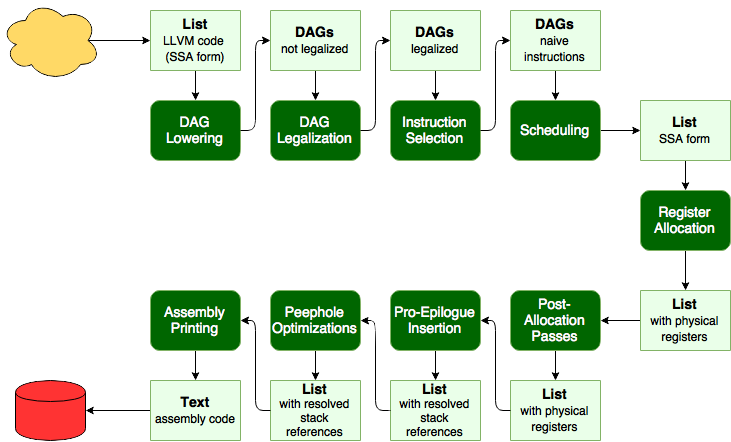
\includegraphics[width=\textwidth]{figures/code_generation_sequence}%
\caption{Code generation sequence, from LLVM code to assembly code.}
\label{fig:code_generation}
\end{figure}

%TODO: apply following namings: Instruction, Machine instruction, scheduled instruction in SSA form, schedule instruction not in SSA form.
\textbf{The backend} translates, according to a processor architecture, IR code to a target specific assembly language. It does this by going through a sequence of code generation stages, illustrated in Figure \ref{fig:code_generation}. The rectangular boxes indicate the data structure that is used by and produced by a given stage, and the name of each stage is denoted in a rectangular box with rounded corners. During this process, first, the IR code is lowered to a \emph{Directed Acyclic Graph} (DAG) in which each node represents an instruction. However, for some architectures, not all data types and instructions are supported. For this reason, the DAG is legalized to something that is supported by the target architecture. Instruction selection maps each of the nodes onto machine nodes, by matching patterns. %After that, the instruction selector maps the pattern of LLVM code into the target machine code and builds a new DAG whose nodes represents the target instructions.
Then we have a DAG consisting of only target specific machine instructions, in SSA form. Having naive machine instructions, the next step is to schedule them. We schedule the machine instructions according to the resource information of the target processor and assign each instruction to a specific cycle. 
%We will discuss scheduling in more detail in Chapter \ref{sec:scheduling}. 
Now the instructions are represented in a list rather than a DAG, but still in SSA form. The \emph{Register Allocator} (RA) then assigns physical registers to each of the virtual registers, now the list is not in SSA form. 
%We will discuss RA in more detail in Chapter \ref{sec:register_allocation}. 

The post-allocation pass can improve the schedule by taking physical registers and register pressure, that is known at this point, into account. After that, some epilogue and prologue code may be inserted, for example, saving/restoring the caller/callee registers and reserving/destroying of the function's stack frame. Peephole optimizations are target specific improvements to the generated code. These optimizations deal with very specific optimizations that can only be done at the end of the process. Finally, the assembly printer prints the generated code to a file.
%backend talk -> huuge



%\subsection{Instruction Scheduling}\label{sec:scheduling}
%After instruction selection, the program is represented in SSA form as a DAG. Each instruction is represented as a $MachineSDNode$ in a $MachineBasicBlock$. After scheduling has been performed, each instructions now is represented as a $MachineInstr$. 



%ach instruction is scheduleDuring instruction schdduling, each $MachineBasicBlock$ is scheduled by the scheduler and transformed into a $MachineInstr$. After this phase, instructions are represented as $MachineInstr$.

%\subsection{Register Allocation}\label{sec:register_allocation}
%Register allocation is executed during the code generation phase and consists of finding a mapping of a program with an unlimited number of virtual registers to a program with a limited number of physical registers.
%Examples, machine instrs on the left in SSA form, on the right with proper registers next to it.
%Introduce at least 

%TODO: 19 sept morning, Add examples of IR, CFG, Dominator tree ettc.
\subsection{Control Flow}\label{sec:control_flow_graph}
%\subsection{Representation of Code}
To analyze a code fragment, different representations can be explored. For instance, three-address IR code that is used by LLVM is conducive for further processing like optimizations and translations. Even further down the compilation line, we have assembly code, which is basically object code, but in human readable form. However, to analyze a fragment of code, we do not always need this much detail. Moreover, having this much detail, sometimes makes analysis more difficult. Control flow analysis is a code technique to analyze the control flow of a program. The control flow is expressed as a \emph{Control Flow Graph} (CFG), which is a more abstract representation of code that uses a graph notation to show all paths that can be traversed through a program during its execution.  
%TODO: Add cfg example with code left, cfg right

\begin{figure}[H]
\centering
\subfloat[C code fragment]{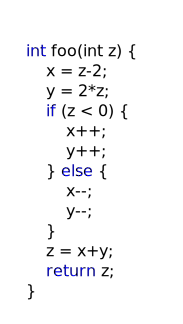
\includegraphics[width=.2\textwidth]{figures/cfg_fragment}%
\label{fig:cfg_fragment}}\quad\quad
\subfloat[CFG]{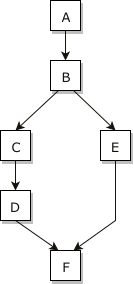
\includegraphics[width=.175\textwidth]{figures/cfg_fork_join}%
\label{fig:cfg_graph}}
\hfill
\caption{Example CFG with C code.}
\label{fig:cfg}
\end{figure}

In Figure \ref{fig:cfg_graph} we see a CFG for the code fragment in Figure \ref{fig:cfg_fragment}. In a CFG edges represent the control flow of the program and nodes represent basic blocks. A \emph{Basic Block} (BB) is a sequence of instructions with no branches, except for entering and leaving the basic block.
\\

%Another code representation that we would like to discuss here is a Dominator Tree (DomTree). Similar to a CFG, nodes represent BBs, but edges represent a dominator relationship. For two nodes $A$ and $B$, we say that $A$ dominates $B$, if all paths to $B$ go through $A$.

%TODO: add example CFG with corresponding DomTree

\subsection{Data Dependencies and Spilling}\label{sec:data_dependencies}
%\subsection{Scheduling Constraints}\label{sec:scheduling_and_ra}
%As we have seen above,
From a compilers perspective, certain operations address memory locations. A \emph{store} operation accesses the memory to put the value of a register into memory at a certain location, addressable by its address. On the other hand, \emph{load} operations load a value from memory at a certain location and puts that value in a register. These kind of operations are called memory operations. Other operations calculate a value and stores the result in a register. Operations that store the result in a register, or load a value from memory into a register, actually define that register. An example is given in the following code fragment:

%\lstset{style=customasm}
\begin{lstlisting}
lw  r2, r0, 4   # load from memory at location 0x4
lw  r3, r0, 5   # load from memory at location 0x5
mul r3, r3, r2  # define r3 with r3 = r3 * r3
sw  r3, r0, 2   # store result at location 0x2
\end{lstlisting}

Before scheduling and register allocation, the sequence of instructions contain an unlimited number of virtual registers and the instructions are in a DAG that preserves all control flow and data dependencies. Data dependencies are ordering constraints that influence the order of execution. Typically, there are three kinds of data dependencies \cite{data_dependece}:
\begin{enumerate}
\item There is a Read-after-Write (RaW) dependency, also called a \emph{flow dependency} from operation $a$ to operation $b$ if $a$ defines a register that may be used by $b$.
\item  There is a Write-after-Read (WaR) dependency, also called an \emph{anti-dependency} if for operations $a$ and $b$ when $a$ uses a register that is redefined by $b$. 
\item There is a Write-after-Write (WaW) dependency, or \emph{output dependency} from operation $a$ to operation $b$, if $a$ defines a register that is redefined by $b$.
\end{enumerate} 

Flow dependencies are also known as \emph{true dependencies} and anti and output dependencies as \emph{false dependencies}, introduced by scheduling or register allocation. While in SSA form, each variable is defined exactly once, therefore, we have only true dependencies in that form. After scheduling and register allocation, where we assign physical registers to each virtual register, we may assign one physical register to multiple virtual registers, which is illustrated in Listing \ref{lst:ra_example}. This process introduces false dependencies and can often be resolved with renaming techniques \cite{tta_codegen,renaming}.

\captionof{lstlisting}{Redefining physical registers by assigning them to multiple virtual registers.}
\begin{center}
%TODO: include a data dependency graph for the example below
\hspace{2px}\begin{minipage}[t]{.475\textwidth}
\begin{lstlisting}[frame=tlrb]
mul %v1, %src1, %src2
add %v2, %1,    %sum
mul %v3, %src3, %src4
add %v4, %v2,   v3
\end{lstlisting}
\end{minipage}\hfill
\begin{minipage}[t]{.475\textwidth}
\begin{lstlisting}[frame=tlrb]
mul r1, r5, r6
add r2, r1, r21
mul <@\hspace{1px}\textcolor{red!70!black}{r1}\hspace{1px}@>, r7, r8  # redefines r1
add <@\hspace{1px}\textcolor{red!70!black}{r2}\hspace{1px}@>, r2, r1  # redefines r2
\end{lstlisting}
\end{minipage}
\label{lst:ra_example}
\end{center}

%\lstset{style=customasm}
%\begin{center}
%\begin{minipage}{\linewidth}
%      \centering
%      \begin{minipage}{0.45\linewidth}
%          \begin{lstlisting}[frame=tlrb]
%(a) lw  r2, r5, 4
%(b) lw  r3, r6, 6
%(c) mul r3, r3, r2
%(d) lw  r4, r7, 0
%(e) add r4, r3, r4
%(f) sw  r4, r11, 0
%\end{lstlisting}
%          \captionof{subfigure}{Assembly code}
%          \label{fig:ddg_fragment}
%      \end{minipage}
%      \begin{minipage}{0.45\linewidth}
%          \begin{figure}[H]
%          \centering
%              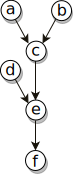
\includegraphics[width=.2\textwidth]{figures/ddg}%
%          \end{figure}
%          \captionof{subfigure}{DDG}
%          \label{fig:ddg_graph}
%      \end{minipage}
%\captionof{figure}{Example DDG with corresponding assembly code.}
%\label{fig:ddg}
%\end{minipage}
%\end{center}
%TODO: add more abstractions, also include dominator tree
Figure \ref{fig:ddg_graph} shows a data dependence graph corresponding to the code fragment in Figure \ref{fig:ddg_fragment}. In a data dependence graph nodes represent operations and the edges correspond to data dependencies.

%========= Store listing box =====
\newsavebox{\ddgfragmentlst}
\begin{lrbox}{\ddgfragmentlst}
  \begin{lstlisting}
(a) lw  r2, r5,  4
(b) lw  r3, r6,  6
(c) mul r3, r3, r2
(d) lw  r4, r7,  0
(e) add r4, r3, r4
(f) sw  r4, r11, 0
  \end{lstlisting}
\end{lrbox}

\begin{figure}[H]
  \centering
  \subfloat[Assembly fragment]{%
%    \usebox{\ddgfragmentlst}\label{fig:ddg_fragment}
   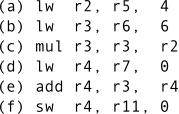
\includegraphics[width=.25\textwidth]{figures/ddg_fragment}\label{fig:ddg_fragment}
  } \quad\quad%\hfill%\hspace{35px}
  \subfloat[DDG]{%
   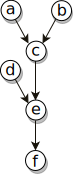
\includegraphics[width=.1\textwidth]{figures/ddg}\label{fig:ddg_graph}
  }
  \caption{Example DDG with corresponding assembly code.}
  \label{fig:ddg}
\end{figure}


%new TODO: add live interval analysis information or theory!!!
%TODO: add sentence in between
Sometimes there are not enough registers available to allocate physical rezgisters to all virtual registers because there are only a limited number of physical registers available. When the compiler runs out of registers to allocate, \emph{spilling} may be necessary to free one or more registers by storing them on the stack. Consequently, it is required to retrieve them from the stack just before they are used.

%TODO: add illustration of spilling?

%todo add theory, graph coloring on ddg graph.


%TODO: add control flow dependecy explanation, optionally from Code Generation for TTAs p.
%TODO: play with widths to get nicely in teh middle of the page.
%\lstset{style=customc}
%\begin{center}
%\begin{minipage}{\linewidth}
%\centering
%\begin{minipage}{0.2\linewidth}
%\begin{lstlisting}
%
%int foo(int z) {
%  x = z-2;
%  y = 2*z;
%  if (z < 0) {
%    x++;
%    y++;
%  } else {
%    x--;
%    y--;
%  }
%  z = x+y;
%  return z;
%}
%\end{lstlisting}
%\end{minipage}
%\hspace{0.05\linewidth}
%\begin{minipage}{0.4\linewidth}
%\begin{figure}[H]
%\centering
%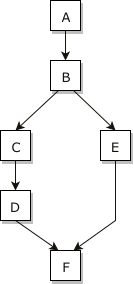
\includegraphics[width=.35\textwidth]{figures/cfg_fork_join}%
%\end{figure}
%\end{minipage}
%\captionof{figure}{A fragment of C code with a CFG.}
%\label{fig:cfg}
%\end{minipage}
%\end{center}

%TODO: insert general RA algorithms and heuristics. Graph colouring, and use this reference \cite{ra}.
%There are multiple register allocators available in LLVM, e.g. basic, fast, greedy and Partitioned Boolean Quadratic Problem (PBQP) register allocation. PBQP is a nearly optimal approach that does register allocation in phases, i.e. spilling, register assignment and copy coalescing. After spilling, RA can be done in polynomial time, but copy coalescing is NP-complete \cite{pbqp}. The other three register allocators are linear scan based algorithms that use heuristics and visit live ranges in order, although it is possible to implement a custom register allocator.
%TODO: decide to add or not to add.

%TODO: insert scheduling talk, including algorithms, heuristics and LLVMs available schedulers.
%TODO: move to later.
%A common problem in compilers is the ordering in which to do scheduling and register allocation. If registers are allocated before scheduling, the resulting code tends to have many storage dependencies that limit code scheduling. On the other hand, if the code is scheduled before register allocation, the schedule created may require so many registers that register spilling is required, which may negate the advantages of instruction-level parallelism (ILP) \cite[Chapter~10.2.4]{dragon_book}. Whether to do register allocation first, or scheduling first, or to address these problems at the same time is often referred to as, phase-ordering problem. 

%In general, you can solve scheduling exactly using algorithms, e.g. integer programming or constraint programming, or one can solve the problem, but without guaranteeing that an optimal solution is found using heuristics. With LLVM there are two main schedulers, i.e. list scheduler and Machine Instruction (MI) scheduler that use heuristics to find a solution, although it is possible to implement a custom scheduler for an architecture at hand. 

%TODO: add basic introduction to bypassing, from presentation.

\newpage
\section{Explicit Datapaths}\label{sec:datapaths}
Data goes through a particular path through the pipeline of a processor and typically, a pipeline is split up in multiple stages. With a lockstep processor, each of the stages are effectively working in parallel. Figure \ref{fig:pipelining} illustrates hardware pipelining for a \emph{Reduced Instruction Set Computer} (RISC) processor. The pipeline is split up in four or more stages, e.g. instruction fetch, instruction decode, execution and write-back stage. During the \emph{instruction fetch} (IF stage) an instruction is loaded from \emph{instruction memory} (IMEM), which is decoded in the \emph{instruction decode} (ID) stage where the type of operation is determined by the opcode and operands are identified by their register addressing, and finally, the operation is executed and the result is written back to the register file.

\begin{figure}[H]
\centering
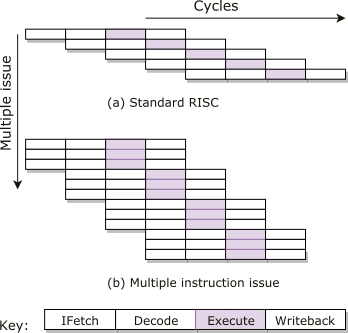
\includegraphics[width=.5\textwidth]{figures/pipelining}
\caption{Pipelining and multiple instruction issue\cite{tta_codegen}.}
\label{fig:pipelining}
\end{figure}

\begin{figure}[b]
\centering
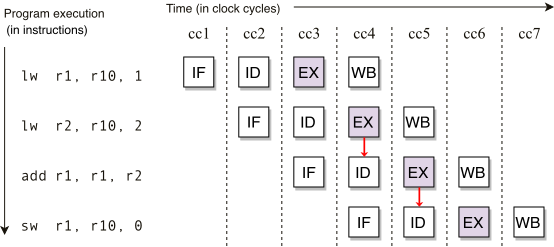
\includegraphics[width=.8\textwidth]{figures/bypassing_example}
\caption{Instructions being executed using the single-cycle datapath, assuming pipelined execution.}
\label{fig:bypass_problem}
\end{figure}

\textbf{Operand forwarding:} When bypassing is completely absent the result of an instruction can only be obtained after it is written back. On the other hand, with bypassing, a bypass network of wires and busses connects the execution and writeback stages back to the ID stage. We may forward a value using these wires or busses to operands of another instruction. This way, we can obtain the result of an instruction before it has been written back to the register file. We illustrate this behaviour in Figure \ref{fig:bypass_problem}.

Four consecutive instructions are executed of which the last two instructions have a RaW dependency with the instruction prior to it. As you can see in Figure \ref{fig:bypass_problem} the instructions prior to said instructions are in the execution stage when their result is required, namely, when said instructions are in the ID stage. We either need to stall for a cycle, such that the previous instruction is in the WB stage, or we need to forward the result from the execution stage to the ID stage. Since insertion of stall cycles results in less efficient code, we choose to forward the result using the bypass network (indicated with a vertical arrow from EX to ID).

%TODO: update picture, make nicer and have on top stages, and below remain almost the same
%\begin{figure}[H]
%\centering
%\subfloat{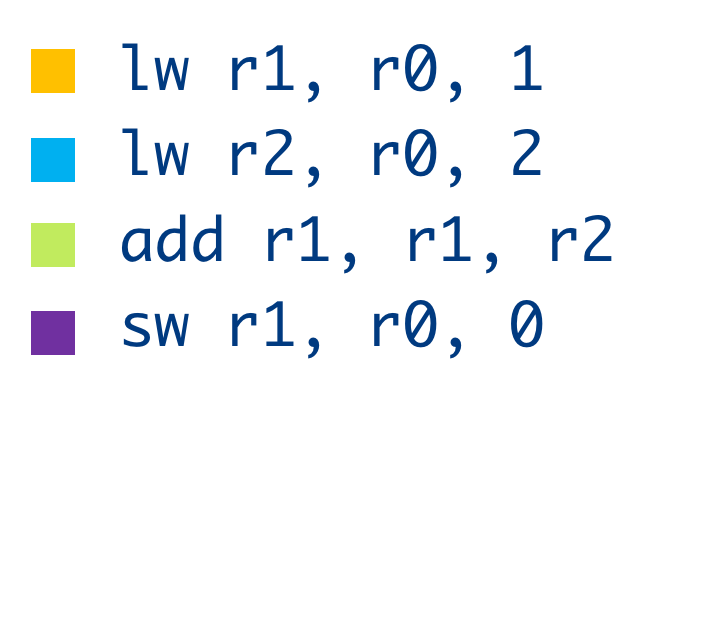
\includegraphics[width=.275\textwidth]{figures/bypass_prob_legend}}
%\hfil
%\subfloat{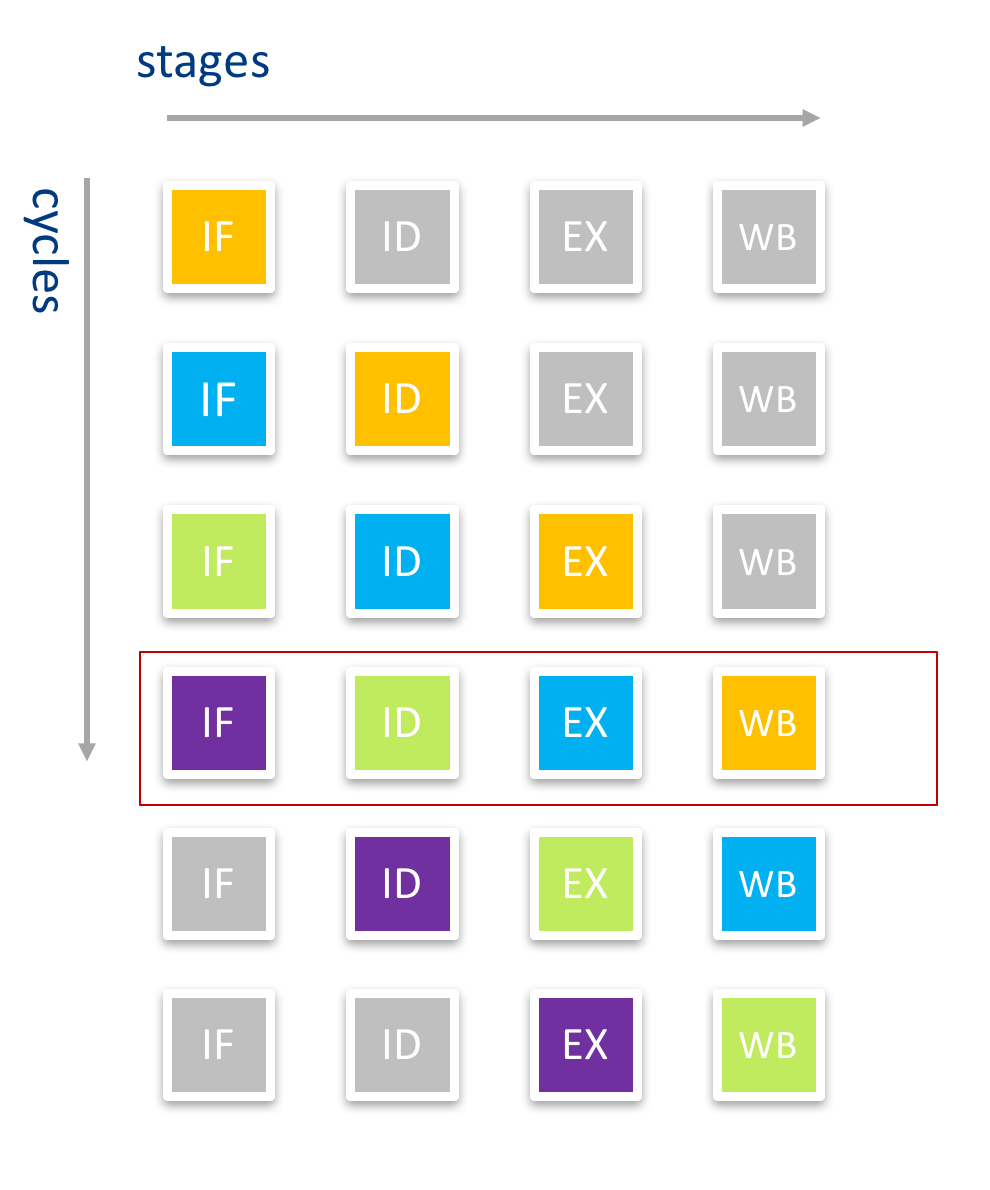
\includegraphics[width=.475\textwidth]{figures/bypass_problem}}
%\caption{Bypassing network differences between four stage and five stage pipeline configuration.}
%\label{fig:bypass_problem}
%\end{figure}
%TODO: replace with picture from presentation (03_nov)
\subsubsection{Implicit Datapaths}
With implicit bypassing (also called transparent bypassing), bypassing opportunities are detected and controlled by dedicated hardware on chip. However, doing this at run-time has some advantages and some disadvantages.
\begin{itemize}
  \item\textbf{Advantage:} 
    With bypassing, operand forwarding is possible which reduces the number of reads from the register file. This will reduce register file usage and may improve energy efficiency of the processor.
  \item\textbf{Disadvantage:} 
    If you push the responsibility of identifying and exploiting forwarding to the hardware, it needs $2\cdot d\cdot n$ comparators (where $d$ is the number of stages between ID en WB and $n$ the number of issue slots) to compare operands of an instruction to registers defined by previous instructions that are already in the pipeline. Altogether, this results in a more complex gate design and increased area.
\end{itemize}

It has been observed that variables in the register file are often transient, meaning that they last only for a short time.  Reads from the register file of said variables can be avoided by forwarding which we showed in the previous paragraphs.\\

We now show that we can avoid writes of transient values to register with explicit datapaths. The reason why this is only the case for explicit datapaths, and not with implicit bypassing, is that the hardware can only look at instructions that have already been executed, while the compiler can look at all instructions of a program.\\

\textbf{Dead result elimination:} 
If all consumers of a variable obtain it using forwarding, then it will never be read from the register file. Therefore, we do not need to store it anymore in a register file and we can avoid these obsolete stores.  

\subsubsection{Explicit Datapaths}
With explicit datapaths (sometimes referred to as exposed datapaths), bypass opportunities are detected and controlled by the compiler. Doing this at compile time rather than run-time has some advantages and some disadvantages.
\begin{itemize}
  \item\textbf{Advantage:}
    With explicit bypassing, dead result eliminations is possible which reduces the number of writes to the register file. This will further reduce register file usage and may further improve energy efficiency of the processor.
  \item\textbf{Disadvantage:}
    The compiler needs to take datapaths and variables that are in the pipeline into consideration, because bypassing is explicit in the compiler. This results in a more complex compiler.
\end{itemize}



\newpage
\section{SIMD Processor Architecture}\label{sec:simd}
%TODO: rewrite
%TODO: reduce total number of todos
%TODO: add paragraph about xetal-pro from preparation

\begin{figure}[t]
\centering
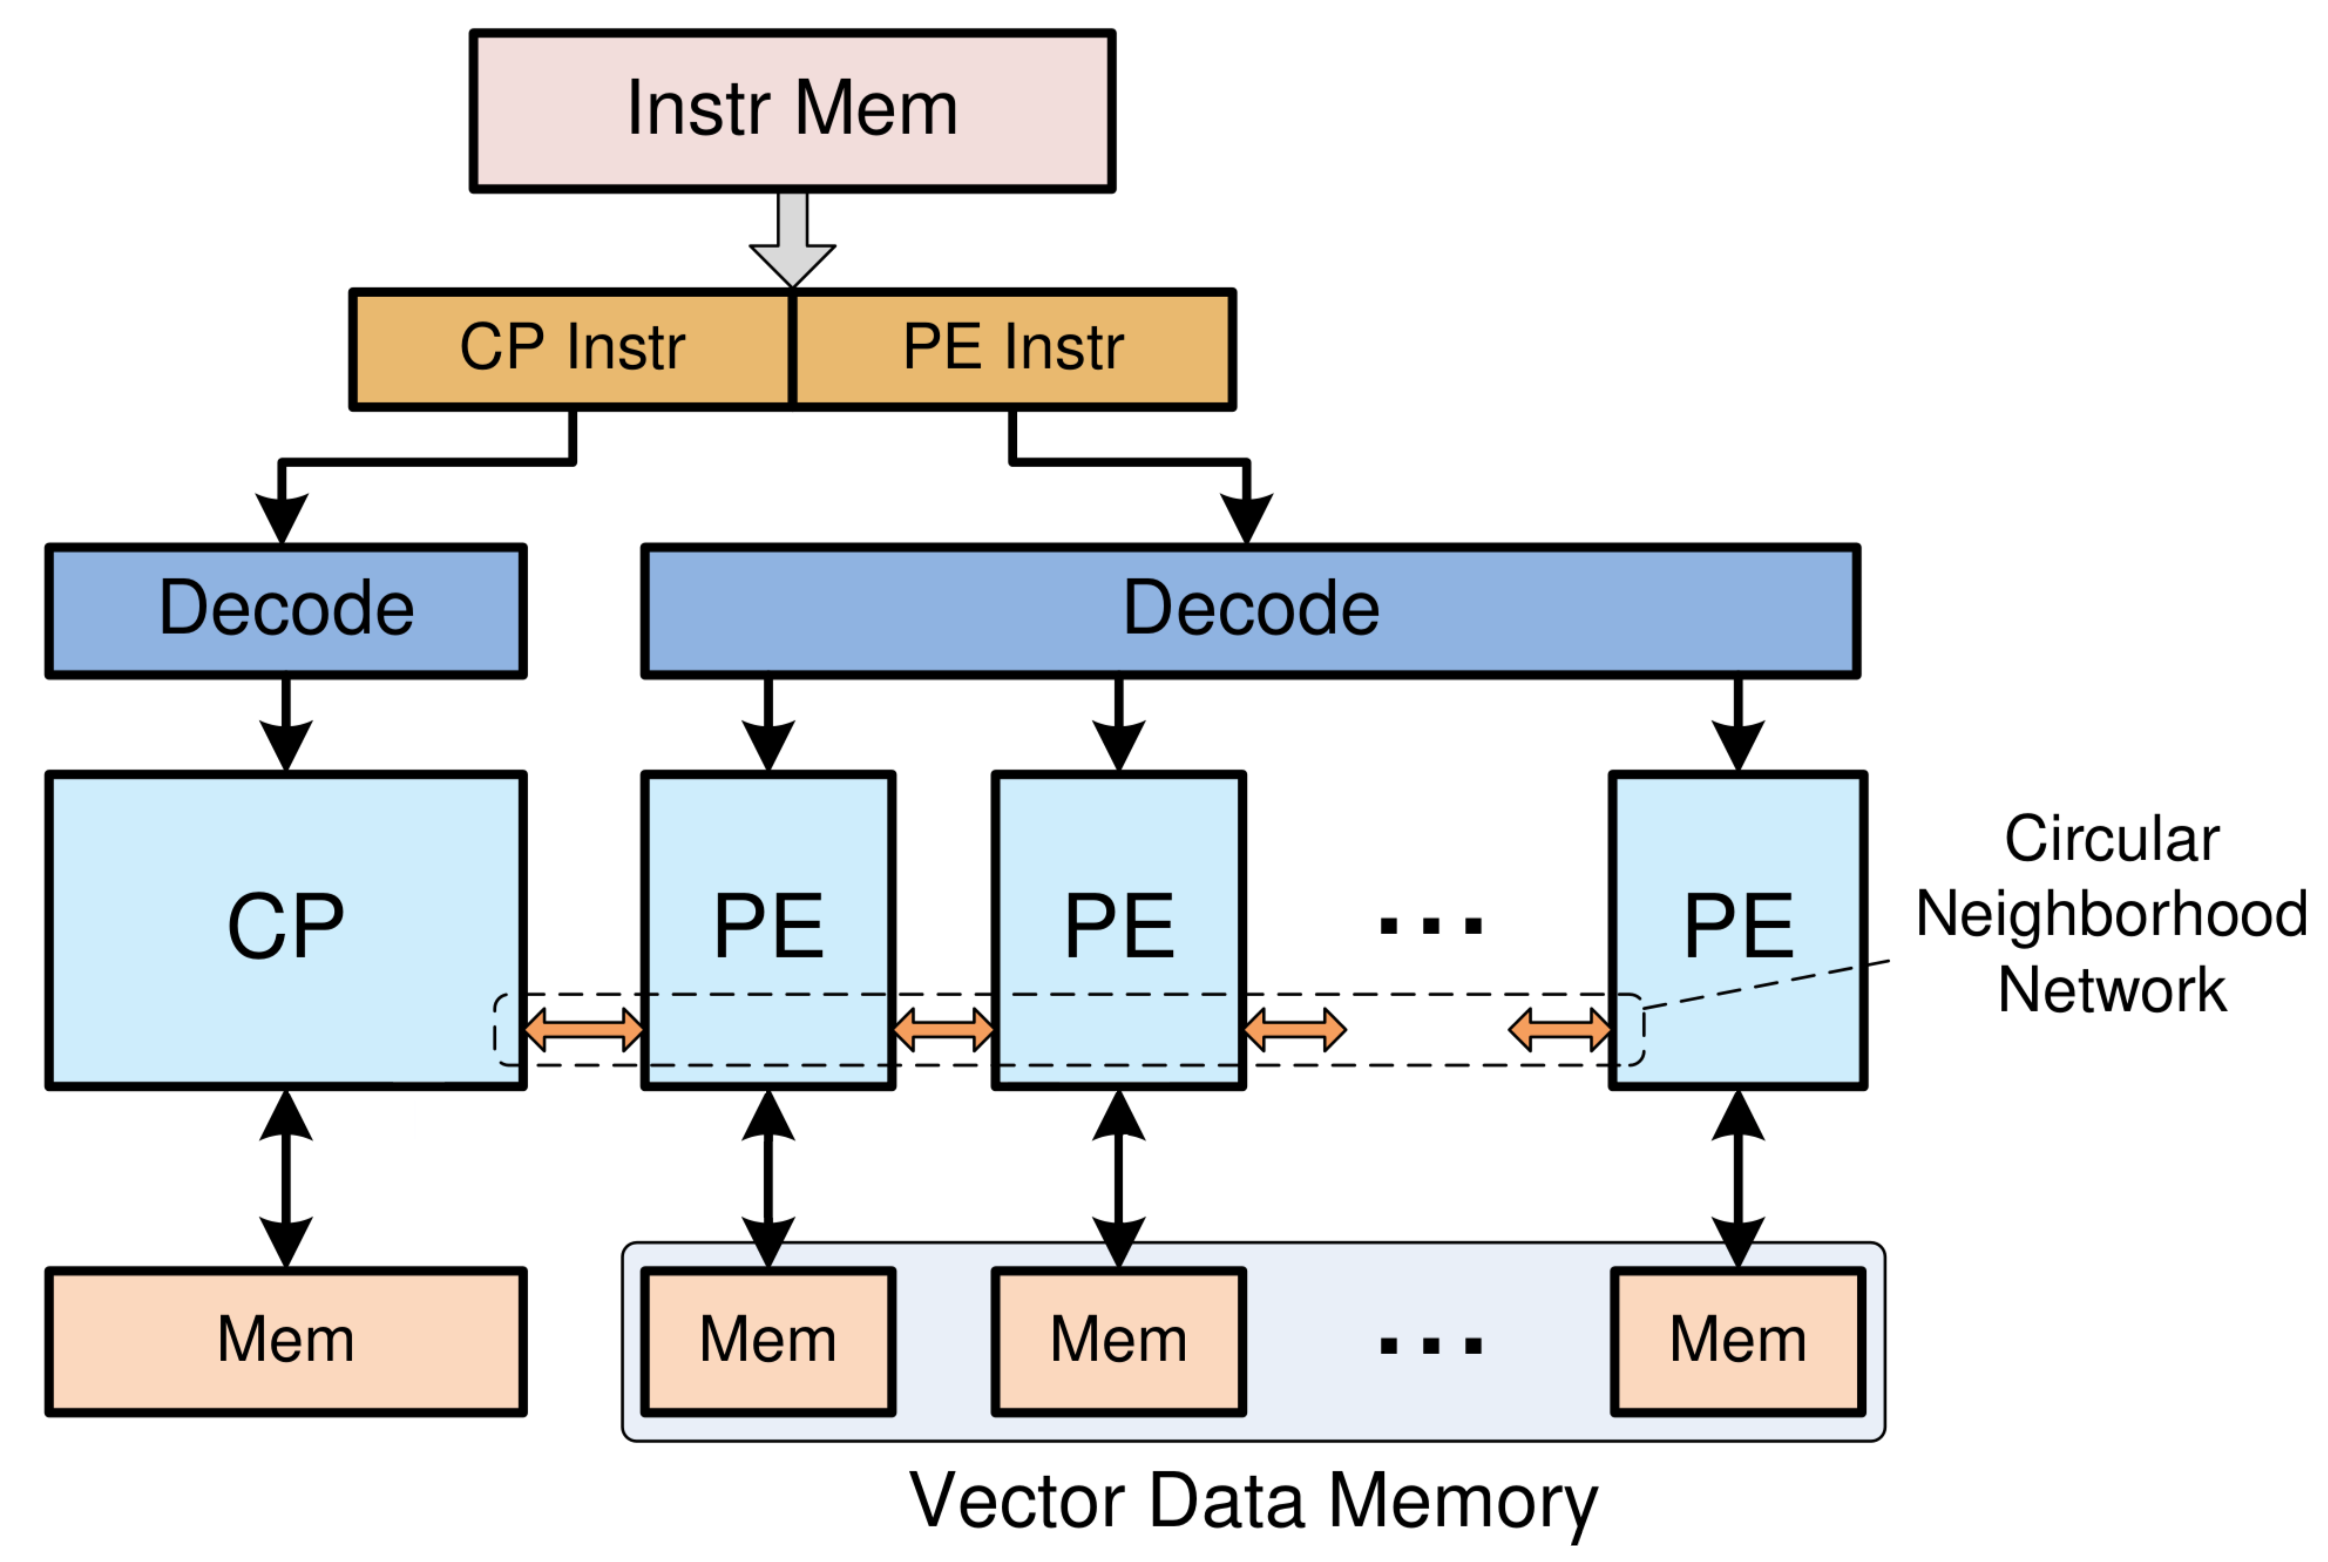
\includegraphics[width=.6\textwidth]{figures/simd_overview}
\caption{General overview of the wide SIMD architecture.}
\label{fig:simd_overview}
\end{figure}

The advantage of the SIMD architecture is that multiple operations are processed in parallel instead of processing them in a sequence. Therefore, the same performance can be achieved at a much lower clock frequency, thereby reducing voltage and thus energy consumption \cite{dongrio1}. Furthermore, because each Processing Element (PE) executes the same instruction, the Instruction Fetch (IF) and Instruction Decode (ID) can be shared amongst the PEs, reducing energy consumption.

We propose a wide SIMD architecture \cite{simd} that performs wide vector operations that exploit DLP by executing the same instruction on multiple data simultaneously. Figure \ref{fig:simd_overview} shows a general overview of the SIMD processor.
We have one Control Processor (CP) responsible for scalar operations and control flow i.e. jump/branch instructions. Furthermore, there is a wide array of PEs responsible for processing vector operations. The CP executes in parallel with the PEs, exploiting ILP.

The proposed architecture has a Reduced Instruction Set Computer (RISC) Instruction Set Architecture (ISA) that is divided up into three categories of instructions. In general, instructions have two operands and a destination register. Instructions that take two register files as operands are Register-type (R-type) instructions. Instructions that take a register file and an immediate as operands are called Immediate-type (I-type). The control flow can be controlled by using Jump-type (J-type) instructions, which can only be executed by the CP.

\begin{figure}[b!]
\centering
\subfloat[Datapath with implicit bypassing.]{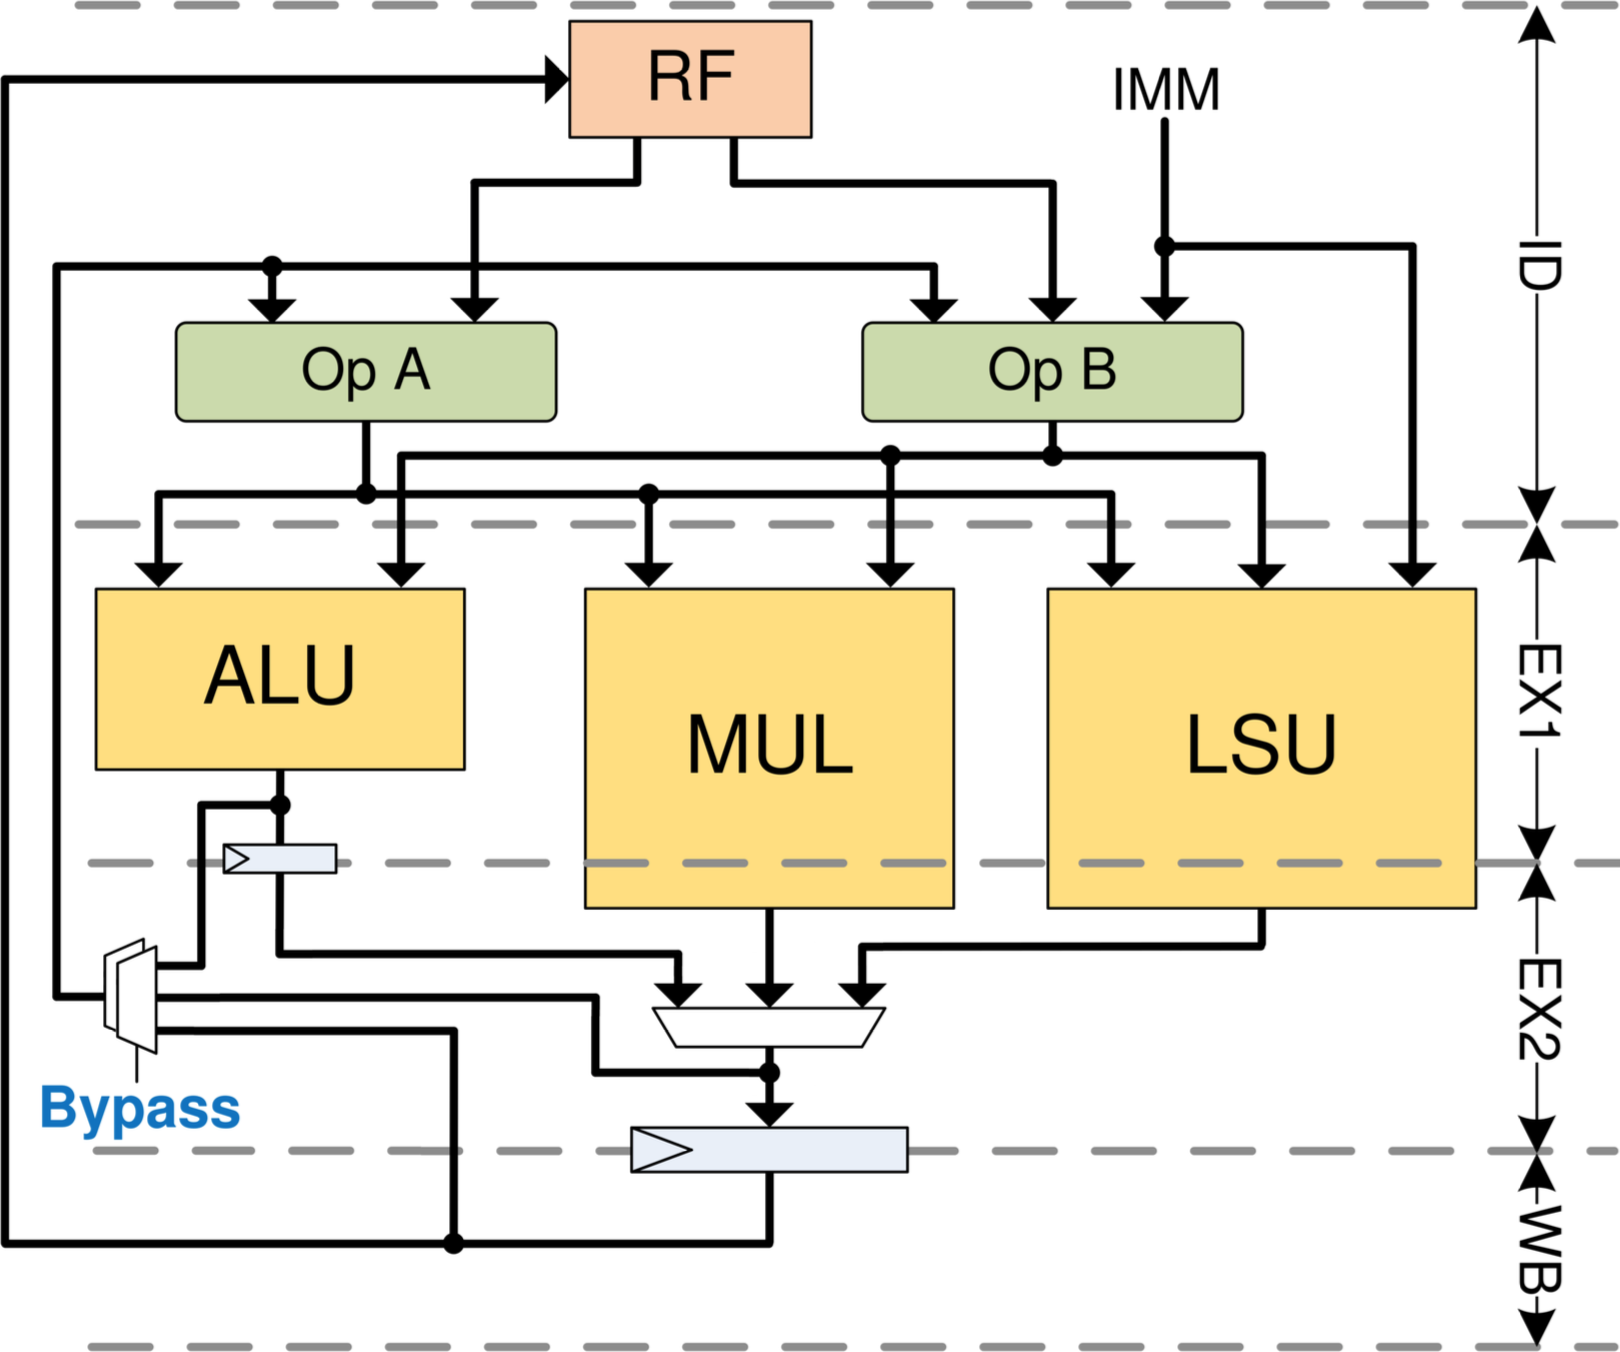
\includegraphics[width=.475\textwidth]{figures/transparent_bypass}%
\label{fig:transparent_datapath}}
\hfil
\subfloat[Datapath with explicit bypassing.]{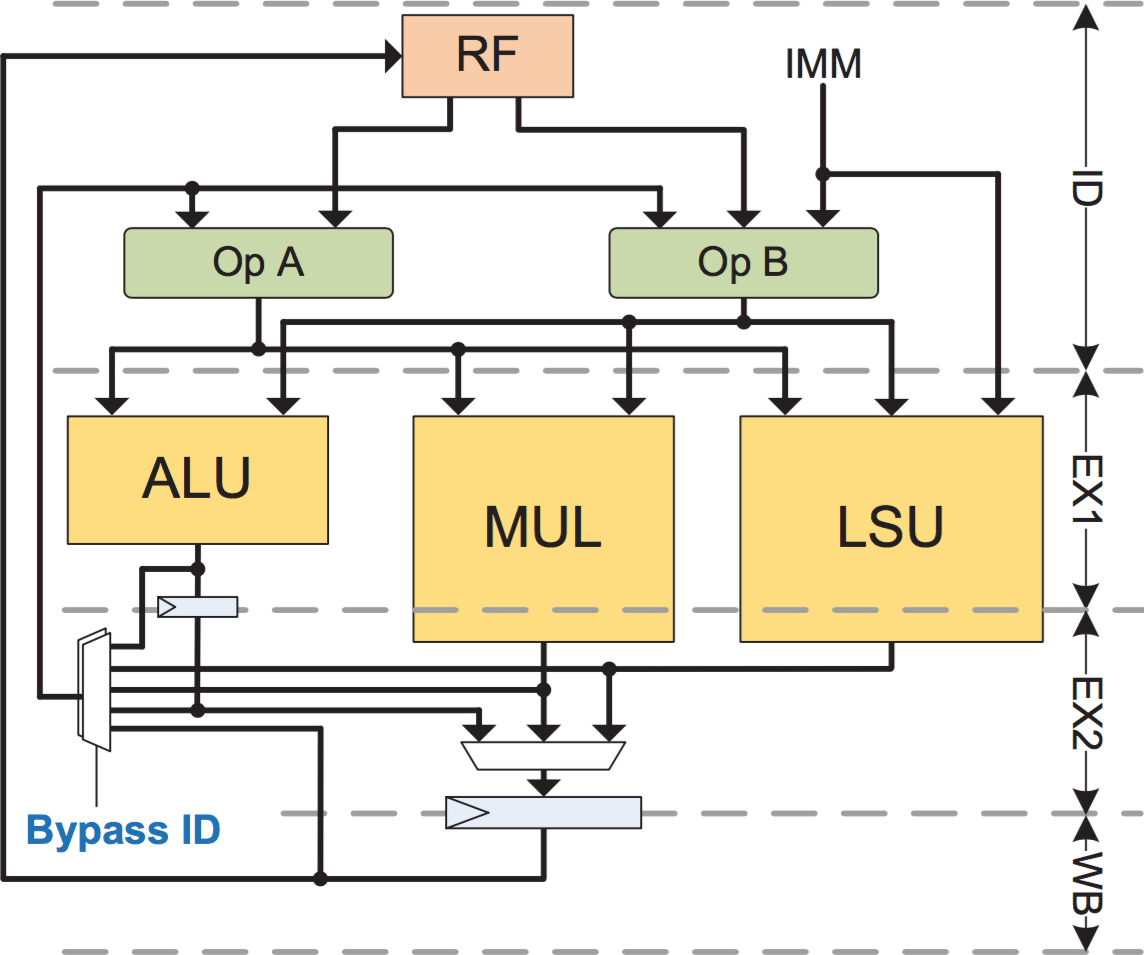
\includegraphics[width=.475\textwidth]{figures/explicit_bypass}%
\label{fig:explicit_datapath}}
\caption{Bypassing network differences between implicit bypassing and explicit bypassing.}
\label{fig:datapath_approaches}
\end{figure}

%TODO: add here that we have in general an iF, ID, one or more EX and a wb stages and that normally the result is not available until after the wb stageis complete, but with bypassing, whether it is transparent or explicit bypassing, we can get the result at an earlier stage. 

As an extra challenge for the compiler, the architecture is designed to be configurable, e.g. width of the PE array, bit width of the wires and registers, the number of stages that the instruction pipeline consists of, and whether it has implicit or explicit bypassing, can be configured. The data width of the wires and registers can be configured into 16-bits or 32-bits.

In order to support a configurable number of PE elements, a neighbourhood network topology is chosen for its scalability. With a circular neighbourhood network topology, the connection between the first and last PE does not introduce extra long wires, because the PEs can be placed in a circular manner \cite{dongrio2}.

%=============================== NN speech ===============================
%\section{Neighbourhood Network}\label{sec:nn}
%Each processor (CP or PE) does not only execute independently, but can also exchange data with its direct neighbours. However, because we have limited connectivity, moving data from one PE to another PE can introduce additional cycles. Namely, when communicating with non-direct neighbours. The circular neighbourhood network that is used to connect the processors is illustrated in Figure \ref{fig:neighborhood_network}. The CP can select data from the first and last PE, and each PE can communicate with its direct neighbours, or (not illustrated in Figure \ref{fig:neighborhood_network}) receive data from the CP by means of a broadcast.

%\begin{figure}[H]
%\centering
%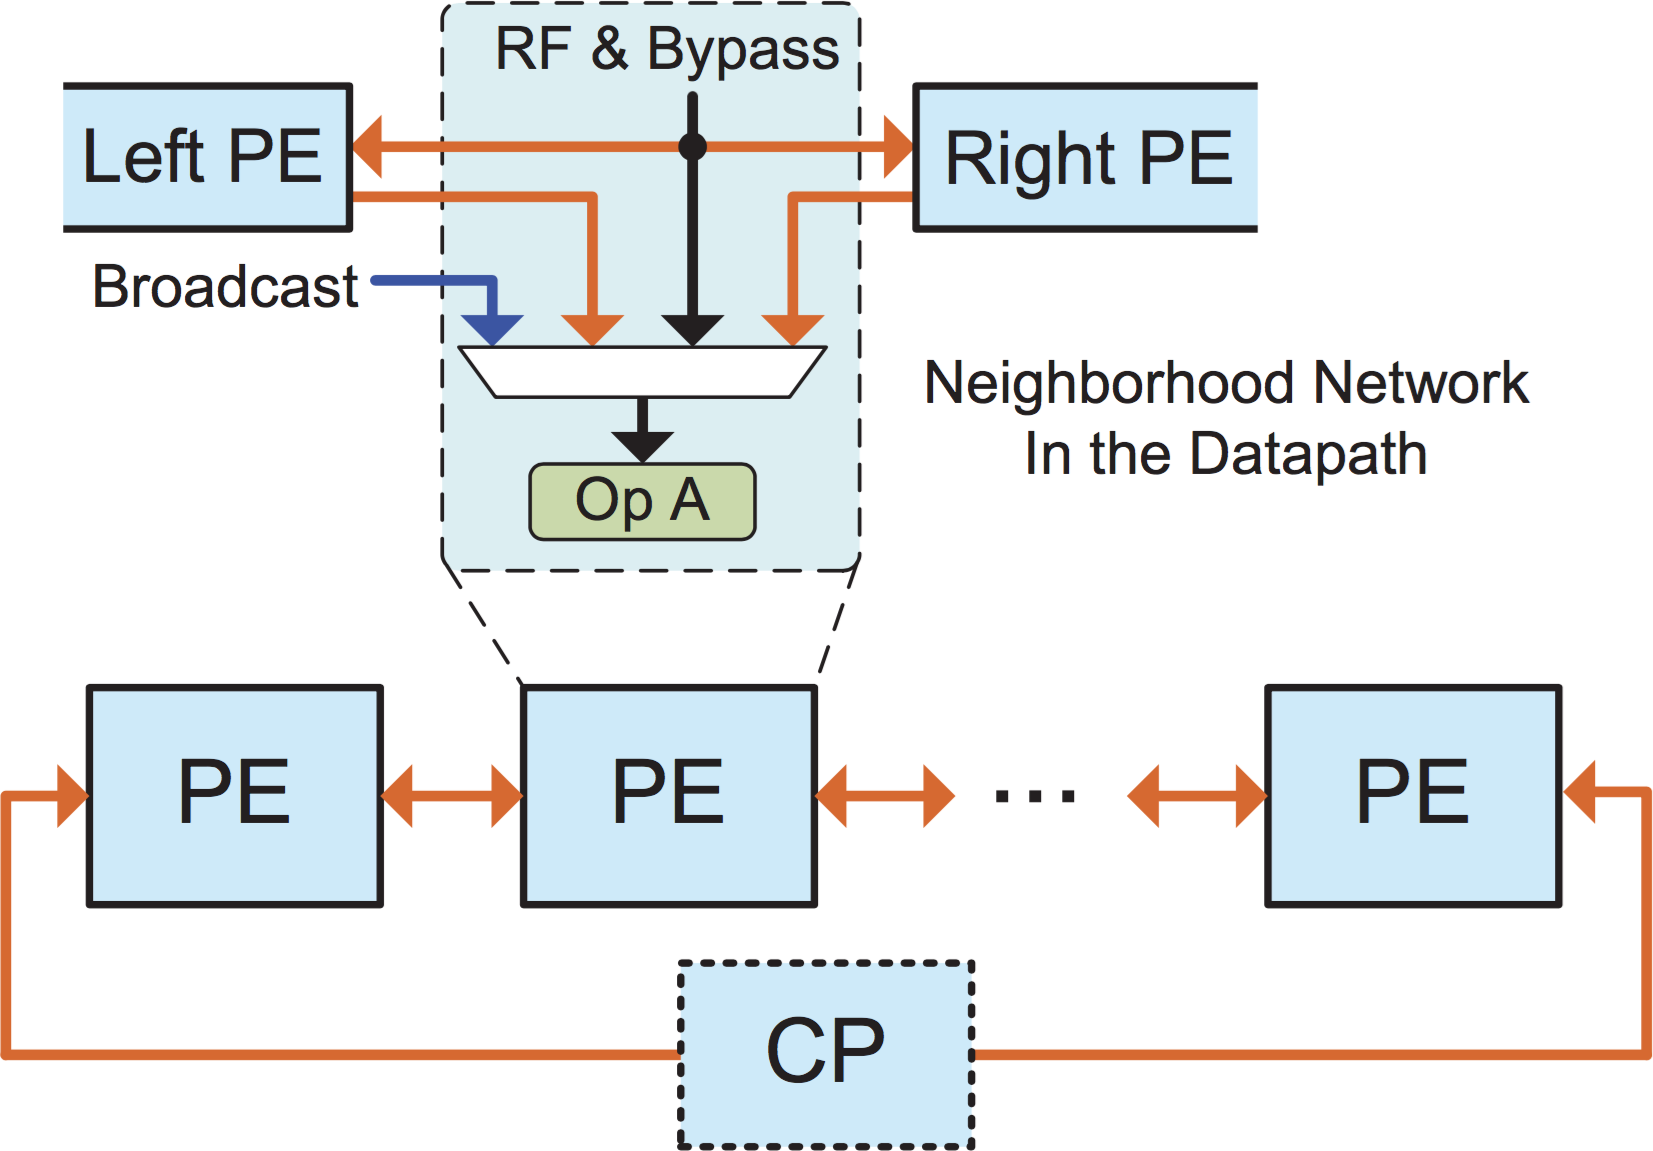
\includegraphics[width=.4\textwidth]{figures/neighborhood_network}
%\caption{Illustration of the circular neighborhood network.}
%\label{fig:neighborhood_network}
%\end{figure}

%The processor selects data from its neighbours in the instruction decode stage. Depending on the "select data" bits, it either takes data from one of its neighbours or from itself. Table \ref{table:select_data} gives an overview of the communication mode, depending on the value of "select data". The "select data" bits are decoded in each instruction, as we will show in Chapter \ref{sec:isa}.
 
% \begin{table}[H]
%\caption{Communication model for the CP and PEs, depending on the value of "select data".}
%\begin{center}
%\begin{tabular}{|c|c|c|}
%\hline
%\textbf{select data} & \textbf{CP} & \textbf{PE} \\ \hline
%2'b00 & Select data from \emph{self}. & Select data from \emph{self}. \\ \hline
%2'b01 & Select data form \emph{last} PE. & Select data from \emph{right} neighbour. \\ \hline
%2'b10 & Select data from \emph{first} PE. & Select data from \emph{left} neighbour. \\ \hline
%2'b11 & Not used. & Select data from CP \emph{broadcast}. \\ \hline
%\end{tabular}
%\end{center}
%\label{table:select_data}
%\end{table}%

%The processors communicate with each other by writing directly to the output of the operand register based on the values of bits "select data" bits. When the value of these two bits is $00$, data is selected from the processor itself. When these bits are $01$, data is selected from the last PE, in case of the CP executing this instruction, and from the right neighbour in case of a PE executing this instruction. Similarly, having a value of $10$, data is selected from the first PE in case of the CP executing this instruction, or left neighbour in case of a PE is executing this instruction. Finally, a value of $11$ will select data from the CP broadcast in the case that a PE is executing the instruction.

%=============================== Datapath speech ===============================
\subsection{Processor Pipeline and Datapath}\label{sec:processor}
%TODO: make new pictures for difference 4 and 5 stage without all difficult information
\begin{figure}[b!]
\centering
\subfloat[4-stage pipeline processor overview.]{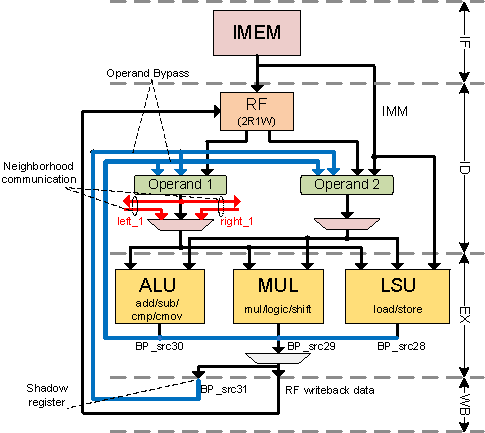
\includegraphics[width=.475\textwidth]{figures/4-stage_bypass}%
\label{fig:4_stage}}
\hfil
\subfloat[5-stage pipeline with processor overview.]{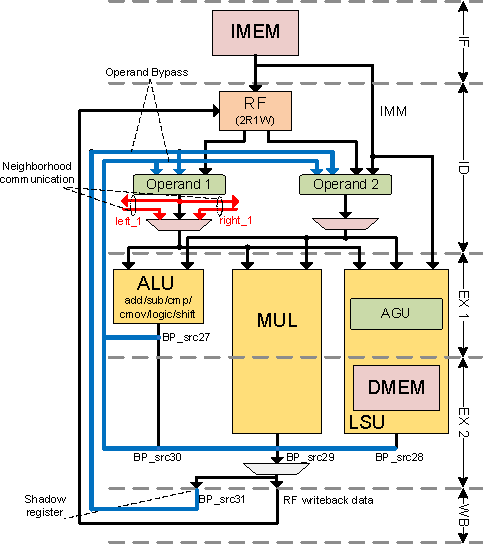
\includegraphics[width=.475\textwidth]{figures/5-stage_bypass}%
\label{fig:5_stage}}
\caption{Bypassing network differences between four stage and five stage pipeline configuration.}
\label{fig:datapath_pipeline_conf}
\end{figure}
%TODO: Write new paragraph about.general layout

Generally, each processor (CP or PE) has its own registers and three functional units, i.e. ALU, MUL and LSU. 

The instruction pipeline is divided up into four or five stages. Top down, we have an IF-stage, an ID-stage, one or more execution stages and a Write Back (WB) stage. The architecture shown in Figure \ref{fig:4_stage} has four stages while the architecture shown in Figure \ref{fig:5_stage} has five stages.

The neighbourhood communication network is implemented by overriding the output of $operand\ 1$ in ID-stage. Depending on the decoded instruction, data is either selected from another (neighbouring) processor, from the local RF or from the bypass network. Each FU has private input registers, which keep the result at the output of a compute unit valid as long as no new operation or input is assigned to it \cite{dongrio1}. The outputs can be used in the bypass network to bypass any of the operands in an instruction. This \emph{operand isolation} reduces toggling in the FUs, and creates extra opportunities for bypassing.

We can configure the SIMD to have either explicit or implicit bypassing. With implicit bypassing, also called transparent bypassing it is the hardware's responsibility to handle bypassing. With explicit bypassing, on the other hand, the bypasses are encoded in the instructions, and it is thus the compiler's responsibility to handle bypassing.

%We can configure the SIMD to have four or five stages. With four stages shown in Figure \ref{fig:4_stage}, all instructions take a single cycle, while with the five stages shown in Figure \ref{fig:5_stage}, ALU takes a single cycle, while MUL and LSU take two cycles, as shown in Table \ref{table:FU_cycles}. With 5 stages, MUL takes twice as many cycles. However, additions are simpler to perform, therefore the efficiency. 

%\begin{table}[H]
%\caption{Cycles per FU.}
%\begin{center}
%\begin{tabular}{|c|c|c|}
%\hline & \multicolumn{2}{c|}{\textbf{Cycles}} \\ \hline
%\textbf{FU} & \textbf{4-stage} & \textbf{5-stage} \\ \hline
%ALU & 1 & 1 \\ \hline
%MUL & 1 & 2 \\ \hline
%LSU & 1 & 2 \\ \hline
%\end{tabular}
%\end{center}
%\label{table:FU_cycles}
%\end{table}%

%The main difference between the two approaches is that where transparent bypassing always performs a write to a register, this is optional for explicit bypassing, as we will show in Chapter \ref{chapter:software_bypassing}.
One of the advantages of explicit bypassing is that certain writes to a register can be avoided. Namely, when the result of an instruction is bypassed and not used anywhere else, we do not need to store it in a register because we would never read it. Avoiding writes to the RF reduces the total energy consumption. Since there are many register files in a wide SIMD, reducing the energy consumption of the register file has a large impact on the overall energy consumption \cite{dongrio1}. Because of this, reducing the register file's energy consumption is of great importance. Furthermore, the explicit data path shown in Figure \ref{fig:explicit_datapath} has two extra sources compared to the transparent data path in Figure \ref{fig:transparent_datapath}. These additional bypass sources increase the chance that a result is being bypassed. In the explicit bypassing version, bypassing sources are directly accessible by the instruction. This is done by reserving part of the RF address space for the bypass sources. The disadvantage of this is that the register index space is reduced, however, we do not have to change the instruction format in order to specify that an operand of an instruction is bypassed from a previous instruction.

The total number of registers grows linearly with the number of PEs because each processor has 32 registers. With a wide SIMD, we, therefore have many registers that in total consume a considerable amount of energy, namely 34.6\% of the total energy consumption \cite{dongrio1}.

%Todo: change this picture to have explicit and implicit bypassing instead. State then that we will be focussing on explicit bypasisng.



%Todo: add small example, having on one side normal ops. On the other hand haing implicit bypassing and finally explicit bypassing (without the store).

%\begin{figure}[b!]
%\centering
%\subfloat[4-stage pipeline with explicit datapaths.]{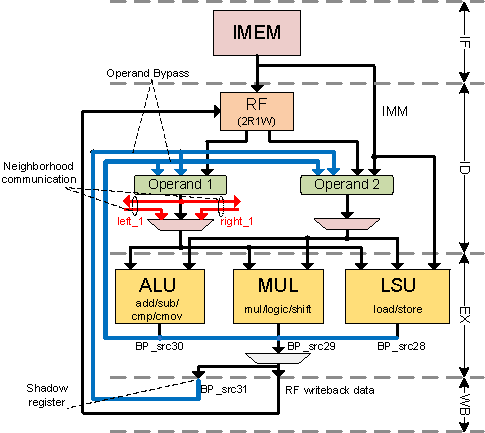
\includegraphics[width=.4\textwidth]{figures/4-stage_bypass}%
%\label{fig:4stage}}
%\hfil
%\subfloat[5-stage pipeline with explicit datapaths.]{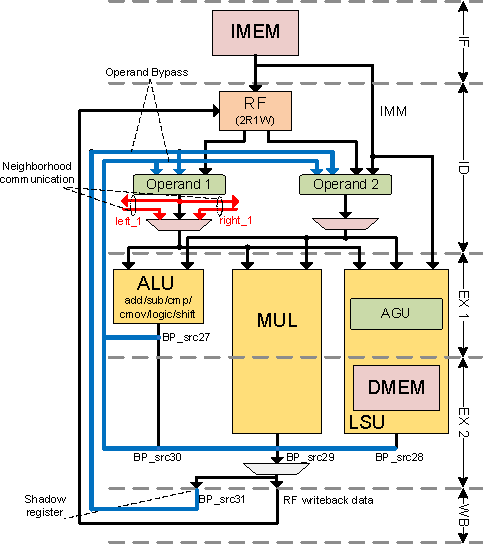
\includegraphics[width=.34\textwidth]{figures/5-stage_bypass}%
%\label{fig:5stage}}
%\caption{The pipeline of the SMD processor architecture with explicit datapaths.}
%\label{fig:pipeline_stages}
%\end{figure}

%%=============================== instruction format speech ===============================
%\section{Instruction Format}\label{sec:isa}
%%Change (optional)
%%% namely, one scalar and one vector instruction.
%%With
%%% namely, one scalar instruction that is executed on the CP, and one vector instruction that is executed on each of the PEs.
%Similar to a 2-issue VLIW instruction, an SIMD instruction consists of two subinstructions. An SIMD instruction is a 56-bit instruction that is divided up in two 28-bit subinstructions, namely, a scalar and a vector instruction. Only the CP can perform jump and branch instructions, therefore, the vector instruction can be either a R-type or an I-type instruction, while a scalar instruction can be a R-type, I-type or J-type instruction. Both sub instructions have a format, as shown in Figure \ref{fig:instruction_format}.

%\begin{figure}[H]
%\centering
%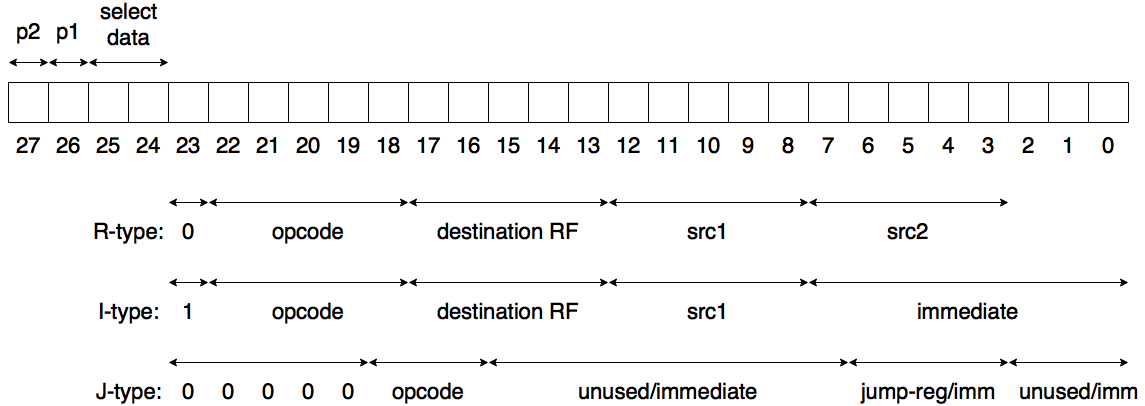
\includegraphics[width=\textwidth]{figures/instruction_format}
%\caption{Generic overview of the instruction format.}
%\label{fig:instruction_format}
%\end{figure}

%There are two guard bits $p1$ and $p2$, that can be set by using a set flag instruction. Consequently we can them for predicate execution. The instructions, branch if flag (not) set and conditional move read the predicate flag before executing. For the full overview of supported instructions, see Appendix \ref{chapter:supported_operations}.

%Note that the "select data" bits are also part of the instruction as we explained in Chapter \ref{sec:nn}. The CP and PEs can communicate by setting these bits. The communication model is shown in Table \ref{table:select_data}.

%TODO: elaborate delay slot, with link to explanation of pipelining.
%todo update extend rewrite

\section{Related Work}\label{sec:related_work}

% Other exposed or explicit datapath architectures and their corresponding compilers.

% Other pure SIMD architectures, GPU and its difference if i know this and can tell it.

% Liu's work on compiler design, and what it lacks, proper support for 5-stage configuration, explicit bypass conf. 

%Old rel. work
There is related work for compilers that target SIMD architectures, in particular, a compiler has been developed, referred to as legacy compiler. Furthermore, compiling with explicit datapaths has been an active research topic for other architectures.
% scrap
%The related work is introduced in this part, including the legacy compiler, building the LLVM back-end for SIMD architecture, explicit datapaths in other architecture and some scheduling and register allocation algorithms applied in other compilers.

%\section{Building an LLVM back-end}
%Our backend is derived from tricore tutorial on creating a new backend for the LLVM compiler framework \cite{tricore}. Furthermore, based on that work, an LLVM backend for SIMD architecture without explicit bypassing has been developed \cite{liu_zhenyuan}. However, the current compiler generates code with implicit bypassing. We, therefore, need to extend this to efficiently generate code for explicit bypassing as well. Therefore, our work will be an extension to previously noted work.

\subsection{Other Exposed/Explicit Datapath Architectures}\label{sec:other_explicit_datapaths}
Compiling with explicit datapaths has been an active topic of research. Several architectures that face similar challenges have been investigated. 

%Johan janssen & ... TTA work
%Other exposed datapaths

\subsubsection{Transport Triggered Architectures}\label{sec:tta}
One of the main works that was investigated is the  \emph{Transport Triggered Architecture} (TTA) which has been developed in the MOVE project \cite{tta_codegen}. For TTA architectures, instructions consist of transports that specify the datapath. The difference between TTAs and traditional operation triggered architectures is that TTA are transport driven, hence its name. 

Figure \ref{fig:tta} illustrates how function units and register files are connected to an interconnect network which are programmed by instructions. Programming a TTA consists of moving operands to the input registers of a FU.

\begin{figure}[b!]
\centering
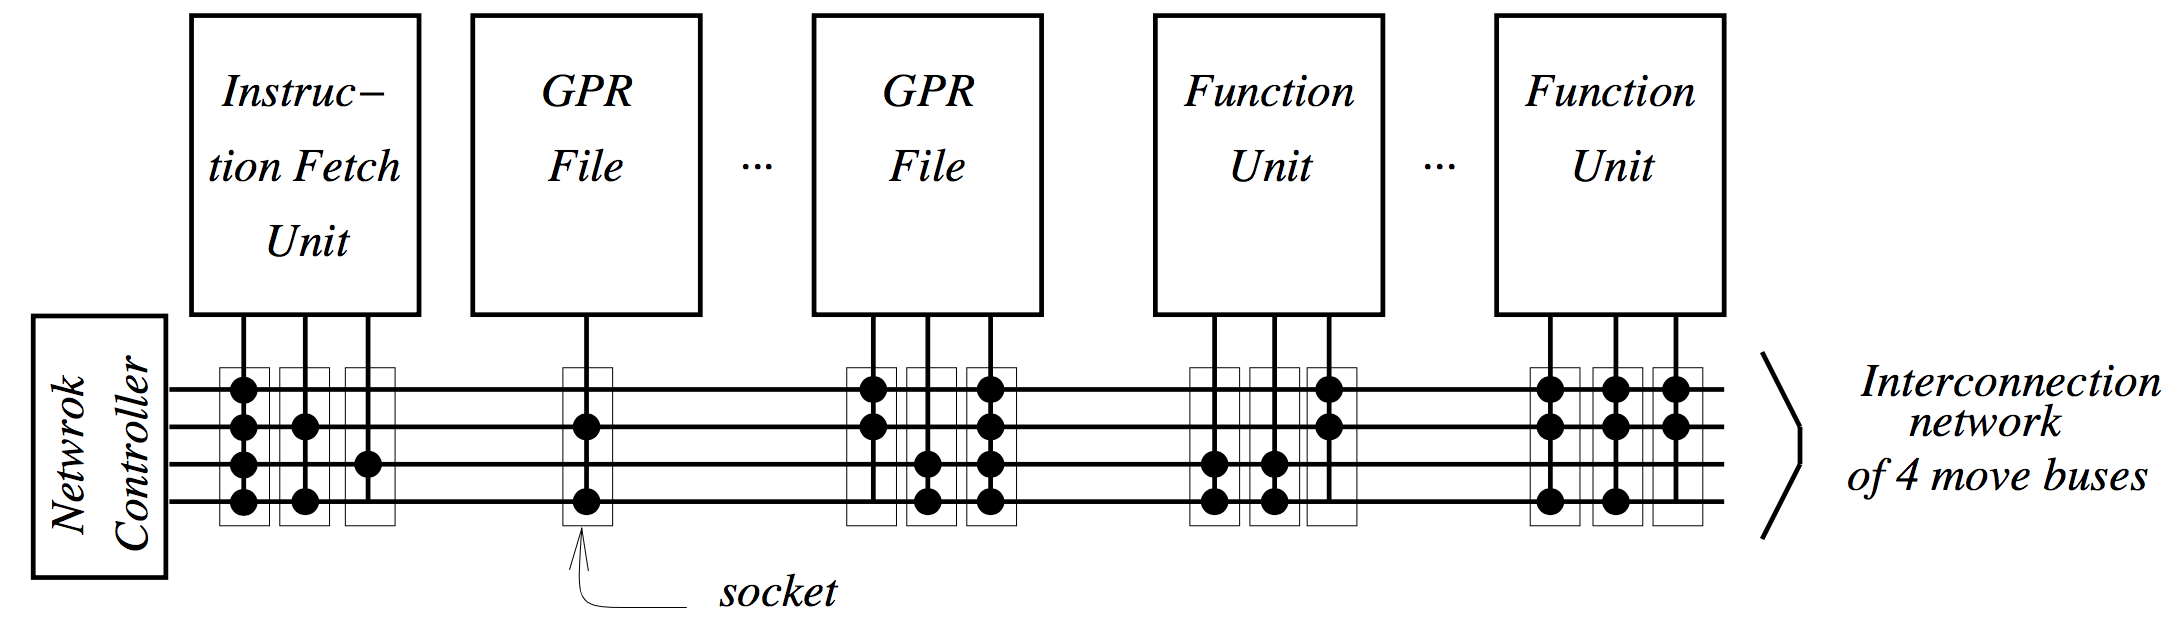
\includegraphics[width=.8\textwidth]{figures/tta_structure}
\caption{General structure of a TTA with interconnect network driven by data transports.}
\label{fig:tta}
\end{figure}

%\lstset{style=customasm}
\begin{lstlisting}
add r1, r2, r3  # define r1 with r1 = r2 + r3
sub r4, r2, 6   # define r4 with r4 = r2 - 6
sw  r4, r1, 0   # store result at address r1
\end{lstlisting}

First step is to translate each $n$-operand $m$-result operation into $n+m$ moves (so called $n$ \emph{operand moves} and $m$ \emph{result moves}). \texttt{O1} and \texttt{O2} are input ports of the FU and \texttt{R} indicates the output (result) of a FU.
%Insert more text explaining both fragments above and below this paragraph.

\begin{lstlisting}
r2 -> O1add ; r3 -> O2add ; Radd -> r1
r2 -> O1sub ; r6 -> O2sub ; Rsub -> r4
r1 -> O1sw  ; r4 -> O2sw
\end{lstlisting}

Let us assume that there are two FUs named \texttt{alu1} and \texttt{alu2} for ALU operations, and one FU named \texttt{ls} for load-store operations. The suffixes `\texttt{alu1}', `\texttt{alu2}', and `\texttt{ls}' indicate the FU on which the operation is executed.
If the above fragment would be scheduled such that the distance between the final operand and a corresponding result move should be at least the latency of the FU. Then the following (TTA assembly) code may be obtained:

\begin{lstlisting}
r2 -> O1add.alu1 ; r3 -> O2add.alu1 ; r2 -> O1sub.alu2 ; r6 -> O2sub.alu2
Radd.alu1 -> r1  ; Rsub.alu2 -> r4
r1 -> O1sw.ls    ; r4 -> O2sw.ls
\end{lstlisting}


\textbf{Bypassing:} The outputs of the add and subtract operations can be directly moved to the load-store unit. This reduces the schedule by one cycle, however, the number of moves does not change.

\begin{lstlisting}
r2 -> O1add.alu1; r3 -> O2add.alu1; r2 -> O1sub.alu2    ; r6 -> O2sub.alu2
Radd.alu1 -> r1 ; Rsub.alu2 -> r4 ; Radd.alu1 -> O1sw.ls; Rsub.alu2 -> O2sw.ls
\end{lstlisting}

\textbf{Dead result move elimination:} Next it may occur that the values in \texttt{r1} and \texttt{r2} are not live anymore because they are used only once. In that case corresponding moves can be skipped. This gives the following schedule:

\begin{lstlisting}
r2 -> O1add.alu1 ; r3 -> O2add.alu1 ; r2 -> O1sub.alu2 ; r6 -> O2sub.alu2 
Radd.alu1 -> O1st.ls ; Rsub.alu2 -> O2st.ls
\end{lstlisting}

The optimizations that is discussed here for TTA also apply on a wide SIMD architecture, which is discussed in Section \ref{sec:datapaths}. However, their approach can not be used because the SIMD architecture is an operation triggered architecture, data transports are a given. More information on explicit bypassing for TTAs can be found in the work of Hoogerbrugge et. al. \cite{tta, tta_codegen}.

%TODO read chapter 7 and cite to it, add words about TTA compiler. Then can be used yes/no

\begin{figure}[b!]
\centering
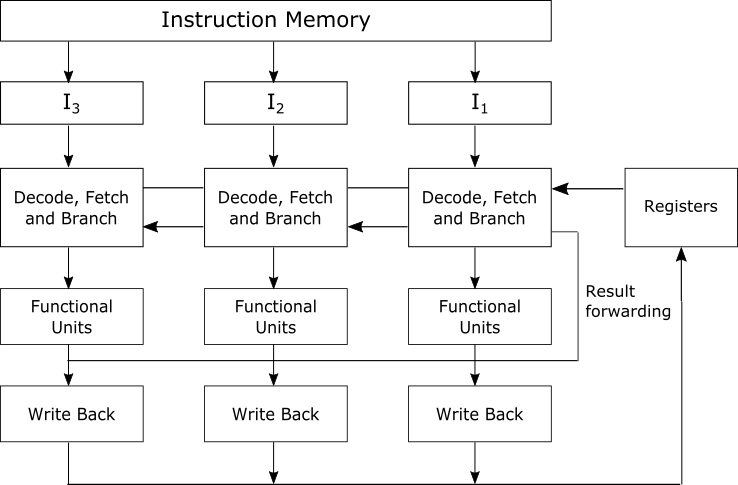
\includegraphics[width=.65\textwidth]{figures/vliw_forwarding}
\caption{Block diagram of VLIW architecture with bypassing.}
\label{fig:vliw}
\end{figure}

\subsubsection{Very Long Instruction Word Architectures}
The \emph{Very Long Instruction Word} (VLIW) architecture is designed to optimize \emph{Instruction Level Parallelism} (ILP) by executing multiple instructions in parallel.
Although RISC architectures take advantage of temporal parallelism by using hardware pipelining (explained in Chapter \ref{sec:datapaths}), VLIW architectures take advantage of spacial parallelism by using multiple functional units to execute several operations concurrently. 

Figure \ref{fig:vliw} shows a generic block diagram of a VLIW machine that has multiple instruction issues (three in this example), and each issue has its own decode stage and functional units. The figure also illustrates how the bypass network connects the outputs of the FUs back to the ID stage, allowing results to be forwarded. For VLIW architectures, the complexity of the bypass network grows linearly with the size of the instruction word. Furthermore, traditionally the register file requires $n$ write and $2n$ read ports, where $n$ is the length of the instruction word. This may require a more hungry register file as the power efficiency degrades when increasing the number of ports on the register file \cite{compiler_driven_power_opt}. However, this requirement can be relaxed by clustering, where each cluster may have a dedicated register file, which is often done in modern VLIW architectures.\\

A reconfigurable VLIW architecture is developed in the $\rho$-VEX project at the University of Technology in Delft \cite{p-vex}. This architecture also considers explicit bypassing and other configurable design options, e.g. configurable issue-width, functional units and bit-width of the data.

However, their implementation can not be used because (i) they are using a gcc based compiler instead of a LLVM based compiler and (ii) not a lot of implementation details have been given in their paper.



%\subsubsection{ReMove}
%Another architecture that exploits explicit datapath architectures is the ReMove architecture \cite{remove}. That work focusses on scheduling for partially connected architectures with explicit datapaths. The ReMove architecture is similar to a VLIW, having multiple FUs, however here they have an interconnect network that connects the FUs to the RF. The scheduling algorithm used in this work can not be used in our work, because similar to the legacy compiler for SIMD, this project has a custom backend, which can not be reused for LLVM. However, the basic principles of the scheduling algorithms proposed in this work are still valid and may be reused for our work.

%\section{Scheduling and Register Allocation}
%First of all, from the existing scheduling algorithms, Swing Modulo Scheduling (SMS) seems to be a suitable scheduling approach. It is a heuristic approach that is able to deal efficiently with software pipelining. Furthermore, it is known for its outstanding performance and low computational cost. The generated schedules are near optimal in terms of initiation interval and register requirements \cite{swingmodulo_paper, swingmodulo_thesis}. We consider this a candidate scheduler to use.

%Furthermore, the following literature discusses register allocation for SSA-based programs that solves coloring problem optimally in quadratic-time optimal by decoupling coloring, spilling and coalescing \cite{ra}. This technique may allow us to implement a custom register allocator that solves the problem in polynomial time.

%Finally, there is another project, called Unison. They solve scheduling and register allocation and other code generation tasks by translating them into combinatorial problems and solve them together with constraint programming \cite{unison}. We consider this a candidate constraint solver to use because it can be easily integrated with LLVM.

\subsection{Legacy compiler}\label{sec:legacy_comp}
S. Dongrui et al. proposed this processor architecture \cite{simd} while attaining his PhD \cite{dongrui}. The target wide SIMD architecture was design during that time and the compiler that was developed then has many issues. To start, the compiler has a LLVM frontend and a mostly in C++ implemented backend which is not according to LLVM standard. Therefore, it requires a frontend based on an old version of LLVM and since its front-end evolves over time, it is preferable to be able to update this to the newest version. \\

With C code applications as input language, the compiler can only compile to non-vectorized (CP only) instructions. To generate vectorized code an effort had been made to take OpenCL code as input language \cite{dongrio2}. However, only a subset of OpenCL is supported. Moreover, compilation does often generate incorrect code, or none at all. \\


In his work he shows that the register file is one of the most frequently used, and most power-hungry components in a processor. Therefore, he introduced an explicit datapath to further improve energy efficiency on this extremely energy efficient processor architecture. Moreover, efficient code generation for such architecture is key to achieve high energy efficiency for the whole processor. For this reason, the efficiency of the generated code is improved by standardizing the compiler to a frequently used framework. Namely, by standardizing to LLVM. This way we may benefit from developments in the field of compilers and from improvements made to the LLVM framework.
%A compiler had already been developed during the design phase of the target wide SIMD architecture \cite{dongrui}. That compiler has an assembler that can translate from assembly to object code and the compiler can translate C code to scalar only- and OpenCL to vectorized assembly code or object code. That compiler consists of a LLVM front-end and the back-end is developed in C++, but not within the LLVM framework.

%The legacy compiler was developed by the ES group in 2003. We will use the SIMD architecture as it was designed during that time . The legacy compiler has a custom backend for the SIMD architecture that can generate code for explicit datapaths \cite{dongrio1}, but it can only compile C code to non-vectorized instructions or a small subset of hand-touched OpenCL code that also requires manual insertion of custom pragmas to compile for vectorized code \cite{dongrio2}. Our goal is to overcome certain limitations and improve the compilers maintainability.
 

%Dongrio's simd work 

\subsection{Basic Compiler Design}\label{sec:basic_compiler_design}
This section explains an initial design of a SIMD back-end designed within LLVM developed by L. Zhenyuan \cite{liu_zhenyuan}. He started to build a back-end in LLVM for the same purpose, but with a different goal, namely how to generate efficient vectorized code within LLVM. In order to support vector instructions, LLVM's auto-vectorizer has been used and intermediate code optimization passes have been implemented to generate SIMD specific intrinsics, that are, in turn, transformed to vector instructions and shuffle operations. 

His work gives a basic design for this back-end that targets a wide SIMD architecture. The compiler that he developed is taken as a starting point, and is maintained, improved and extended which is discussed in later sections. When building a back-end in LLVM, first the instructions and registers have to be defined. Then illegal operations and types can be converted to legal ones. Then during instruction selection, LLVM knows how to match DAG nodes to known instructions. The supported instructions and registers for this architecture are defined first. To support some special features of this architecture, custom passes are added to this back-end, which will be described in detail, see Chapter \ref{sec:code_generation}, where our contributions to this work are discussed. Furthermore, an assembler and a linker have been implemented as separate projects, which will briefly be discussed here as well.

\subsubsection{Supported Instructions}
All the instructions which have been defined in this compiler are listed in this part, with the corresponding brief explanations. The details of ISA can be found in Appendix \ref{appendix:isa}.
\begin{itemize}
	\item \textbf{Arithmetic and Logic Instructions:} \texttt{add}, \texttt{addi}, \texttt{sub}, \texttt{muli}, \texttt{mulu}, \texttt{mului}, \texttt{or}, \texttt{ori}, \texttt{and}, \texttt{andi}, \texttt{xor}, \texttt{xori}, \texttt{sll}, \texttt{slli}, \texttt{sra}, \texttt{srai}, \texttt{srl} and \texttt{srli}.\\
The instruction with suffix "I" is used to handle immediate value operand, which is referred to as I-type instructions. The suffix "U" means it is used for unsigned values. For others, the two input operands are both registers, which are commonly referred to as R-type instructions.
	\item \textbf{Flag Set Instructions:} \texttt{sfeq}, \texttt{sfne}, \texttt{sfles}, \texttt{sflts}, \texttt{sfges}, \texttt{sfgts}, \texttt{sfleu}, \texttt{sfltu}, \texttt{sfgeu} and \texttt{sfgtu}.\\
The flag set instructions are used for comparison. If it is true, the flag register is set. The suffix "S" represents a signed value, while the suffix "U" represents an unsigned value.
	\item \textbf{Conditional Move:} \texttt{cmov}.\\ This is usually used with flag set instructions. If the flag is set, the value in the input operand is moved to the output operand.
	\item \textbf{Immediate Extension:} \texttt{simm} and \texttt{zimm}.\\ These two instructions are used to extend the immediate value from 8 bits to 26 bits. The maximum immediate value could be $2^{26}-1$, instead of $2^8-1$. The details of these two instructions will be discussed in Section \ref{sec:immediate_ext}. In addition, a larger immediate value requires a sequence of instructions to be executed.
	\item \textbf{Conditional Branch:} \texttt{bf} and \texttt{bnf}.\\ These two instructions also work with flag set instructions. By using the branch in- structions, the program can branch to the target address if the flag is set (with BF) or not set (with BNF).
	\item \textbf{Jump Instructions:} \texttt{j}, \texttt{jr}, \texttt{jal} and \texttt{jalr}.\\ The difference with the conditional branch instructions is that the jump does not need to check the flag register, which is normally used during function call and return.
\end{itemize}

\subsubsection{Register Configuration}
There are two main register classes. Although each PE has its own register file in our architecture, it is not necessary to define a specific register class for every PE register file. One reason is the size of the PE array is configurable and the number of the vector register classes cannot be dynamic. Another reason is, the vector array actually is a single issue slot, which executes the same instruction for all PEs. It is sufficient to define one register class for the entire PE array. Each vector register defined in the back-end represents a line of registers in the PE array.

\begin{table}[t]
\caption{Registers configuration.}
\begin{center}
\begin{tabular}{@{}l l l@{}}
\toprule
\textbf{Scalar Register} & \textbf{Vector Register} & \textbf{Purpose} \\ \hline
\texttt{r0} & \texttt{v0} & Constant value zero \\
N/A & \texttt{v1} & Constant PE index \\
\texttt{r3}$\sim$\texttt{r4}  & \texttt{v3}$\sim$\texttt{v4} & Return registers \\
\texttt{r5}$\sim$\emph{r8} & \texttt{v5}$\sim$\texttt{v8} & Argument passing registers \\
\texttt{r9} & N/A & Link register \\ 
\texttt{r10} & N/A & Frame pointer \\
\texttt{r11} & \texttt{v11} & Stack pointer \\
\texttt{r1}, \texttt{r2} and \texttt{r12}$\sim$\texttt{r31} & \texttt{v2}, \texttt{v9}$\sim$\texttt{v10} and \texttt{v12}$\sim$\texttt{v31} & General purpose registers \\
\bottomrule
\end{tabular}
\end{center}
\label{table:register_conf}
\end{table}%
%TODO: add text that goes by this, and optionally change lists in tables.

Table \ref{table:register_conf} shows the register configurations of both CP and PE-Array.
Both \texttt{r0} and \texttt{v0} are connected to ground and contain constant value zero. \texttt{v1} is a special register, which contains the index of local PE. Note that, there are two stack pointers, \texttt{r11} and \texttt{v11}. As mentioned before, considering there are two separated data memory, a double frame stack is needed for the CP and PE-Array to access their memories directly and reduce the expensive data communication. Therefore, two stack pointers are defined to point to the top of scalar and vector frame stacks respectively. The details of separate frame stacks is not described here, but can be found in L. Zhenyuans thesis \cite[Chapter~4]{liu_zhenyuan}.

\subsubsection{Vectorizer}
 Support for LLVM's Auto-Vectorizer has been developed by L. Zhenyuan. He added support for this to our back-end during his time \cite[Chapter~5]{liu_zhenyuan}. He defined a couple of patterns to match and IR level transformations that transform loops to vector instructions and shuffle operations. Furthermore, he added a cost function to decide whether to vectorize a given loop automatically. However, sometimes the auto-vectorizer fails to vectorize a simple loop. In those cases, pragmas are manually inserted directly before a loop in the C code. Clang uses these pragmas for making decisions on whether or not to vectorize a given loop. In the end, this may give better results, as will be shown in Chapter \ref{chapter:evaluation}.
 
 Supported vector types are:
 \texttt{v1i32}, \texttt{v2i32}, \texttt{v4i32}, \texttt{v8i32}, \texttt{v16i32}, \texttt{v32i32}, \texttt{v64i32}, \texttt{v128i32}, \texttt{v256i32}, \texttt{v512i32}, \texttt{v1024i32} and \texttt{v2048i32}.\\
	The actual legal vector type should be equal to or smaller than the \texttt{PENum}. \texttt{PENum} is a variable defined in the back-end, which can be configured using \texttt{pe-num} flag. The default value is 8, in which case the legal vector type can only be \texttt{v1i32}, \texttt{v2i32}, \texttt{v4i32} and \texttt{v8i32}.

\subsubsection{Linker and Assembler}
An assembler has been implemented that can parse assembly code and translate it into binary code. Furthermore, a linker has been developed which takes one or more binary files and combines them into a single executable file. These have been developed as separate projects and within the LLVM framework. Unfortunately, the linker still has some problems that need to be resolved before it can be used. %TODO go deeper into limitations of the lld linker
Therefore, a custom linker is chosen instead of the standard linker supplied by LLVM. We would benefit from using LLVM's linker because the custom linker can work only on a single file. Unfortunately, this linker can not be used yet because it is a work in progress.%work in progress

%TODO: add bypassing, auto and expl, (from slides)



%\clearemptydoublepage

% TODO: rewrite expl, or merge in other chaps
%\chapter{Explicit Bypassing}\label{chapter:explicit_bypassing}
%Suppose that we have a four stage pipeline where each instruction takes only one cycle. Let $a$ and $b$ be two instructions with a R/W dependency, i.e. instruction $b$ uses a value that is defined by instruction $a$. During the first cycle, instruction $a$ is fetched from Instruction Memory (IMEM). In the second cycle, instruction $a$ selects the operands from the RF, and instruction $b$ is fetched from IMEM. During the third cycle, instruction $a$ is in the execution stage, while instruction $b$ selects the operands that it needs. During the fourth cycle, instruction $a$ is in the WB stage, where it writes the result back to the RF, and instruction $b$ is in the execution stage.

Without bypassing, the result of instruction $a$ will be available only after it is written back. On the other hand, when we do have a bypass network, we may forward the result of an instruction to another instruction. In our example, we have forwarded the result of instruction $a$ directly to the operand of instruction $b$, as indicated by the vertical arrow that goes from the first to the second instruction in Figure \ref{fig:bypass_principle}. A result of an instruction may be accessed a cycle earlier when we compare with and without bypassing, however the target architecture has either explicit or implicit bypassing, which are both access a result a cycle early. So, in terms of cycles it makes no differences whether to use explicit or implicit bypassing. However, as you will see later, explicit bypassing has an advantage over implicit bypassing.

\begin{figure}[H]
\centering
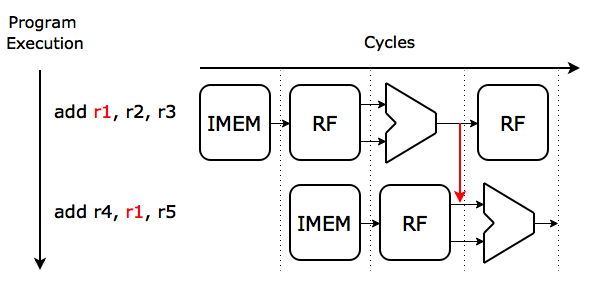
\includegraphics[width=.6\textwidth]{figures/bypassing_principle/05_bypassing_principle}
\caption{Illustration of bypassing and software pipelines in general.}
\label{fig:bypass_principle}
\end{figure}

With bypassing, we have wires that connect outputs of EX stage to the ID stage and we have this for each bypass source. 

\section{Implicit Bypassing}
With implicit bypassing we have wires that connect the outputs from EX stage to the ID stage, as illustrated in Figure \ref{fig:impl_bypass_principle}. Furthermore, we also have wires that go from the WB stage to the ID stage, however this is not shown in this example. To detect bypasses, the HW matches whether the operands of the currently issued instruction to the destination address of previously issued instructions. If we have a match, and the result is still available in the pipeline, we can then bypass it. We have a mux that controls which inputs are used, i.e. a value from a register, or a value from a bypass. The bypass detection hardware is in control which of these values is selected.

\begin{figure}[t]
\centering
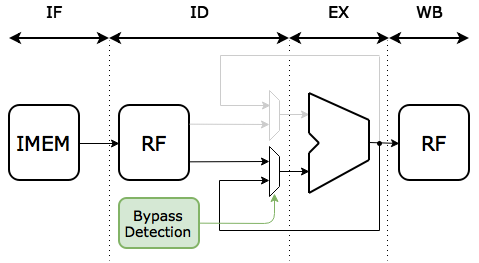
\includegraphics[width=.5\textwidth]{figures/impl_bypassing_principle/03_implicit_bypassing_principle}
\caption{Illustration that shows the basic principles of implicit bypassing.}
\label{fig:impl_bypass_principle}
\end{figure}

\section{Explicit Bypassing}
For explicit bypassing, we have similar wires that connect outputs of EX stage to the ID stage as we have in implicit bypassing. However, with explicit bypassing the compiler is responsible for detecting when we can bypass the result of a instruction. In Figure \ref{fig:exp_bypass_principle_r} we show that the control signal to the mux, that selects the input from a register or from a bypass, is now controlled by the compiler. The compiler encodes this information in an instruction. This way, during instruction decoding, the control signal is immediately available. Furthermore, we have a read-enable flag on the register file. If we then want to take the data from a bypass, we can set this value to zero. This way, we can avoid speculative reads accesses from the RF. We use the same signal from the ID stage, to control the read-enable on the register file and the signal that controls the mux. 

\begin{figure}[H]
\centering
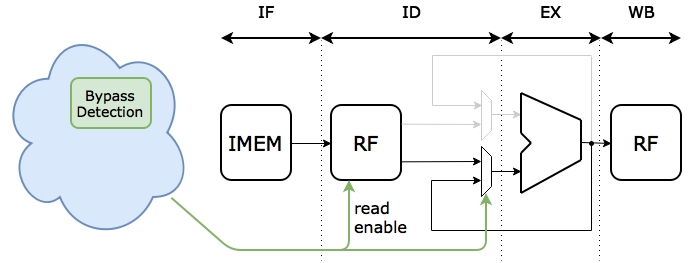
\includegraphics[width=.7\textwidth]{figures/expl_bypassing_principle/01_explicit_bypassing_principle}
\caption{Illustration that shows the basic principles of explicit bypassing, read enabled port on RFs to avoid unnecessary reads.}
\label{fig:exp_bypass_principle_r}
\end{figure}

We can use the liveliness information during compilation to determine whether a variable is live after it is used. If the variable is not live after it is used often indicated by a kill of a variable, we can disable the write on the register, since it will not be needed anymore. Figure \ref{fig:exp_bypass_principle_rw} illustrates this by adding a write-enable flag on top of the read-enable that was already present from Figure \ref{fig:exp_bypass_principle_r}. Adding a write-enable flag allows us to avoid speculative write accesses to the RF.

\begin{figure}[t]
\centering
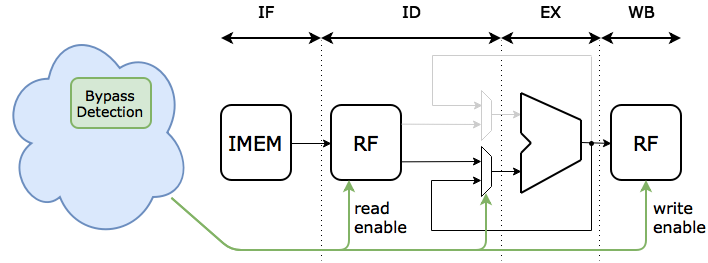
\includegraphics[width=.7\textwidth]{figures/expl_bypassing_principle/02_explicit_bypassing_principle}
\caption{Illustration that shows the basic principles of explicit bypassing, read enabled port on RFs to avoid unnecessary reads and write enable port to avoid speculative writes.}
\label{fig:exp_bypass_principle_rw}
\end{figure}

A significant difference between explicit and implicit bypassing is that some writes accesses to the register file may be avoided for explicit bypassing, while this is can not be done with implicit bypassing.

In general, the result of an instruction will remain in the pipeline  scheduled in the future, in order to see whether the result of an operation will be used later on, which is not possible at runtime.

%%%%%%%%%%
%\section{Bypass Sources}

The target architecture has operand isolation, which we mentioned in Chapter \ref{sec:processor}. Because of this, the output of the function units do not toggle, i.e. are only calculated when the operand registers change. This has as a side effect that when a function unit is not used, the output register remains the same. This means that a instruction can be bypassed, as long as we do not use the function unit on which it was executed. We have given the bypass sources for our architecture below, in Table \ref{table:bypass_alias}. Here we have provided all bypass sources for the four stage and five stage pipeline

\begin{table}[H]
\caption{Alias for each bypassing source, $BP\_src$ in Figure \ref{fig:4_stage} and Figure \ref{fig:5_stage}.}
\begin{center}
\begin{tabular}{@{}llll@{}}
\toprule
\multirow{2}{*}{\textbf{Register:}} & \multirow{2}{*}{\textbf{Bypass source:}} & \multicolumn{2}{c}{\textbf{Alias}:} \\ \cline{3-4}
 & & \textbf{4 stages} & \textbf{5 stages} \\
\hline
\emph{r27} & $BP\_src27$ & N/A & ALU1 \\ 
\emph{r28} & $BP\_src28$ & LSU & LSU \\
\emph{r29} & $BP\_src29$ & MUL & MUL \\ 
\emph{r30} & $BP\_src30$ & ALU & ALU2 \\
\emph{r31} & $BP\_src31$ & WB & WB \\
\bottomrule
\end{tabular}
\end{center}
\label{table:bypass_alias}
\end{table}%

%%%%%%%%%%%%

We will now show with an example that avoiding speculative write accesses may reduce Register Pressure (RP).

%TODO: move this to a better place, or explain this in one of the previous sections
%this being that we have multiple bypassing sources, we specify them as if they were a register, and the following registers map to the following bypassing sources.
%One from each FU, one from WB and an additional one from blala
%With automatic bypass we actually always bypass from WB, because otherwise each instruction would take one more cycle. Namely one or two execution stages and a wb stage after which the result is the register.
%With explicit bypassing the compiler can avoid some accesses to RFs by explicitly specifying the datapath.

%Connect to TTA architectures, use findings of Johan Janssen.

%Show the need for this like done in Johans' paper. (and in lucs paper)

%Different approches
% - Naive implementation
% - Scheduling pass to automate it
% - Combine RA and scheduling to do it better.
% - Use LLVMs way to describe explicit bypassing, namely targetItinirary.td

\begin{lstlisting}[caption=Example code fragment where no bypassing is specified., label=lst:nobypass]
mul <@\textcolor{red}{r1}@>, r2, r3
add r4, <@\textcolor{red}{r1}@>, r5
\end{lstlisting}

Listing \ref{lst:nobypass} shows a code fragment with a multiplication and an addition. We have a flow dependent dependency. Namely, the result of the multiplication is used by the addition.

\begin{lstlisting}[caption=Example code fragment avoiding a read access., label=lst:operandbypass]
mul <@\textcolor{red}{r1}@>, r2, r3
add r4, <@\textcolor{red}{MUL}@>, r5
\end{lstlisting}

In Listing \ref{lst:operandbypass} we have replaced the use of $r1$ with $MUL$. This indicates that we do not take the first operand from the RF, but from a bypass instead. Since we obtain the result of the multiplication from the bypass network, we do not require a read access to $r1$ anymore.
%This is also done for the implicit bypassing approach, however since we have more bypass sources for the explicit bypassing variant, we expect that operand bypassing is done more aggressively.

\begin{lstlisting}[caption=Example code fragment avoiding a read and a write access., label=lst:fullbypass]
mul <@\textcolor{red}{--}@>, r2, r3
add r4, <@\textcolor{red}{MUL}@>, r5
\end{lstlisting}

When the result of $r1$ is not needed anymore, for example, the live range of $r1$ spans no further than this addition, the write access can be avoided. By specifying $--$ as destination, the result will not be written back, as illustrated in Listing \ref{lst:fullbypass}. Register $r1$ is now completely removed from the example, effectively freeing that register. We have now reduced RP by one, since we require one less register. The freed register can be used for other calculations, which may lead to a higher performance.

%%%%%%%%%%%%%%%%%%%%%%%%%%%%


%HERE WE SHOW ALL DIFFICULT CASES, i.e. First instruction of loop body is bypassed from last instruction of loop body.
\section{Joint Point Issue}
In the following example we will illustrate a special case that may be taken into consideration.

\begin{lstlisting}[caption=Example code fragment where bypassing over backedge of a loop iteration is not possible., label=lst:bypassloop1]
      lw <@\textcolor{red}{r6}@>, r10, 5
loop: 
        <@\raisebox{-1pt}[0pt][0pt]{$\vdots$}@>
      
      sfeq <@\textcolor{red}{r6}@>, r0
      bnf loop
      addi <@\textcolor{red}{r6}@>, <@\textcolor{red}{r6}@>, -1

        <@\raisebox{-1pt}[0pt][0pt]{$\vdots$}@>
\end{lstlisting}

When we access the loop counter for the first time in Listing \ref{lst:bypassloop1}, $r6$ can be bypassed from the $LSU$. However, in consecutive iterations, we would bypass it from the $ALU$ instead. Listing \ref{lst:bypassloop2} shows that adding an instruction before entering the loop allows us to bypass the value in consideration. We may profit from this if a lot of loop iterations are processed.

\begin{lstlisting}[caption=Example code fragment where bypassing over the backedge of a loop iteration is possible., label=lst:bypassloop2]
      lw <@\textcolor{red}{--}@>, r10, 5
      add <@\textcolor{red}{r6}@>, <@\textcolor{red}{LSU}@>, 0
loop: 
        <@\raisebox{-1pt}[0pt][0pt]{$\vdots$}@>
      
      sfeq <@\textcolor{red}{ALU}@>, r0
      bnf loop
      addi <@\textcolor{red}{--}@>, <@\textcolor{red}{r6}@>, -1

        <@\raisebox{-1pt}[0pt][0pt]{$\vdots$}@>
\end{lstlisting}

%TODO: leg dit eens fatsoenlijk uit joh
Here we want to apply bypassing to bypass the result of the last add instruction in the loop before we branch to the first instruction in the loop. However, when we go in the loop for the first time, $r6$ comes from the LSU instead of the ALU. Therefore, sometimes it is necessary to insert an instruction before we enter a loop to bypass over loop iterations.

%\section{Proposed Approaches}
%We will investigate in different approaches to implement software bypassing on top of the SIMD architecture within LLVM. Each of these approaches will be evaluated. The kernels that we will use as means of evaluation are discussed in Chapter \ref{sec:benchmark}.

%\begin{enumerate}
%\item Naive approach in which we will add a pass on top of the existing scheduler to apply software bypassing whenever possible. In this approach, explicit datapaths are created after scheduling and register allocation.
%\item Use LLVMs framework to express the processors pipeline stages and bypassing sources. This way LLVM will apply software bypassing. This will be a good reference for our final approach.
%\item Implement a bypass aware combined scheduling and register allocation algorithm. We need to investigate what steps need to be taken to implement a custom scheduler in LLVM.
%TODO: introduce the need for combined scheduling and RA..... 
%\end{enumerate}
%Incorporate notes from 21/22 februar, write a long text to discuss all of them. This way we have motivation for each of the proposed solutions.

%TODO: make example for each approach.

%\section{Method of Evaluation}\label{sec:benchmark}
%Discuss the kernels that we will use to evaluate the different approaches. We will use RTL synthesis to emulate the processors behaviour on certain kernels and model the energy consumption for each of the approaches, for the transparent bypassing variant, and finally for a by hand optimized and bypassed variant. This should give us an "optimal" energy reduction compared to the energy reduction that we achieved, with transparent bypassing as reference.




\chapter{LLVM-based Compiler for SIMD}\label{chapter:compiler}


%\section{Design Method}\label{sec:design_method}
This chapter focusses on each of the code generation phases and what our contributions are to this compiler. This chapter describes how a compiler without support for explicit datapaths (which is described in Section \ref{sec:basic_compiler_design}) is maintained and extended to a compiler with support for explicit datapaths. 

%Discuss maintaining, process of porting from llvm3.8 to LLVM4.0, and discuss new version LLVM5.0. Mention that this upgrade to 4.0 also drastically improved vectorization because the community develops this constantly. (maybe add example of CNN)

%TODO: move vectorization to here? Noooo.

\section{Back-end Code Generation}\label{sec:code_generation}
This section briefly discusses each of the code generation stages, which includes custom passes and standard passes supplied by the LLVM framework. Before generating code, it uses LLVM's front-end to translate a high-level language to an intermediate representation, called LLVM-IR which can be further optimized and used as input for our back-end. The code generation passes in the back-end specific compiler can be categorized in three major categories.
%include an image with the pipeline having all these components.

%TODO: refere to problem where instr have no common operand, so it seems unrelated. 

%TODO: add text that explains the color, instruction selection is copied mostly from another architectures, and was already updated according to our architecture. / Hazard recognizer has partially been copied from other architectures, but was not suitable and has, therefore, been modified and tested. / Delay slot is a custom pass that was already implemented, but we have modified it to be more efficient. / Packetizer pass is as delivered, with a minor modification with hardly any efford.  / Bypass Regs is a custom pass that we developed during the duration of our work.

Firstly, the top row in Figure \ref{fig:simd_backend} shows passes that work on creating a schedule. The second row illustrates a sequence of compilation passes that do back-end specific transformations. Here special features that our architecture has are taken care of. At last, with an LLVM internal representation of back-end specific code for the target architecture, it emits assembly or ELF object code (depicted in the rightmost part of the image) that the processor can understand.

\begin{figure}[H]
\centering
\hspace*{-.12in}
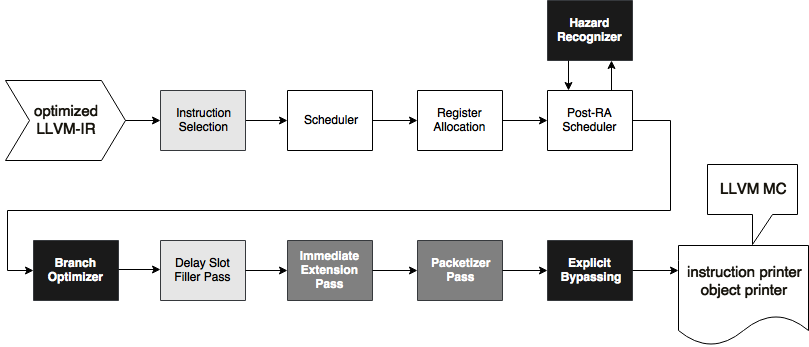
\includegraphics[width=\textwidth]{figures/code_generation}
%TODO: change orange to yellow and yellow to orange in picture. 
\caption{Overview of the phases that the back-end is comprised of.}
\label{fig:simd_backend}
\end{figure}

Note that the passes are marked from light to dark, where a black background means that the pass was created during this project and are the main contributions of this work. Dark grey indicates that a pass is extended or improved, light grey indicates the pass has hardly changed and a white background means that the pass is supplied by LLVM.

%A list of all components that follow in the following section.
\begin{itemize}
	\item \textbf{Instruction Selection:} Uses a DAG, called \texttt{SelectionDAGs}, an abstraction for code representation suitable for phases ranging from instruction selection, legalization to lowering. Instruction selection is implemented in  \texttt{SimdISelDAGToDAG}, which is derived from \texttt{SelectionDAGISel} and consists of a bunch of transformations to transform specific instructions into instruction that are supported by our architecture. For example, transforming operations on immediate values with a value higher than one byte is partially implemented here. Lowering nodes of a DAG is done in \texttt{SimdISelLowering}, which is derived from \texttt{TargetLowering}. There the SIMD intrinsics and ISD instructions are lowered to \emph{Machine Instructions} (MI) and sequences of MIs.
%\item \textbf{Scheduling:} Transforms a directed acyclic graph into an ordered list of instructions.
%\item \textbf{Register allocation:} Assigns physical registers to virtual registers of a list of instructions in SSA form.
	\item \textbf{Instruction Scheduler:} MIScheduler supplied by LLVM\\
MIScheduler is an instruction scheduler which supports VLIW scheduling. Considering there are two issue slots in this architecture, a VLIW scheduler would meet our requirements very well. One and two schedulers are defined for four-stage pipeline and five-stage pipeline respectively. The four-stage pipeline scheduler is the default one while the five-stage pipeline has the default one, and an additional post-register allocation scheduler.
	\item \textbf{Register Allocation:} Greedy Allocator supplied by LLVM\\
	The Greedy allocator is a default allocator in LLVM. Since there is no specific requirement to register allocation, for now, the default allocator is suitable. Apart from the default register allocator, there are more register allocators to choose from and, it is possible to implement a custom register allocator.
	\item \textbf{Post-Register Allocation Scheduler:} A second scheduling pass which is only needed when generating code for a five-stage pipeline configuration, and is disabled otherwise. The post-RA scheduler uses a hazard recognizer which decides whether to prefer certain instruction over other instructions to detect and resolve RaW hazards.
	\item \textbf{Hazard Recognizer:} Consecutive instructions may have hazards with the five-stage pipeline configured. That is when an instruction uses an operand defined in the previous cycle but has a latency of two cycles. For this thesis, we have implemented LLVM's \texttt{ScoreboardHazardRecognizer} to detect and resolve these hazards.
	\item \textbf{Branch Optimizer:} An inefficiency in the generated code was observed where two jump operations control the work flow, but one jump is not necessary when it jumps to the successor that follows immediately. 
	%TODO: check implements / extends / derived
	\item \textbf{Delay Slot Filler:} For this architecture, jump and branch instructions modify the program counter (PC) during the instruction decode stage. At that point, the instruction that follows the jump has already been fetched. The slot that follows a jump or branch instruction is called a delay slot. This pass aims to utilize delay slots by filling them with useful instructions.% that come after a jump or conditional branch instruction, i.e. instructions that modify the program counter.%VERIFY: `or e.g.?
	\item \textbf{Immediate Extension:} In principle, immediate operations have a one-byte immediate operand. However, sometimes you may want to use a larger immediate. This pass allows us to use a larger immediate operand using \texttt{zimm} and \texttt{simm} instruction. These instructions have an 18-bit operand that allows for larger constants to be used.% will be a prefix of the original 8 bits  or using a shift to put a value in a register (up to 32 bits).
	\item \textbf{Packetizer:} This pass creates VLIW bundles that consist of a scalar and a vector instruction, by consulting whether an issue slot is available on which the operation can execute. This pass implements VLIW packetizer supplied by the LLVM framework.
	\item \textbf{Explicit Bypassing:} This pass exploits explicit datapaths in the generated code by using the bypass network. This is developed as a post-processing pass, but can be replaced by any of the approaches discussed in Chapter \ref{sec:expl_bp_impl}.
	\item \textbf{Instruction Printer:} MC is a sub-project of LLVM, which uses \texttt{MCInst} to represent an instruction which is different from the code generators notion of a \texttt{MachineInstr}. MC is used during the last code generation stage when printing the instructions to a given output format. Printing for different output formats is further divided in binary format and SIMD assembly language in XAS-format. 
\end{itemize}

\begin{table}[t!]
\caption{Relations between architecture design features and code generation phases.}
\begin{center}
\begin{tabular}{@{}l l l@{}}
\toprule
\textbf{Feature} & \textbf{Code Gen. Pass} & \textbf{Explanation}\\ \hline
Hardware Pipeline 	& Delay Slot Filler 		& This pass utilizes the delay slots (which is\\
				&					& a product lockstep pipelining).\\
			 	& Hazard Recognizer 	& This pass is necessary for a five-stage \\
				&					& pipeline configuration where not all\\
				&					& instructions have a single cycle latency.\\
Bit-width 			& Immediate Extension 	& Lowering immediate operands is done\\
				&				    	& differently for different data bit-width. \\
ISA extension		& Instruction Selection 	& New instructions need to be described in\\
				& \& Instruction Lowering	& the back-end. \\
Explicit datapaths 	& Explicit Bypassing		& This optional pass is developed to exploit\\
				&					& explicit datapaths. It can be enabled\\
				&					& using compiler flag \texttt{-explicit}. \\
\bottomrule
\end{tabular}
\end{center}
\label{table:rel_feature_pass}
\end{table}%

The following sections give a more elaborate discussion on each custom pass and describe their relation to each other. However, before that have a look at Table \ref{table:rel_feature_pass} which gives an overview of the passes responsible for each of the features from Chapter \ref{sec:problem_statement}. 

%TODO: validate and update
\section{Custom Passes}
This section describes the custom passes in more detail. Dependencies and relations to other passes are described. Furthermore, it will discuss the entire toolchain, which includes an assembler, a linker, and a simulator. 

\subsection{Hazard Recognizer}\label{sec:hazard_recogn}
When generating code for a four-stage pipeline configuration, all instructions have a latency of one cycle. In that case, hazard recognition is not necessary.
In order to support code generation for a five-stage pipeline, a hazard recognizer has been developed. The hazard recognizer is used by the post-RA scheduler to determine whether two consecutive instructions can be scheduled after each other. 

\lstset{style=customasm}
\begin{lstlisting}
addi r13, r0, 14
addi r12, r0, 10
mul  r2,  r5, r13  # latency=2
mul  <@\hspace{1px}\textcolor{red!70!black}{r3}\hspace{1px}@>,  r6, r12  # latency=2
add  r2,  r2, <@\hspace{1px}\textcolor{red!70!black}{r3}\hspace{1px}@>   # RaW dependency
\end{lstlisting}

It detects hazards by considering whether an operation has a RaW dependency with instruction that came prior to it. A true hazard is when the instruction that came prior to it has a RaW dependency and a latency of more than one cycle. The \emph{post-register allocation} (Post-RA) scheduler does a linear scan through the list of operation and queries the hazard recognizer whether an instruction can be scheduled. When it detects a hazard, it will consider other instructions that are ready to be scheduled, and if there are none available without a hazard, it will insert a no-op and the processor will be stalled for a cycle.

%It recognizes hazards by looking at whether the current instruction to be scheduled uses a register that is defined by the instruction issued in the previous cycle, which also has a latency of more than one cycle. If this is the case, we have a hazard and the instruction under consideration can not be scheduled in the current cycle. At this point we will consider other instructions that are ready to be scheduled and if there are none available without hazards, we will insert a no-op.

\subsection{Branch Optimizer}
%WORKING RIGHT HERE. ADD EXAMPLE CASES FROM BRANCH OPT.
There were many double branch instructions in loop structures. Preliminary benchmarks already showed that a double branch instruction does not always help. For example, consider the assembly code fragments in Listing \ref{lst:br_opt_1} and Listing \ref{lst:br_opt_2}. Note that at this point, the delay slots that always follow after a jump or branch instruction are still absent because the delay slot filler pass has not run yet.

\captionof{lstlisting}{Fragment of assembly code to illustrate the first and second cases that are considered by the branch optimization pass.}\label{lst:br_opt_1}
\begin{center}
\hspace{2px}\begin{minipage}{.475\textwidth}
\begin{lstlisting}[frame=tlrb]
$BB1:
    addi   r1, r1, 1
    sfltsi r1, 64
    <@\hspace{1px}\textcolor{red!70!black}{bf}\hspace{1px}@>     <@\hspace{1px}\textcolor{red!70!black}{\$BB1}\hspace{1px}@>
    <@\hspace{1px}\textcolor{red!70!black}{j}\hspace{1px}@>      <@\hspace{1px}\textcolor{red!70!black}{\$BB2}\hspace{1px}@>
$BB2:      <@ $\hdots$@>
\end{lstlisting}
\end{minipage}\hfill
\begin{minipage}{.475\textwidth}
\begin{lstlisting}[frame=tlrb]
$BB1:
    addi   r1, r1, 1
    sfltsi r1, 64
    <@\hspace{1px}\textcolor{red!70!black}{bf}\hspace{1px}@>     <@\hspace{1px}\textcolor{red!70!black}{\$BB1}\hspace{1px}@>
$BB2:      <@ $\hdots$@>
           <@ $\hdots$@>
\end{lstlisting}
%\vspace{1.9em}
\end{minipage}
\end{center}

\begin{enumerate}
  \item The first case is where a block ends with a jump instruction to the block that immediately follows. The example shows a loop in which a counter is incremented until it reaches sixty-four. As long as the counter is less than that, the flag will be true and the branch is executed. When the counter increases, at some point the condition breaks and the flag becomes false. The program counter then points to the first instruction after the branch instruction, which is a jump instruction. However, the jump goes to the successor that immediately follows. When the jump is removed, the first instruction after the branch instruction is still the successor block that immediately follows. Hence the behaviour without that jump is identical and the superfluous jump can be removed.
  \item The second case has a branch instruction to the block that immediately follows and a jump to somewhere else. The first step then is to reverse the branch condition. This can be achieved by changing a \texttt{bf} (branch flag) instruction into a \texttt{bnf} (branch not flag) and vice versa. After the branch is reversed, the situation becomes a jump instruction to the block that immediately follows and a branch instruction to somewhere else. 
\end{enumerate}

\captionof{lstlisting}{Fragment of assembly code to illustrate the third case that is covered by the branch optimization pass.}\label{lst:br_opt_2}
\begin{center}
\hspace{2px}\begin{minipage}{.475\textwidth}
\begin{lstlisting}[frame=tlrb]
$BB2: <@$\hdots$@>
    sf condition  # set-flag
    <@\hspace{1px}\textcolor{red!70!black}{bf}\hspace{1px}@> <@\hspace{1px}\textcolor{red!70!black}{\$BB3}\hspace{1px}@>
    <@\hspace{1px}\textcolor{red!70!black}{j}\hspace{1px}@>  <@\hspace{1px}\textcolor{red!70!black}{\$BB2}\hspace{1px}@>
$BB3: <@$\hdots$@>
\end{lstlisting}
\end{minipage}\hfill
\begin{minipage}{.475\textwidth}
\begin{lstlisting}[frame=tlrb]
$BB2: <@$\hdots$@>
    sf  condition  # set-flag
    <@\hspace{1px}\textcolor{red!70!black}{bnf}\hspace{1px}@> <@\hspace{1px}\textcolor{red!70!black}{\$BB2}\hspace{1px}@>
$BB3: <@$\hdots$@>
     <@ $\hdots$@>
\end{lstlisting}
%\vspace{1.9em}
\end{minipage}
\end{center}

When a (double) jump intruction(s) jumps to a successor that immediately follows, the branch optimizer can always remove one jump with these cases.



%END BRANCH OPT DESCRIPTION

\subsection{Delay Slot Filler}
During the execution of a conditional branch or jump instruction the \emph{program counter} (PC) is modified while the instruction is in the \emph{instruction decode} (ID) stage. A side product of lockstep pipelining which is introduced in Chapter \ref{sec:datapaths}, is that when a jump instruction is being decoded in the ID stage, the next instruction with $PC = PC+4$ has already been fetched from IMEM before the jump is executed. Therefore, the instruction that is followed by the jump instruction is executed presumptuously, which is referred to as a delay slot.

%This slot will be executed before the instruction that the PC points at after modifying the PC and is called delay slot. %TODO: this paragraph can be shorter 

In order assure correct behaviour this pass intentionally 
%or initially (stood there in the first place)
places a no-op after each jump or branch instruction. However, sometimes it can do better. Namely, it can use an instruction from before the jump instead of a no-op. This pass performs a backwards search to look at the two instructions before the jump, and the instruction that comes after the jump, which are referred to as $prev_1$, $prev_2$, and $next$ respectively. When the backwards search does not fill the delay slot it intentionally insert a no-op, and if there is a vector operation that comes after the delay slot, it also inserts a vector-nop, so that the packetizer does not bundle it with the delay slot later on.

%\captionof{lstlisting}{Fragment of assembly code to illustrate behaviour of the delay slot filler.}\label{lst:delayslot1}
%\begin{center}
%\hspace{2px}\begin{minipage}{.475\textwidth}
%\begin{lstlisting}[frame=tlrb]
%BB0_1:
%    sfne r1, 7
%    add r3, r3, r1
%    bf BB0_1
%    nop
%\end{lstlisting}
%\end{minipage}\hfill
%\begin{minipage}{.475\textwidth}
%\begin{lstlisting}[frame=tlrb]
%BB0_1:
%    sfne r1, 7
%    bf BB0_1
%    add r3, r3, r1
%   <@ @>
%\end{lstlisting}
%%\vspace{1.9em}
%\end{minipage}
%\end{center}

%Possibly scrap this case distinction 
%Add picture from scratch paper showing these cases

\captionof{lstlisting}{Fragment of assembly code to illustrate behaviour of the delay slot filler for case one.}\label{lst:delayslot1}
\begin{center}
\hspace{2px}\begin{minipage}{.475\textwidth}
\begin{lstlisting}[frame=tlrb]
$BB1:
    v.add r3, r6, r14
    v.add r4, r5, r12
    j $BB1
    nop
\end{lstlisting}
\end{minipage}\hfill
\begin{minipage}{.475\textwidth}
\begin{lstlisting}[frame=tlrb]
$BB1:
    v.add r3, r6, r14
    j $BB1
    nop
    v.add r4, r5, r12
\end{lstlisting}
%\vspace{1.9em}
\end{minipage}
\end{center}

\begin{enumerate}
\item The first case is when the previous two instructions are both vector instructions. In that case, the vector instruction prior to the jump instruction can be moved to after it. Now the vector instruction that remains before the jump ($prev_1$) gets bundled with the jump instruction. If there was originally a scalar instruction after the jump instruction, it could get bundled with the vector instruction that is moved by this pass, later on by the packetizer. Therefore, it inserts a no-op to ensure the delay slot. %the instruction that came after is a scalar instruction, it would be merged with the filled instruction, therefore, in that case we need to add a nop, such that it bundles with the filled vector instruction.
\item When the instruction before the jump ($prev_1$) is a scalar instruction with no dependencies to the jump itself, it can moved to the delay slot. If a bundled instruction was moved, then it is done. Otherwise, if there are two vector operations prior to the jump instruction, it can move one of them to after the jump, thereby, fully utilizing the delay slot.

%\item[3] We also consider the case where $prev_1$ is a vector instruction, and $prev_2$ is not a relational or jump instruction. Since the first case considers both $prev_1$ and $prev_2$ vector instructions, we consider cases where $prev_1$ is a vector and $prev_2$ is scalar operation by this case. %todo: little more in depth explanation of this pass
\end{enumerate}

\captionof{lstlisting}{Fragment of assembly code to illustrate behaviour of the delay slot filler for case two.}\label{lst:delayslot2}
\begin{center}
\hspace{2px}\begin{minipage}{.475\textwidth}
\begin{lstlisting}[frame=tlrb]
$BB1:
    v.add r3, r6, r14
    v.add r4, r5, r12
    add   r3, r3, r1
    j $BB1
    nop
\end{lstlisting}
\end{minipage}\hfill
\begin{minipage}{.475\textwidth}
\begin{lstlisting}[frame=tlrb]
$BB0_1:
    v.add r3, r6, r14
    j $BB1
    add   r3, r3, r1
    v.add r4, r5, r12
   <@ @>
\end{lstlisting}
%\vspace{1.9em}
\end{minipage}
\end{center}

%\captionof{lstlisting}{Fragment of assembly code to illustrate behaviour of the delay slot filler for the third case.}\label{lst:delayslot3}
%\begin{center}
%\hspace{2px}\begin{minipage}{.475\textwidth}
%\begin{lstlisting}[frame=tlrb]
%BB0_1:
%    add r3, r3, r1
%    v.add r4, r5, r12
%    j BB0_1
%    nop
%\end{lstlisting}
%\end{minipage}\hfill
%\begin{minipage}{.475\textwidth}
%\begin{lstlisting}[frame=tlrb]
%BB0_1:
%    j BB0_1
%    add r3, r3, r1
%    v.add r4, r5, r12
%   <@ @>
%\end{lstlisting}
%\vspace{1.9em}
%\end{minipage}
%\end{center}
%todo: give case(s) that is not covered, followed by this line
The two cases covered by this pass are illustrated in Listing \ref{lst:delayslot1} and \ref{lst:delayslot2}. However, many delay slots are still not being utilized. Extending this pass such that more delay slots may be utilized will be added to future work.

%TODO: make case distinction here.
%\begin{enumerate}
%	 \item When the two operation before the jump instruction are both vector instructions,  
%\end{enumerate}
%TODO: make pseudo code of 

%Immediate extension 
\subsection{Immediate Extention}\label{sec:immediate_ext}
Most operations in Appendix \ref{appendix:i_type_instrs} have as last operand, a one byte immediate. However, sometimes one may need larger numbers. Therefore, constants are lowered during instruction selection. The following three cases are given:
\begin{enumerate}
\item When the immediate can be expressed with one byte it is trivial. It does not need to change anything.
\item When the immediate value is larger than one byte, but can be expressed with 26 bits, it adds a \texttt{zimm} or \texttt{simm} operation in front of it. These operations have a 18 bit immediate that represent the upper 18 bits for the operation that follows.

\begin{lstlisting}
simm 3          # 3 << 8 = 768
addi r3, r5, 12 # r3 = r5 + 768 + 12
\end{lstlisting}
\item If the immediate requires more than 26 bits, it requires a couple of instructions to be added in order to put the immediate value in a register. Firstly, the upper 6 bits go to a register and are shifted all the way to the left. Subsequently, the lower 26 bits are added to it using the previous cases.
%TODO: illustrate how the lowering is done.
\begin{lstlisting}
add  r3, r0, 2    # upper 6 bits of the immediate
slli r3, r3, 26   # 2 << 26
zimm 3            # 3 << 8, upper 18 bits
addi r3, r3, 12   # lower 8 bit
\end{lstlisting}
\end{enumerate}

\texttt{ImmExtension} is a class that is derived from \texttt{MachineFunctionPass} and adds a \texttt{zimm} or \texttt{simm} when necessary. Pseudo code for this algorithm can be found in L. Zhenyuan his thesis \cite[Appendix B]{liu_zhenyuan}. \\

The contribution of this work is that \texttt{SimdISelDAGToDAG} (instruction selection) is extended such that a larger range of immediate values is supported. Namely, from 26 to 32 bits. Furthermore, a bug that was found and resolved in the part that inserts \texttt{simm} operations. One may use even operations with more than 32 bits since carry-using operations can be selected. These operations have three operands: The first two are the normal LHS and RHS, and the third is the input carry flag. The operations can then be chained together for adding and subtracting arbitrarily large values.

\subsection{Packetizer}
Using a packetizer transforms a sequential list of mixed scalar and vector operations into VLIW instructions that contain one scalar and one vector instruction. It does this by using \emph{VLIWPacketizerList} from the LLVM framework. 
It searches for packets by going in a top-down approach through the list of operations until the end of the machine function is reached. It aims at filling all operation slots of an instruction, in our case a scalar and a vector operation. If an operation is encountered of a slot which is already full, it ends the packetized instruction and it proceeds to the next packet. 

\captionof{lstlisting}{Illustration of how a list of mixed scalar and vector operations are transformed into 2-issue instructions.}\label{lst:packetizer}
\begin{center}
\hspace{2px}\begin{minipage}{.45\textwidth}
\begin{lstlisting}[frame=tlrb]
v.addi r2,  r0,  a
add    r11, r10, r0
v.addi r3,  r0,  b
v.lw   r2,  r2,  0
v.lw   r3,  r3,  0
v.addi r11, r11, 4
v.mul  r2,  r3,  r2
v.addi r3,  r0,  c
v.sw   r3,  r2,  0
lw     r10, r11, 0
jr r9
addi   r11, r11, 4
\end{lstlisting}
\end{minipage}\hfill
\begin{minipage}{.5\textwidth}
\begin{lstlisting}[frame=tlrb]
add  r11, r10, r0 || v.addi r2,  r0,  a
                  || v.addi r3,  r0,  b
                  || v.lw   r2,  r2,  0
                  || v.lw   r3,  r3,  0
                  || v.addi r11, r11, 4
                  || v.mul  r2,  r3,  r2
                  || v.addi r3,  r0,  c
lw   r10, r11, 0  || v.sw   r3,  r2,  0
jr r9             || v.nop
addi r11, r11, 4  || v.nop

<@\ @>
\end{lstlisting}
%\vspace{1.9em}
\end{minipage}
\end{center}

Listing \ref{lst:packetizer} illustrates the transformation performed by the packetizer. The first two operations get put together in a packet by filling both the scalar and the vector slot. Then the vector operations are put in their own packet because the vector slot is already full. The load word operation is put with the last vector operation, thereby, fully utilizing the packet and the last two scalar operations get their own packet as well. %How do I say this? (of or from or ..) is this the correct way to do it or do you know any better or neater way to do so. 

No contributions have been made to this pass, however, the packetizer is actually used to resolve an issue with the assembler. Without these modifications, each packet may have either one or two operations. However, this is modified to always fill a packet with a no-ops or vector no-ops when it is not full. The assembler translates the operations to binary code and when the VLIW instructions are not full, it will insert only a sub-instruction, which makes it difficult to determine where the next instruction starts. 


%TODO: explain 3.3.

\subsection{Explicit Bypassing}
This pass exploits the bypass network in an explicit manner. Result forwarding and dead result elimination are performed on a generated code. Currently, it does this as a post-processing step, but it may be moved to somewhere else in the compilation chain. In general, the information of which operations reside in the pipeline at a point in time is needed to decide which results can be forwarded. Therefore, the behaviour of the bypass network is modelled at compile-time. The model is then used to decide whether a certain operand of an instruction may be bypassed. When an operand is bypassed, the liveliness information of the register that is bypassed is used to decide whether a certain write access to the RF is still needed. Effectively, if the variable that was bypassed is dead after a use (denoted by a register \emph{kill}) it does not need to be stored anymore, since it will not be used later on. 
 % and going through a list of instructions. %We may then use the model to keep the processor pipeline accurate and use it to allocate 
%While the instruction of a basic block are traversed, we use the model of the bypass network to decide whether we can bypass certain operands.

\captionof{lstlisting}{Fragment of assembly code to illustrate operand forwarding and dead result elimination. Appendix \ref{appendix:pseudo_code} shows pseudo code for this pass.}\label{lst:explicit_reg_alloc}
\begin{center}
\hspace{2px}\begin{minipage}{.475\textwidth}
\begin{lstlisting}[frame=tlrb]
lw  r1, r10, 1
lw  r2, r10, 2
mul r1, r1,  r2
sw  r1, r10, 0
\end{lstlisting}
\end{minipage}\hfill
\begin{minipage}{.475\textwidth}
\begin{lstlisting}[frame=tlrb]
lw  r1,  r10, 1
lw  --,  r10, 2
mul --,  r1,  LSU
sw  MUL, r10, 0
\end{lstlisting}
%\vspace{1.9em}
\end{minipage}
\end{center}

The assembly code in the above example starts with loading two values from memory. Subsequently, the values are multiplied and the result is stored back to memory. The second load produces a result that is immediately used. Therefore, it can be forwarded using operand forwarding (which is discussed in Chapter \ref{sec:datapaths}). This is encoded with \texttt{LSU}, because loads are executed by the \emph{load store unit} (LSU). Similarly, the result of the multiplication is immediately used and forwarded. In this case it is encoded with \texttt{MUL}, denoting the functional unit that executes multiplications.

The example in Listing \ref{lst:explicit_reg_alloc} is a self-contained assembly code fragment, so the result of these instructions are not used outside of what you can see. Hence, each result has exactly one use, and is dead after that use. Therefore, the variables that are bypassed will not be read from the RF, because they are forwarded  from the bypass network instead. According to dead result elimination (introduced in Chapter \ref{sec:datapaths}) these obsolete stores can be removed, which is encoded using `\texttt{--}'. When an instruction has this as destination, the write enable is put to low when that instruction is in the writeback stage, and the result of that instruction is not written back to the RF. Reducing communication with the RF leads to an energy efficienty improvement, however, the variable is only available for as long as it resides in the pipeline. 

\section{Source-level Linker}
Figure \ref{fig:linker_A} shows a process to do compilation and simulate the output of the compiler. The resulting assembly code is simulated in order to verify the correctness of a benchmark (C file). The simulation generates a directory with the memory dumps after running the program. It also produces statistics that indicates how often a certain line is executed, and we can deduce from the statistics file how many memory reads and writes, how many register read/writes, and how many bypassed reads and writes there are.

\begin{figure}[H]
\centering
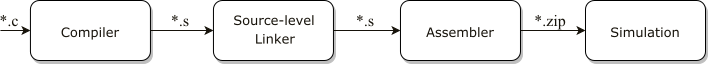
\includegraphics[width=.95\textwidth]{figures/linker_illustration1}
\caption{Workflow of simulation.}
\label{fig:linker_A}
\end{figure}

Doing the compilation and preprocessing steps from the compiler results in unlinked assembly code. Here symbols are not resolved yet, and it does not automatically generate a \emph{\_start} function. The source-level linker resolves the symbols and inserts a \emph{\_start} function in which the stack is initialized. However, the source-level linker works only for a single input file, therefore, all benchmarks are implemented in a single C file. The assembler and the simulator from the legacy toolchain are used and the source-level linker is necessary for the assembler to work. 

\begin{figure}[t]
\centering
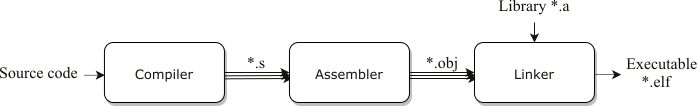
\includegraphics[width=.9\textwidth]{figures/linker_illustration2}
\caption{Standard linking process.}
\label{fig:linker_B}
\end{figure}

Figure \ref{fig:linker_B} illustrates the standard linking process when using the LLVM tools to do everything up to simulation. Other students have implemented an assembler and a linker within the LLVM framework. The assembler mainly consists of a parser that parses assembly code, and it uses LLVM-MC to form instructions to print them and the LLVM linker is developed within LLD. However, the new linker and assembler can not be used yet because it is still a work in progress.

%TODO: laat laatste 2 zinnen weg en voeg laatste zin uitgebreid toe



%Implementation of explicit datapaths using bypass registers.

%TODO: decide: comment or uncomment following section expl bp pass
%\subsection{Explicit Bypass Registers}
%This component implements the pass that we discuss in Section \ref{sec:expl_bp_impl} and thereby, implements the main goal of this project. It allocates explicit bypass registers on a machine function and it does that on a per basic block fashion using information of the pipeline state of other basic blocks. It uses \emph{BypassState} which keeps track of the bypass state of each basic block and can be configured to work on a given input state. This way the state of a pipeline can be analysed and remembered by the \emph{SimdExplicitRegister} pass after execution a basic block.

%\subsection{Instruction Printer}

%END COMPONENT DESCRIPTION

%\subsection{Assembler and Disassembler}



%Hier komt de uitleg v/d compiler implementatie en design. Bespreek hier eventuele tradeoffs die ik ben tegengekomen en design decisions die ik of anderen gemaakt hebben. Aangezien dit grotendeels een software project is, zou ik hier ook wat aandacht willen besteden aan software details, als in, bachelor software engineering skills erop los laten.  

%\Blindtext

\section{Exploiting Explicit Data Paths}\label{sec:expl_bp_impl}
%TODO: (OPTIONAL) move this to 3.3, and vice versa.
We exploit explicit data paths by going through the code and allocate these special bypass registers as a post processing step, in the sense that we do this after scheduling, register allocation, packetizing, etc. 
Doing this as a post processing step has advantages compared to doing this early on. 
\begin{enumerate}
\item When this is done before the packetizer, we would need to model the behaviour of the packetizer in this pass. Because this further complicates our implementation, we moved it to after the packetizer.
\item Another reason to do bypass allocation as a post processing step is because doing it at an earlier stage, where the code is not certain yet, gives more problems. Each of the custom passes may reorder or insert instructions, that would invalidate any bypass that were already allocated before that point.
\end{enumerate}

That being said, we have developed a class, called \texttt{BypassState}, which should be inherited by a class for each pipeline that we support, e.g. four and five stage pipeline. It models the values of busses that are in a pipeline, which we exploit for explicit data paths. %It keeps track of values that reside in those busses which keeps track of the . We have This that can be 

\begin{figure}[t]
\centering
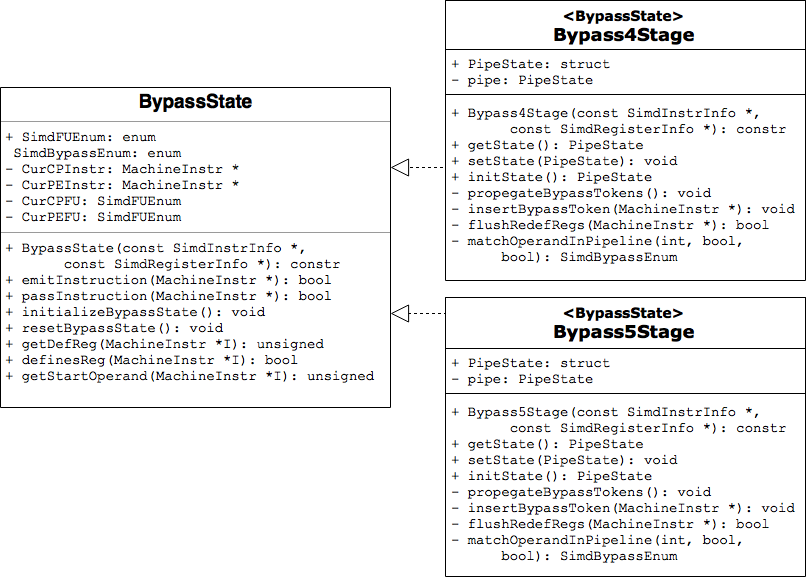
\includegraphics[width=\textwidth]{figures/class_diag_bpstate}
\caption{Class diagram for BypassState, and the inherited classes for the four and five state pipelines.}
\label{fig:class_diagram_bpstate}
\end{figure}

We give a class diagram for \texttt{BypassState} in Figure \ref{fig:class_diagram_bpstate}. Here we have the classes  \texttt{Bypass4State} and \texttt{Bypass5State} that represent the derived classes for the four stage and five stage pipeline respectively. Here we pass the operations as tokens to \texttt{BypassState} one at a time and propagate the tokens each cycle. There is a variable in the derived classes, called \texttt{pipe} which represents the instructions that are currently in our pipeline. The pipeline state can be queried at any giving moment using function \texttt{getState}. This function can be used to acquire the state just before a jump or at the end of a basic block.

Furthermore, functions \texttt{getDefReg} and \texttt{definesReg} can be used to determine what is written to the register file by an operation, and \texttt{getStartOperand} may be used to see where in an operation we need to start with bypassing RaW dependencies. Function \texttt{matchOperandInPipeline} from the derived classes can be used to see if we can exploit one of the busses in a pipeline. We model these busses with a structure, called \texttt{PipeState}. Table \ref{table:pipe_state} shows which variables it represents.

\begin{table}[H]
\caption{Representation of struct PipeState.}
\begin{center}
\begin{tabular}{@{}l l@{}}
\toprule
\textbf{Type} & \textbf{Variable} \\
MachineInstr* 	& Pipeline[N\_FUNCTION\_UNITS][N\_PACKET\_COUNT][EX\_STAGES]\\
MachineInstr* 	& WB[N\_PACKET\_COUNT]\\
SimdFUEnum	& issues[N\_PACKET\_COUNT][EX\_STAGES]\\
{\small *: pointer}\\
\bottomrule%%\\
%{\small * pointer}
\end{tabular}
\end{center}
\label{table:pipe_state}
\end{table}%

%This is where I will cover the software details and throw in some UML diagrams.
%\blindtext

\subsection{Approaches}\label{sec:approaches}
This is just a placeholder.

%TODO: add scheduler/before RA/combined scheduling&RA/group instructions together to increase number of bypasses/ etc.
 

\subsection{Software Design}\label{sec:explicit_impl}
%First, make the design space as large as possible
% tradeoffs/considerations/selection
% 1 or 2 solutions

%\begin{figure}[t!]
%\centering
%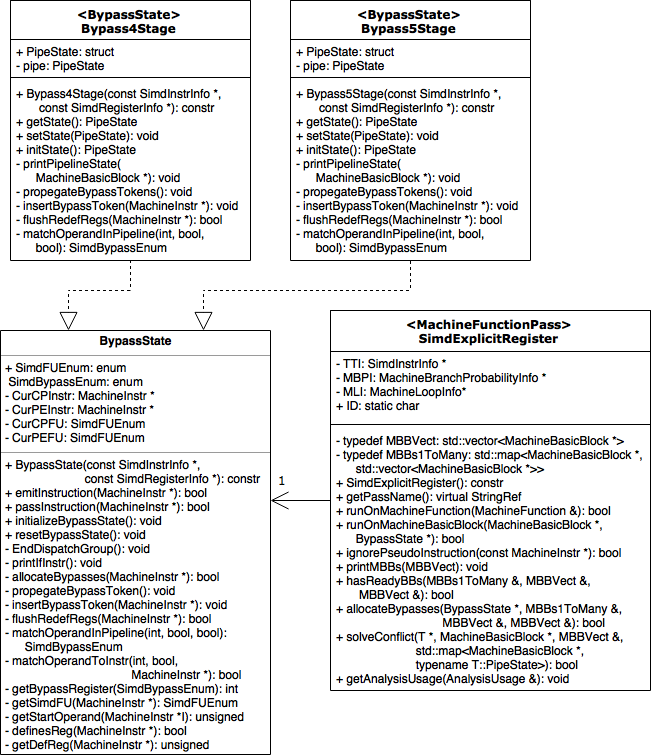
\includegraphics[width=.9\textwidth]{figures/class_diagram}
%\caption{Class diagram of the implemented approach to support explicit datapaths.}
%\label{fig:class_diagram}
%\end{figure}

There is a class called \texttt{BypassState} which should be inherited by each pipeline that we support, e.g. four-stage and five-stage pipeline. It models the values on busses in the bypass network. %It keeps track of values that reside in those busses which keeps track of the . We have This that can be 

\begin{figure}[b!]
\centering
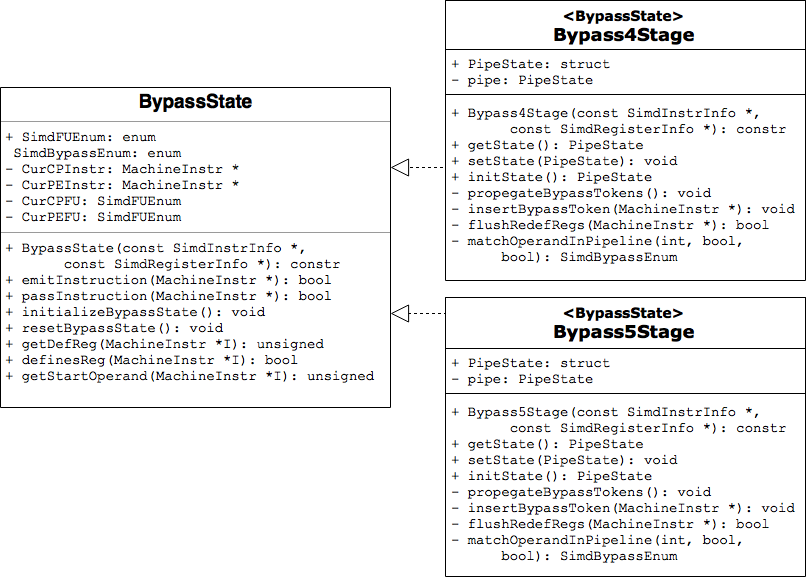
\includegraphics[width=\textwidth]{figures/class_diag_bpstate}
\caption{Class diagram for BypassState, and the inherited classes for the four-stage and five-stage pipelines.}
\label{fig:class_diagram_bpstate}
\end{figure}
%TODO: add following : there was a lot of functionality between the five stage pipeline and four-stage, so we define all shared functionality in \texttt{BypassState}, and stuff specific for a stage in \texttt{BypassXStage}.

We give a class diagram for \texttt{BypassState} in Figure \ref{fig:class_diagram_bpstate}. The classes  \texttt{Bypass4State} and \texttt{Bypass5State} represent the derived classes for the four-stage and five-stage pipeline respectively. Here we use \texttt{insertBypassToken} to pass the instructions in a basic block as tokens to \texttt{BypassState} one at a time and propagate the tokens each cycle using \texttt{propegateBypassTokens}. There is a variable in the derived classes, called \texttt{pipe} which represents the instructions that are currently in our pipeline. The pipeline state can be queried at any giving moment using function \texttt{getState}. This function can be used to acquire the state just before a jump or at the end of a basic block. The functions \texttt{initState} and \texttt{setState} may be used to initialize the state to a empty state, or a given state which is typically done at the beginning of a basic block. We use a function called \texttt{matchOperandInPipeline} to see what bypass can be allocated on a particular use operand of an instruction. It checks whether the operand uses a register defined by any of the instructions the pipeline (by calling \texttt{matchOperandToInstr} and \texttt{getDefReg} for each instruction can be forwarded). In general, it needs to find the newest definition of the register under consideration, therefore, when inserting a bypass token in the pipeline state we remove all occurrences using \texttt{flushRedefRegs}. This way we never have more than one instruction in the pipeline that define the same register, and thus always find the newest definition, if any.

Now lets continue with functions that handle instructions which are used to emit, pass or check an instruction (\texttt{emitInstruction}, \texttt{passInstruction} and \texttt{checkInstruction}). Emitting an instruction consists of the process of specifying which operations are in the current cycle and bypassing their operands according to the current pipeline state. Then pass instruction does the same, but the operands are not bypassed and check instruction does also not actually bypass the operands, but does keep the bypasses that it would allocate in a list. The functions \texttt{allocateBypasses} and \texttt{checkBypasses} do the actual bypassing work by calling \texttt{matchOperandInPipeline} which compares each operand of an instruction to  that can be bypassed. However, there are also flag operands that we do not consider. 
%\lstset{style=customasm}
%TODO: do something cool on the vector slots 
%\vspace{12px}
\begin{lstlisting}
    %loop
        sfgts r2, -64    || v.sfltu   P1, r1, 4
        bf    %loop      || v.slli.P1 r2, r1, 2
        add   r2, r2, -1 || v.add.P1  r7, r6, r2 
    %end:
                         <@\hspace{4px}$\vdots$@>
\end{lstlisting}

%TODO: move next paragraph to above listing, and remove newline
Flag operands occur before register source operands. The code fragment above shows an example of predicate instructions that uses flag operands to either do or not do a certain operation. In this case, we do a shift and add it with something if PE index is smaller than four ($P1$ is true). The function \texttt{getStartOperand} is used to skip flag operands. Alternatively we could also just ignore an operand if it is a flag operand. \\

After each cycle, a call is made to \texttt{EndDispatchGroup} which calls \texttt{insertBypassTokens} for each instruction in the current dispatch (can be two operations, a scalar and a vector op) and propagate the bypass tokens. So to summarize, operands are bypassed when they come across, and at the end of each cycle the pipeline is updated. %Meanwhile using getDef skip all instructions that occur but do not define an instruction. 


%TODO: verify and uncomment
%  later functions do not allocate bypass registers but may be used to insert instructions in the bypass state model, or to check which bypasses would be allocated according to a given bypass state (using \texttt{checkBypasses}), while the first one (\texttt{emitInstruction}) inserts the instruction into the bypass state model and allocates explicit bypasses wherever possible using \texttt{allocateBypasses}.


%TODO: verify and uncomment
% functions \texttt{getDefReg} and \texttt{definesReg} can be used to determine what is written to the register file by an operation, and \texttt{getStartOperand} may be used to see where in an operation we need to start with bypassing RaW dependencies. Function \texttt{matchOperandInPipeline} from the derived classes can be used to see if we can exploit one of the busses in a pipeline. We model these busses with a structure, called \texttt{PipeState}. 

%\begin{table}[b]
%\caption{Representation of struct PipeState.}
%\begin{center}
%\begin{tabular}{@{}l l@{}}
%\toprule
%\textbf{Type} & \textbf{Variable} \\
%MachineInstr* 	& Pipeline[N\_FUNCTION\_UNITS][N\_PACKET\_COUNT][EX\_STAGES]\\
%MachineInstr* 	& WB[N\_PACKET\_COUNT]\\
%SimdFUEnum	& issues[N\_PACKET\_COUNT][EX\_STAGES]\\
%{\small *: pointer}\\
%\bottomrule%%\\
%%{\small * pointer}
%\end{tabular}
%\end{center}
%\label{table:pipe_state}
%\end{table}%


%\clearemptydoublepage

%TODO: rewrite our solution and design options and tradeoffs and software architecture
%\chapter{Proposed Solution}\label{chapter:solutions}
%Our approach to implement explicit bypassing to fit it in our compiler within LLVM is to allocate the available bypasses sources during one of the compiler stages. The major compilation phases in LLVM are illustrated in Figure \ref{fig:phase_ordering}.  The first block represents instruction legalization, instruction lowering and instruction selection, In general, we have that first the instructions are scheduled, then register allocation (RA) is performed, and finally the instructions are printed in assembly language. Although one can use a post-RA scheduler to change the order in which to do scheduling and register allocation. At some point, we have to allocate our bypasses, which we can do only after we have backend specific instruction, i.e. after instruction selection. However, we could do this during any of compilation stages that follow, i.e. before scheduling and register allocation, during scheduling and register allocation and at the end of compilation. Moreover, scheduling and register allocation is already a phase problem on its own, as we have mentioned in Chapter \ref{sec:scheduling_and_ra}. Altogether, this leads to many possible approaches and we will discuss some of them below.

\begin{figure}[H]
\centering
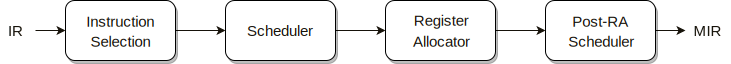
\includegraphics[width=.15\textwidth]{figures/phase_ordering}
\caption{Generalized code generation sequence.}
\label{fig:phase_ordering}
\end{figure}

\section{Last-minute Allocation}\label{sec:last_minute_alloc}
%Approach 1
One approach would be to allocate bypasses during the last stage of the compiler, just before printing the instructions. At this point, instructions are in order of execution and register allocation has already been performed and spill code has already been inserted in case we ran out of registers during RA. Because the order of instructions does not change at this point, the advantage of this approach is its simplicity. Namely, we could implement a pass that works on basic blocks, a basic block is a sequence of instructions with no branches, except for entering and leaving the basic block.

We could implement a pass to our backend that keeps track of the state of our pipeline in order to allocate our bypasses. Then we can determine for a cycle, which values currently reside in our bypass registers. Using this information we can then allocate bypasses andprocess the instructions in a top-down approach, demoting physical registers into bypass registers.

However, when we ran out of registers during register allocation, we had inserted spill code. When we allocate bypasses, we effectively free up registers. Since the spill code had already been inserted, it might have become unnecessary. Therefore, one improvement to this approach would be to move spill code after bypasses have been allocated to where they are needed, in order to avoid unnecessary spills.

\section{Bypass-aware Register Allocation}\label{sec:ra_approach}
%Approach 2
Another approach would be to implement a bypass-aware register allocator. Assuming that we have performed scheduling before register allocation, the instructions are in order of execution, allowing us to model the pipeline state as we did for the first approach. Our bypass-aware register allocator could start by allocating bypass registers. Then the remaining virtual registers could be allocated as usual. With this approach, we reduce register pressure by allocating bypasses before register allocation, effectively freeing registers. Therefore we may need less spill code, which is now inserted after bypasses have been allocated. So in contrary to the first approach, we do not have to take special care of spilling.

This approach would require us to implement a custom register allocator that consists of two phases. First, we allocate a bypass registers for each virtual register that can be bypassed. Subsequently, we have to allocate physical registers for the remaining virtual register. For the second phase we may reuse any of the existing register allocators. 
%Introduce example code where we could have better bypass utilizzation, i.e. less stores by scheduling differently

\section{Bypass-aware Scheduling}\label{sec:scheduling_approach}
%Approach 3
For this approach we need to implement a custom scheduler for our backend. This scheduler would prioritize to schedule instructions that may be bypassed close to each other, such that we may increase the possible number of bypasses. If we were to allocate bypasses during scheduling, code might be inserted during register allocation or any other passes that follow, that may break a previously allocated bypass. Therefore, it may be wise to allocate the bypasses as late as possible, and let the scheduler be responsible for improving utilization of the bypass network. 


\section{Pre Scheduling Allocation}\label{sec:pre_scheduling}
%Approach 4
Before scheduling, we can identify instruction pairs that we can bypass. Then we change the virtual register that is bypassed into bypass registers and glue the two instructions together. This however makes restrictions on the resulting schedule. Since we group instruction together before scheduling, we may improve utilization of the bypass network. Namely, we may have grouped instruction together that otherwise would be scheduled far apart. This approach requires some new heuristics to determine whether it is profitable to group instruction together or when this may decrease efficiency, i.e. when grouping instructions decreases available ILP. 

When we allocate bypasses before scheduling and register allocation, it is possible that the scheduler or register allocator reorder instruction, or insert instruction, e.g. spill code, which breaks a previously allocated bypass. Therefore, a better approach would be to group instructions together as explained above, but allocate the bypasses as late as possible, similar to the previous approach.

With this approach, we would need to find a tradeoff to not restrict the schedule too much, but still utilizing the bypass network as much as possible.   

\section{Combined Scheduling and Register Allocation}\label{sec:combined_sched_ra}
%Approach 5 & 6
We can also choose to solve scheduling and RA in one go. This way, problems that can arise of doing one before the other may be avoided. There are two approaches to solve this problem. One is to solve it optimally, using constraint programming. Unison, a separate project that solves scheduling and register allocation optimally in one go can be used with LLVM and can be extended to allocate our bypasses. However, solving this problem optimally, may increase compilation time significantly, which we would like to avoid. Therefore, another approach would be to use heuristics to solve scheduling and register allocation in one go. There are no implementations of this thus far, which makes this approach the most difficult one. However, when we can efficiently deal with these problems in one go, we might extend this for other architectures as well. 

%\clearemptydoublepage

% TODO: collect data for graphs / effectiveness / code quality en dergelijke
\chapter{Evaluation}\label{chapter:evaluation}
%TODO: add list of benchmarks, each with explanation and charactaristics.
%Add picture of complete toolflow (from C to estimates).
%Add results section,
%Add discussion on results

In order to evaluate the performance of the compiler, a set of benchmarks is used. The assembly code generated by the two compilers will be compared on `code quality' and on the number of register reads and writes it can avoid by exploiting explicit datapaths. To verify correctness of the generated code, the simulation output of the code generated by the LLVM compiler and of the code produced by the legacy compiler are compared to a reference. The references are generated using GCC\footnote{gcc.gnu.org} and the result of GCC is an executable that prints the reference output upon execution. This reference output is compared to the simulation results and if they match, the compiler can generate a correct code.

To compare the two compilers, scalar-only code is considered such that the comparison is fair. Then the auto-vectorizer is enabled for further analysis which results in more efficient code. This in turn is compared to handwritten assembly code to see how efficient the generated code truly is.

\section{Benchmarks}
The collection of benchmarks is presented in Table \ref{table:benchmarks_overview}. Originally there are more benchmarks apart from these, but they are left out because they are part of, or too similar to another benchmark. Furthermore, there is not a handwritten reference for each of these benchmarks. Namely, only \emph{binarization}, \emph{color conversion} and \emph{convolution} have vectorized assembly code references. From these references \emph{binarization} and \emph{convolution} have been handwritten by L. Waeijen, and \emph{color conversion} is vectorized by the legacy compiler using OpenCL code.

\begin{table}[H]
\caption{List of benchmarks.}
\begin{center}
\begin{tabular}{@{}l l l l@{}}
\toprule
\textbf{Benchmark} 	& \textbf{Comments} & \hspace{-30px}\textbf{Complexity}	 		\\ \hline
Addition			& Sums the individual elements of matrix $A$ and $B$.	& -- --\\
Binarization		& Converts a pixel image to a binary image. 			& --\\
Convolution		& Adds each pixel to its local neighbors, weighted by a kernel. & ++\\
DES				& A symmetric-key algorithm for encryption of data. 		& ++	\\
Histogram			& Plots the frequency distribution of a data set. 			& +\\
Matrix Multiplication	& Multiplies matrix $A$ and $B$ to form matrix $C$. 		& +\\
Matrix Transpose	& Calculates $A^T$ by reordering each row.			& +/--\\
YUV2RGB		& Color conversion to transform a YUV image to a RGB image.	& +\\
\bottomrule
\end{tabular}
\end{center}
\label{table:benchmarks_overview}
\end{table}%

\newpage

\begin{table}[t]
\caption{Summarizes which of the benchmarks have been vectorized and provides an overview of how many cycles were additionally executed because of instructions inserted by Section \ref{sec:conflicts} for both scalar- and vector-version, and how many cycles were additional executed with explicit bypassing for the legacy compiler.}
\begin{center}
\begin{tabular}{@{}l l c c c@{}}
\toprule
\textbf{Benchmark} 	& \textbf{Vectorized} & \multicolumn{3}{@{}c@{}}{\textbf{Additional cycles exec.}}	\\
				& 				& \textbf{(legacy)}	& \textbf{(scalar)} 	& \textbf{(vector)}	\\ \hline
				&				& 4st./5st.			& 4st./5st.			& 4st./5st.			\\
Addition			& Yes			& 1/2				& 0/0				& 0/0				\\
Binarization		& Yes			& 0/0				& 1/2				& 1/2				\\
Convolution		& No				& 33/32			& \ 4000/15432		& -				\\
DES				& No				& 351/367			& \ \ \ 1/770		& -				\\
Histogram			& Yes*			& 0/2				& 0/0				& 257/130\ 		\\
Matrix Multiplication	& Yes			& 0/0				& 8/2				& 1/4				\\
Matrix Transpose	& Yes*			& 0/0				& 1/0				& 1/2				\\
YUV2RGB		& Yes			&\ 0/48			& 0/0				& 1/4				\\ %TODO: determine ?
\multicolumn{5}{@{}l@{}}{\small - N/A.}\\ 
\multicolumn{5}{@{}l@{}}{\small * vectorized, but less efficient than scalar version.}\\ 
\bottomrule
\end{tabular}
\end{center}
\label{table:benchmarks_summary}
\end{table}%


%TODO: verify and rewrite this part and fill/collect future work.
The \emph{Data Encryption Standard} (DES) benchmark has not been vectorized because of irregular memory accesses. For other benchmarks e.g. \emph{histogram} and \emph{matrix transpose}, vectorization results in less efficient code. This is often caused by neighborhood network communication which is expensive for the target architecture.

%TODO: ADD PROBLEM OF CONVOLUTION VECTRIZATION, namely !! REDUCTION !!
\emph{Convolution} has not been vectorized because of an open issue with vectorized kernels that use reduction. The \emph{binarization} and \emph{YUV2RGV} benchmarks had some difficulties during vectorization because of a compilation problem when multiple set-flag and conditional move operations are present in a generated code. Problems like these and others are described in the future work section in Chapter \ref{chapter:conclusion}. In overall, the vectorized versions perform better with a speedup of ... \%. The vectorized versions are compared to scalar-only code and with the legacy compiler in Figure \ref{fig:total_domination}.


\section{Legacy Compiler Results}

\begin{figure}[b!]
\centering
\hspace*{-.12in}
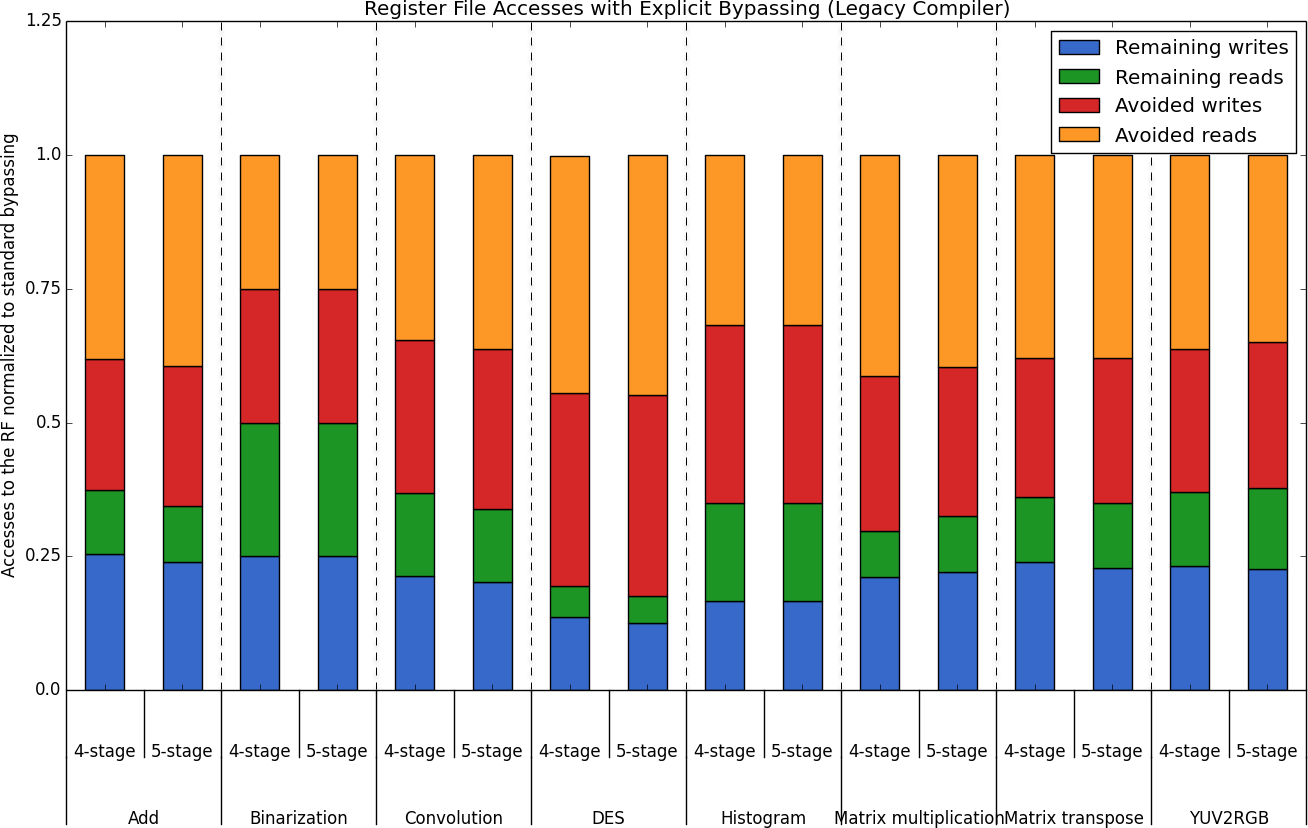
\includegraphics[width=\textwidth]{figures/stats/legacy_accesses}
\caption{Register file accesses with explicit bypassing on the legacy compiler (accesses are normalized to the total number of accesses with automatic bypassing (with an overall improvement of 70\% on writes and 56\% on reads). Note that the automatic bypass version does not avoid any write accesses, however it does avoid some read accesses.}
\label{fig:legacy_access_improvements}
\end{figure}




\section{Scalar Version Comparison}
This section compares the legacy compiler to the current compiler (Figure \ref{fig:legacy_scalar_cmp}).  

\begin{figure}[t!]
\centering
\hspace*{-.12in}
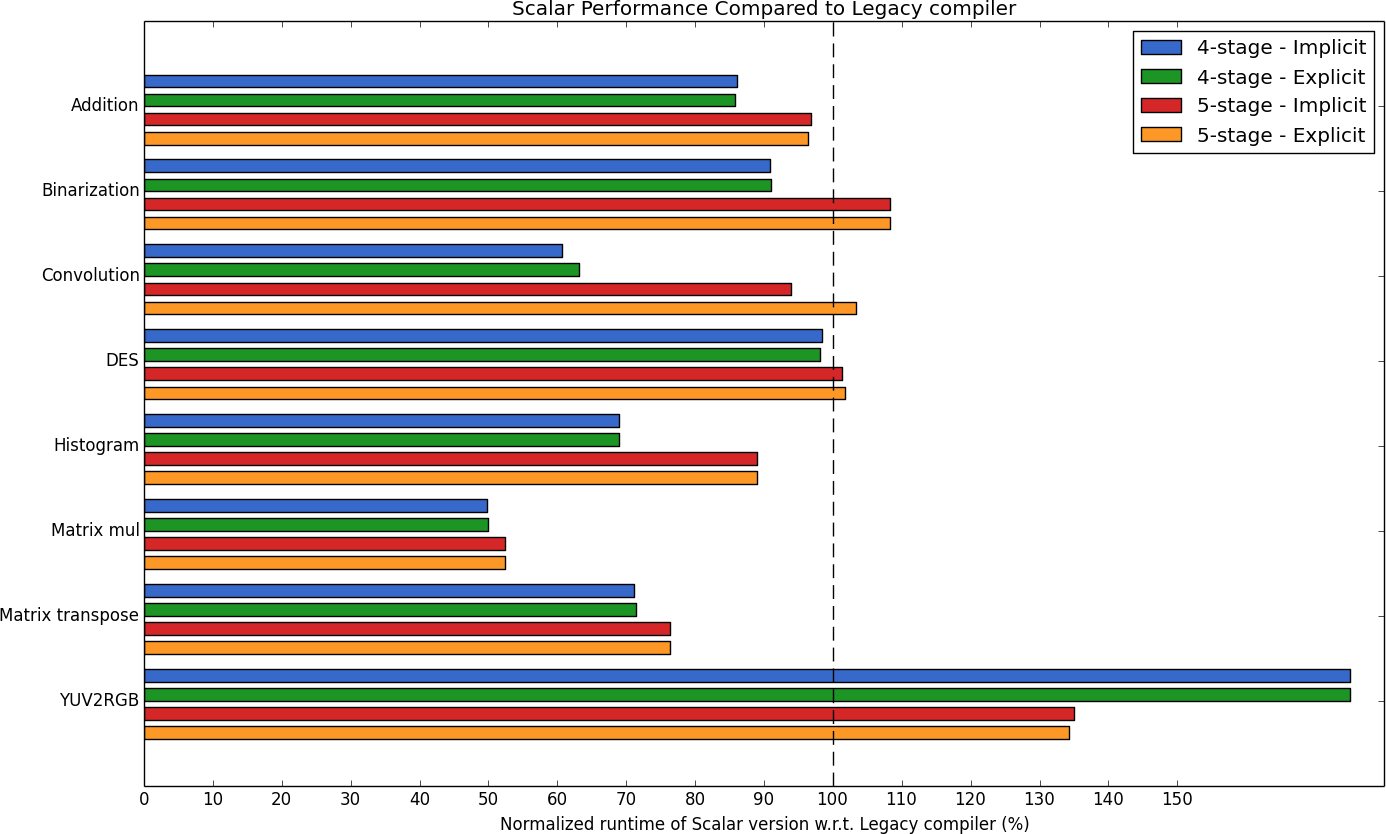
\includegraphics[width=\textwidth]{figures/stats/scalar_cycles}
%TODO: change orange to yellow and yellow to orange in picture. 
\caption{Scalar version performance comparision (cycle counts are normalized to that of the legacy compiler), with an average improvement of over 28\% in terms of cycles.}
\label{fig:legacy_scalar_cmp}
\end{figure}

%LALALALA lele

Figure \ref{fig:legacy_access_improvements} or Figure \ref{fig:legacy_write_impr} and Figure \ref{fig:legacy_read_impr}.

%%TODO rEMOVE THIS NEWPAGE
%\newpage
%%END TODO

Figure \ref{fig:scalar_improvements} shows a bar chart with how many register file accesses can be avoided by the new compiler where the accesses are normalized to automatic bypassing. The optimizations for this picture include using a scheduler optimization flag \texttt{-misched-nolimit=1} to not schedule too far, and optimization level \texttt{-O2}. The instructions are scheduled closer to their use by not buffering instructions during scheduling. The difference in the total number of cycles does not differ compared to \texttt{-O2} with no other optimization flags, but does give a overall better improvement on accesses to the RF with an average of around 60\% on register writes and 40\% on RF reads.\\

Add example \\ %Use closer to def with -misched-limit=1.



\begin{figure}[b!]
\centering
\hspace*{-.12in}
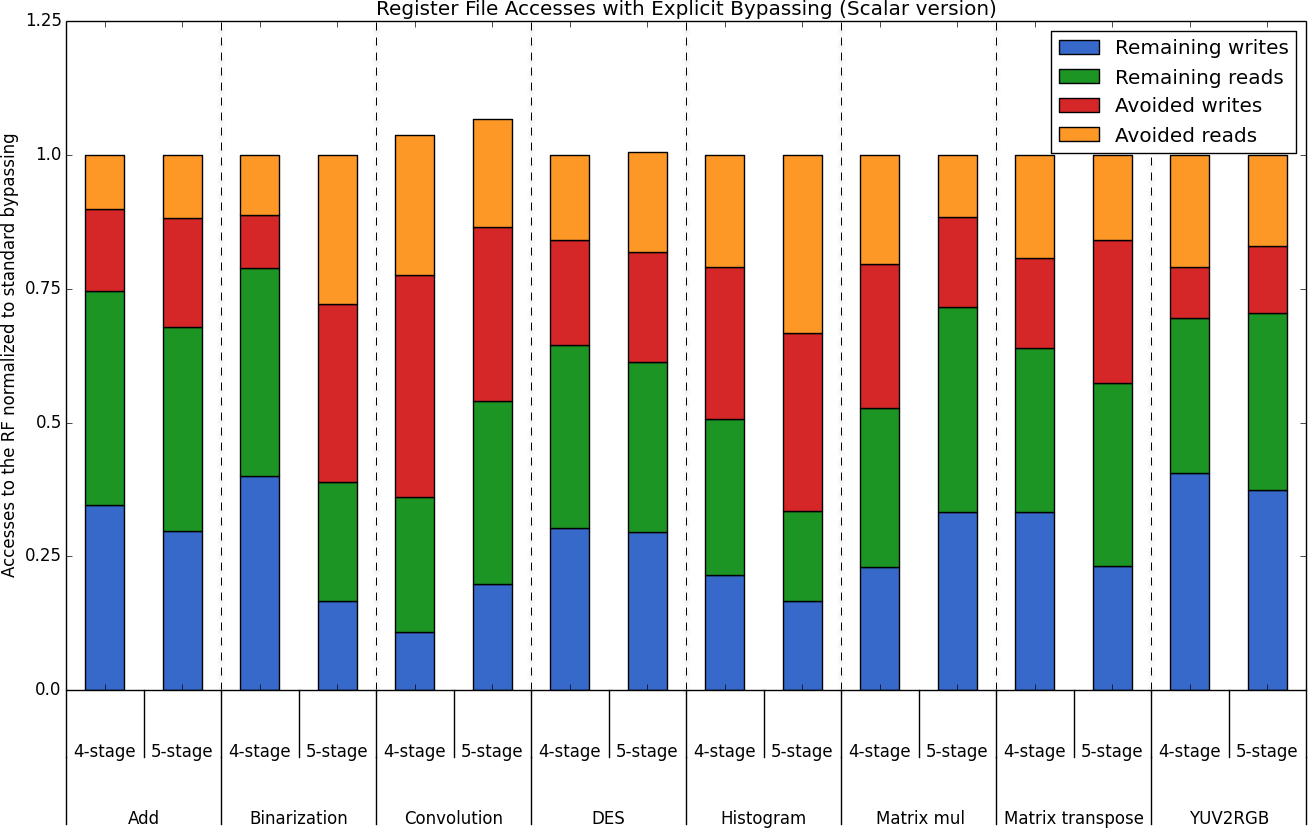
\includegraphics[width=\textwidth]{figures/stats/scalar_accesses}
%TODO: change orange to yellow and yellow to orange in picture. 
\caption{Scalar version register accesses (RF accesses are normalized to implicit bypassing), with an average improvement of over 56\% on writes and 40\% on reads.}
\label{fig:scalar_improvements}
\end{figure}



\begin{figure}[H]
\centering
\hspace*{-.12in}
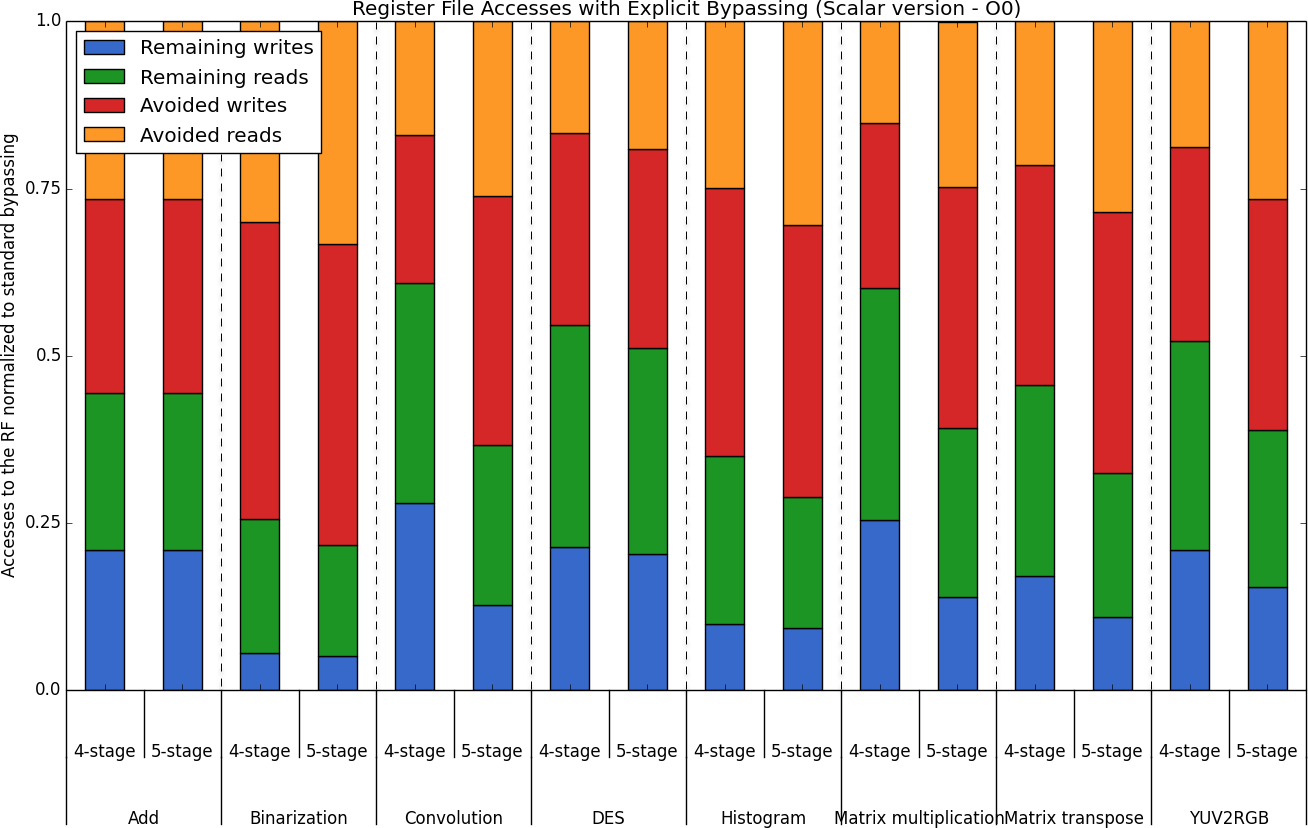
\includegraphics[width=\textwidth]{figures/stats/scalar_accesses_O0}
%TODO: change orange to yellow and yellow to orange in picture. 
\caption{Scalar version register accesses with opt-level \texttt{-O0} (RF accesses are normalized to implicit bypassing), with an average improvement of over 77\% on writes and 54\% on reads.}
\label{fig:scalar_improvements_O0}
\end{figure}

With the lowest optimization level, the savings on the register file can go up to 77\% writes and 54\% on reads on average. With such low optimization level, the total number of cycles increases rapidly with an increase in cycles of up to 6-7 times (convolution). However, for some benchmarks, e.g. histogram, it still performs quite well with only a 50\% increase in cycles, while the increase in utilization of the bypass network is significant. Figure \ref{fig:scalar_improvements_O0} shows RF accesses with explicit bypassing, the lowest optimization level and scalar-only code. A large performance lost due to such low optimization level was found for all benchmarks, except for \emph{histogram} and \emph{binarization}. For these two benchmarks which execute in around 50\% more cycles, do have a significant result by avoiding up to almost all write accesses.

%OR 

%\begin{figure}[H]
%\centering
%\subfloat[Register write improvements normalized to automatic bypassing.]{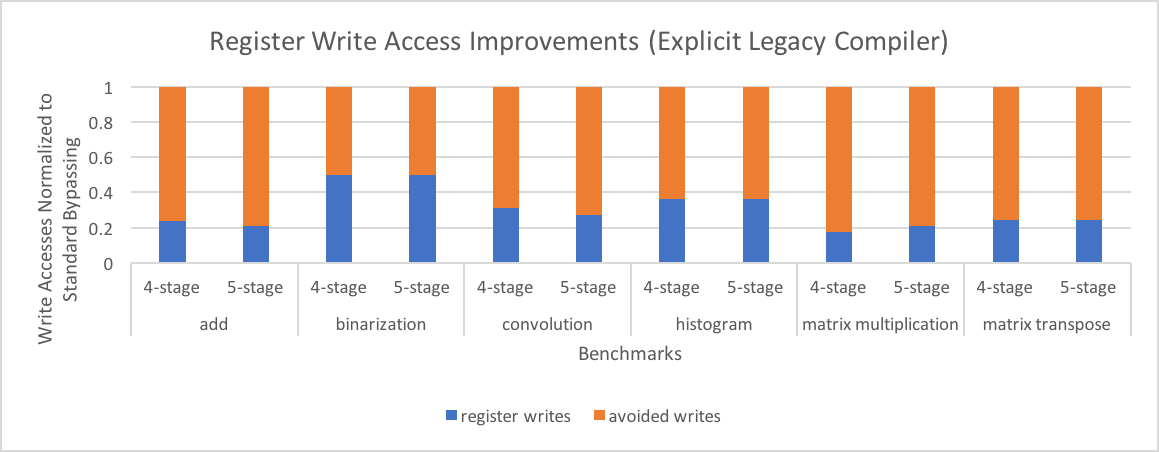
\includegraphics[width=.75\textwidth]{figures/stats/legacy_writes}%
%\label{fig:legacy_write_impr}}
%\hfil
%\subfloat[Register read improvements normalized to automatic bypassing.]{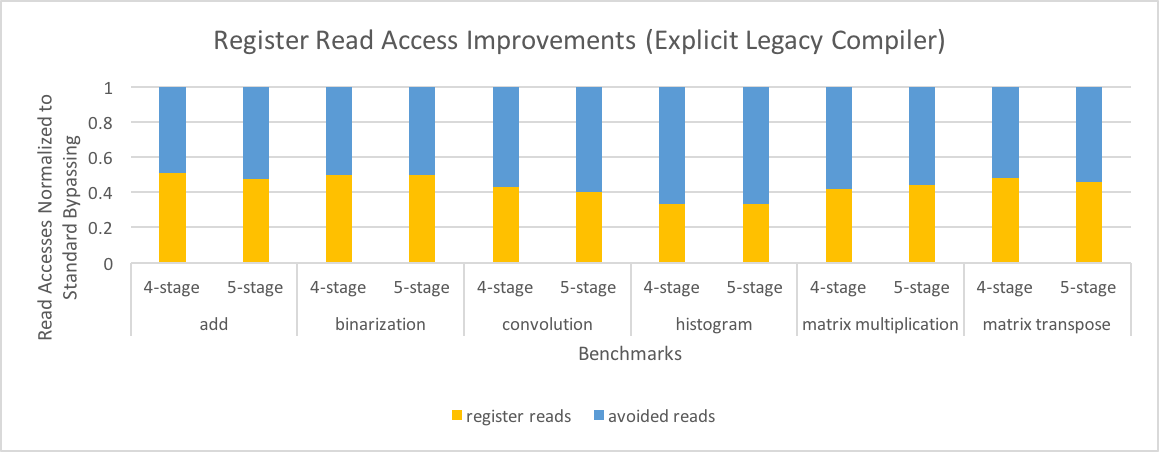
\includegraphics[width=.75\textwidth]{figures/stats/legacy_reads}%
%\label{fig:legacy_read_impr}}
%\caption{Gain in access to the bypass network, normalized to register accesses by the automatic bypass version. }
%\label{fig:legacy_access_improvements}
%\end{figure}

\section{Vector Version Comparison}

\begin{figure}[b!]
\centering
\hspace*{-.12in}
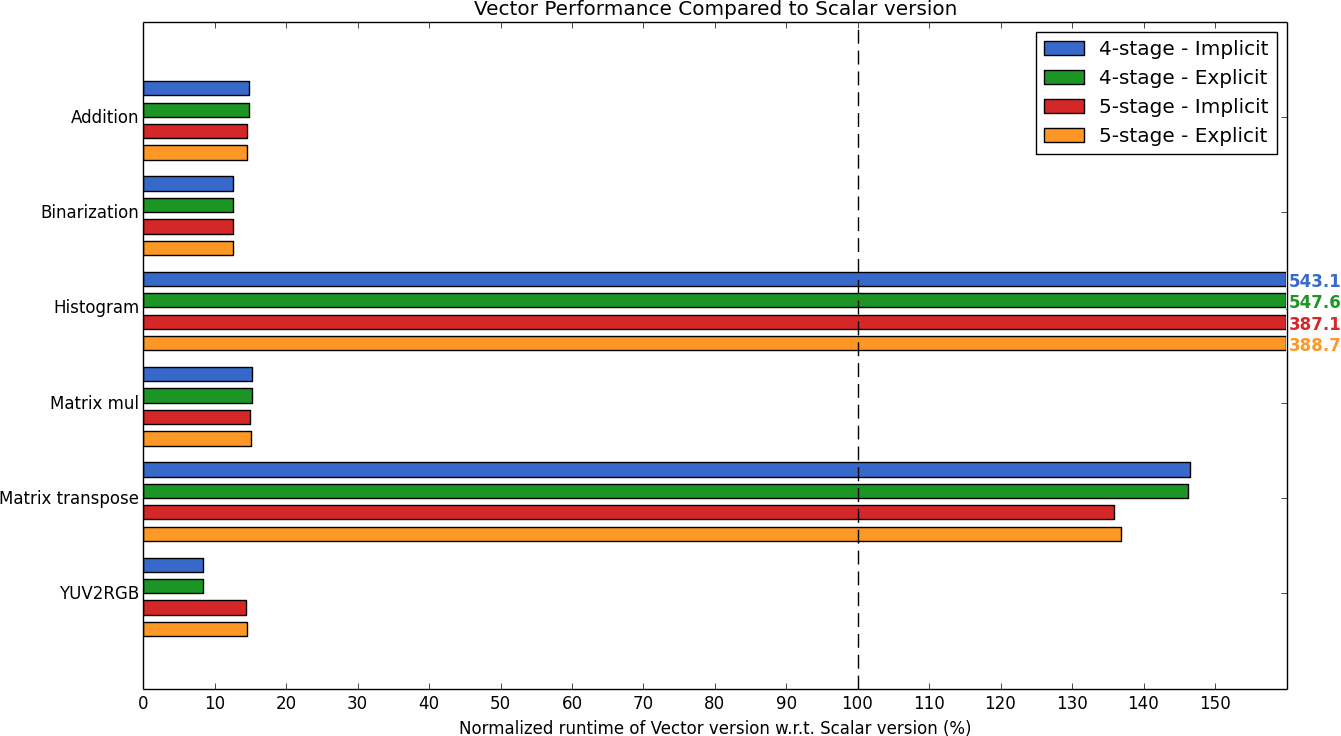
\includegraphics[width=\textwidth]{figures/stats/vector_cycles}
%TODO: change orange to yellow and yellow to orange in picture. 
\caption{Vector version performance gain (cycle counts are normalized to that of the legacy compiler), with an average improvement of 65 percent.}
\label{fig:vector_scalar_cmp}
\end{figure}


\begin{figure}[t!]
\centering
\hspace*{-.12in}
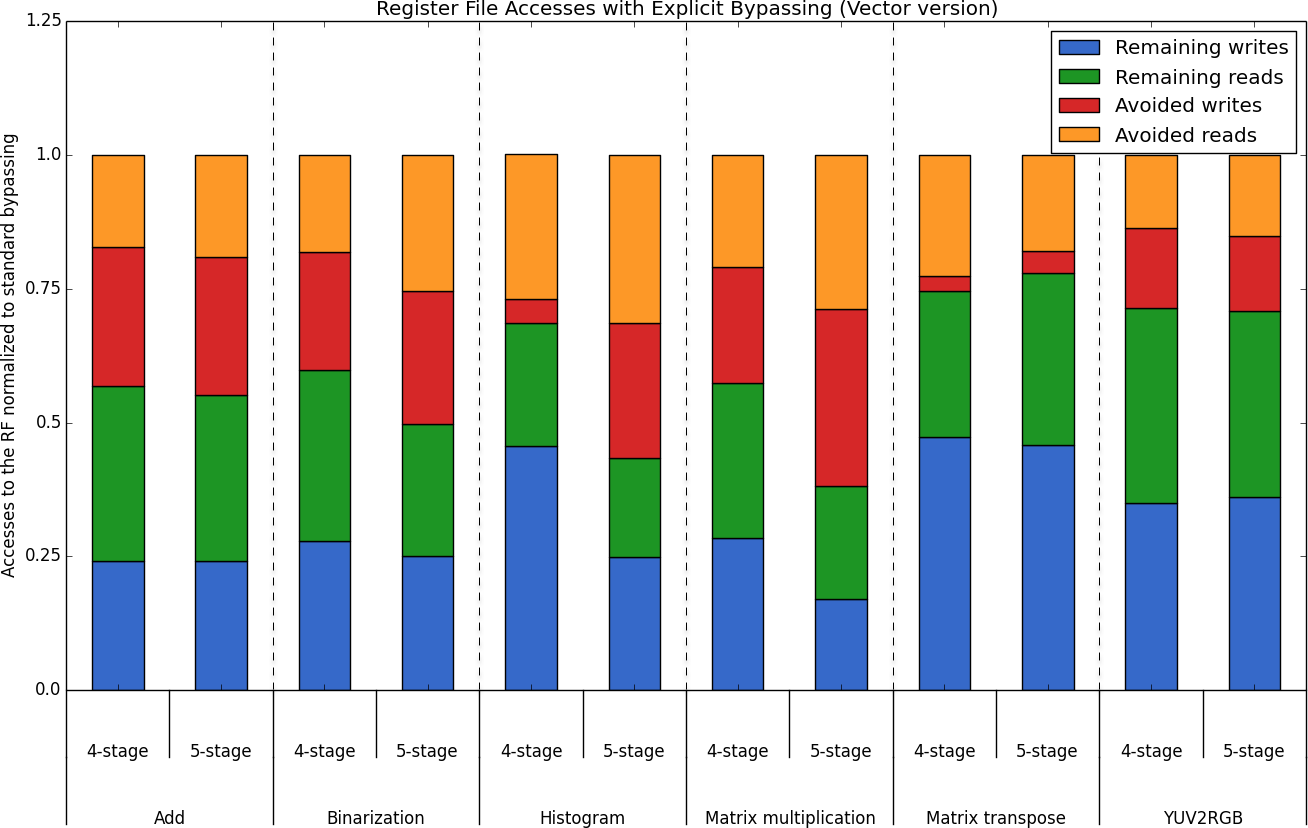
\includegraphics[width=\textwidth]{figures/stats/vec_accesses}
%TODO: change orange to yellow and yellow to orange in picture. 
\caption{RF accesses for the vector version, accesses are normalized to standard bypassing.}
\label{fig:vec_accesses}
\end{figure}


\newpage

Matrix mul benchmark, desired code. Give actual and then desired code! (that is the code below).



%TODO: discuss any inefficiencies here: 
%1: Inefficiencies by the source-level-linked, e.g. always zimm/simm in front of address to a global variable. 
%	This behaviour needs to be implemented by the standard linker too!

%2: Give one full application still needs to be done! :(
%3: discuss or at least think of a way to optimally reduce comm. using DDGs and traits


\begin{lstlisting}
A:
   addi r11, r11, -4 || v.addi r11, r11, -4
   sw   r10, r11,  0
   add  r10, r11, r0
B:
   lw   r1,  r10,  0
C:
   addi r3,  r0,   0 || v.addi r2,  r0,  16
   lw   r4,  r3,   0 || v.lw   r5,  r2,   0
   lw   r5,  r3,   1 || v.lw   r4,  r2,   1
   lw   r6,  r3,   2 || v.lw   r3,  r2,   2
   lw   r7,  r3,   3 || v.lw   r2,  r2,   3
D:
   addi r4,  r4,   0 || v.add  r6,  CP,  r0
   addi r5,  r5,   0 || v.add  r7,  CP,  r0
   nop               || v.mul  r6,  r5,  r6
   nop               || v.mul  r7,  r4,  r7
   nop               || v.add  r6,  r7,  r6
   addi r6,  r6,   0 || v.add  r7,  CP,  r0
   nop               || v.mul  r7,  r3,  r7
   addi r7,  r7,   0 || v.add  r8,  CP,  r0
   nop               || v.add  r6,  r7,  r6
   nop               || v.mul  r7,  r2,  r8
   nop               || v.add  r6,  r7,  r6
   addi r1,  r1,  -1 || v.addi r7,  r0,  32
   sfeq r1,  0       || v.sw   r6,  r7,   0
   bf   E
   nop
   j    C  
   nop
E:
   lw   r10, r11,  0
   addi r11, r11,  4 || v.addi r11, r11,  4
   jr r9
   nop
\end{lstlisting}

%\clearemptydoublepage

%======== step n - 1, write conclusions and discussion perhaps, also same content in presentation
\chapter{Conclusions}\label{chapter:conclusion}
The implementation of a SIMD compiler based on LLVM infrastructure has been described in the previous chapters. This chapters summarizes the results, shows the limitations of the compiler, and presents future work.

\section{Summary}
\Blindtext

\section{Future Work}\label{sec:future_work}
Optimalisaties en ander werk (e.g. disassembler) dat ik tegen kom, maar geen tijd voor heb om te implementeren/buiten de scope v/h project valt komt hier.

Als dit een klein hoofdstuk wordt (<2 paginas) dan kan deze worden samegevoegd met de Conclusie in Hoofdstuk \ref{chapter:conclusions}. 

\blindtext

\Blindtext



%In general a short summarizing paragraph will do, and under no circumstances should the paragraph simply repeat material from the Abstract or Introduction. In some cases it's possible to now make the original claims more concrete, e.g., by referring to quantitative performance results.

%Old text
%We have implemented last-minute bypass allocation and tested it on some benchmarks. However, we do not yet have all the benchmarks that we intend to use. Therefore we do not yet have reliable results that could indicate how efficient our first approach is. Furthermore, we have implemented last-minute bypassing for code generation, where we use only the CP processor. We want to extend this to allocate bypasses in a basic block for code generation, where we use both CP and PEs.

%The overall results are good, however, there are some limitations. Our approach processes basic blocks with only the available information of the current basic block. We notice that bypassing opportunities may be missed for small basic blocks, having only a few instructions. %This could be resolved however, by splitting the current pass in an analysis pass and a transformation pass. We then run the analysis part first, so that we have the state of 


%BEGIN PROS & CONS
%We have evaluated each of the proposed solutions on their tradeoffs in table \ref{table:tradeoffs} on estimated implementation effort, compilation times if the approach were used, and gain in code quality that we may expect for each of the solutions. 

%\begin{table}[h]
%\caption{Table with tradeoffs for each approach from Chapter \ref{chapter:solutions}.}
%\begin{center}
%\begin{tabular}{@{}p{0.4\textwidth-2\tabcolsep}p{0.2\textwidth-2\tabcolsep}p{0.2\textwidth-2\tabcolsep}p{0.2\textwidth-2\tabcolsep}@{}}
%\toprule
%\textbf{Aprroach} 		& \textbf{Implementation simplicity} & \textbf{Compilation speed} & \textbf{Quality of the compiled code} \\ \hline
%Last-minute Allocation  	& $++$ & $+$ & $+$ \\
%Bypass-aware Register Allocation & $+$ & $+$ & $+$ \\
%Bypass-aware Scheduling & $+$ & $+$ & $+$ \\
%Pre Scheduling Allocation & $-$ & $+$ & $+$ \\
%Combining Scheduling and Register Allocation Heuristic & $--$ & $+$ & $++$ \\
%Combined Scheduling and Register Allocation with Unison & $-$ & $--$ & $++$ \\
%\bottomrule
%\end{tabular}
%\end{center}
%\label{table:tradeoffs}
%\end{table}%

%\clearemptydoublepage

%======== step n, planning of what we did and when we did it, red line: 80% April till June & then full time onwards.
%\chapter{Planning}\label{chapter:planning}
%Coarse-grain and fine-grain planning for the graduation phase. The graduation phase will take six months, so we distribute that time span over each of the phases in Table \ref{table:planning}.

\begin{table}[h]
\caption{Time table for the graduation phase.}
\begin{center}
\begin{tabular}{@{}p{0.25\textwidth-2\tabcolsep}p{0.6\textwidth-2\tabcolsep}p{0.15\textwidth-2\tabcolsep}@{}}
\toprule
\textbf{Phase} 		& \textbf{Tasks} & \textbf{Duration} \\ \hline
Benchmarks setup 	& Develop benchmarks described in Chapter \ref{chapter:evaluation}.			& 1 week \\
First phase		& Implement a pass that allocates bypasses last minute, just before instructions are printed, as described in Chapter \ref{sec:last_minute_alloc}.		& 1 week \\
Second phase	& Implement a custom register allocation, that first allocates bypasses and allocates the remaining registers as usual, as described in Chapter \ref{sec:ra_approach}.	& 2 weeks \\
Third phase		& Implement a custom scheduler for our backend, that improves utilization of the bypass network, as described in Chapter \ref{sec:scheduling_approach}. & 3 weeks \\
Fourth phase 	& Implement a pass glueing instructions together that can be bypassed, as described in Chapter \ref{sec:pre_scheduling}. & 3 weeks\\
Fifth phase 	& Extend Unison to make it bypass aware, as described in Chapter \ref{sec:combined_sched_ra}. & 3 weeks \\
Sixth phase		& Implement heuristics that do combined RA and scheduling, as described in Chapter \ref{sec:combined_sched_ra}. & 5 weeks \\
Final report		& Write report and collect benchmark data. 	& 6 weeks \\
\hline%\cline{3-3}
\multicolumn{2}{c}{ \multirow{2}{*}{Total time}} 				& 24 weeks\\
	&											& (6 months)\\
\bottomrule
\end{tabular}
\end{center}
\label{table:planning}
\end{table}%
				

%\clearemptydoublepage

%Choose a good bibliography style, plain would do often, but these might be nice too
\bibliographystyle{ieeetr}
%\bibliographystyle{plain}
\bibliography{references}

%\clearemptydoublepage

%TODO: choose, with/without empty page with appendices, or just appendix, no newpage at end of document..
%begin{appendices}
\begin{appendices}
\chapter{Pseudo Code}\label{appendix:pseudo_code}
%Appendix C.

%TODO: mention that I left out CMakeFiles and LLVMBuildInfo for simplicity of the directory tree.
%\section{File Structure}
This appendix provides pseudo code of the pass that exploits explicit datapaths from Chapter \ref{sec:expl_bp_impl}. First of all, the children of each node in the dominator tree are sorted on reverse post-order tree traversel. Then each node and the functions \texttt{EnterScope} and \texttt{ProcessBlock} are called.\\

%TODO: add more introducing text, and explain pseudo code with text.
\begin{algorithm}[H]
 \KwData{PerformEBA}
 \KwResult{Explicit bypass allocation is performed}
 Sort dominator tree on reverse post order traversal\;
 
 Node = depthFirst(DominatorTree.root())\;
 \While{node}{
  block = Node.block()\;
  EnterScope(block)\;
  ProcessBlock(block)\;
  Node = next(Node)\;
 }
 \caption{Outer function called by \texttt{RunOnMachineFunction}.}
\end{algorithm}

\texttt{EnterScope} sets up the pipeline state by taking the bypass state from the most-frequently executed predecessor block. Subsequently, it modifies other predecessor blocks to match their resulting pipeline state when it is required by a bypass.\\

\begin{algorithm}[H]
 \KwData{EnterScope}
 \KwResult{Pipeline state is setup and conflicts on predecessors has been resolved}
 \eIf{isLoop}{
  \For{block in loop}{
   AnalyzeBlock(state, block)\;
  }
  setState(state)\;
 }{
  \eIf{preds.size() $>$ 1}{
   setState(MostFrequentlyExecutedPred.getState())\;
   checkConflicts(preds)\;
  }{
   \eIf{preds.size $==$ 1}{
    setState(pred.getState())\;
   }{
       initState()\;
   }
  }
 }
 \caption{First function called by \texttt{PerformEBA}.}
\end{algorithm}



\newpage



Where \texttt{AnalyzeBlock} goes through a basic block, and updates the pipeline state model accordingly. The procedure calls to \texttt{setState} and \texttt{getState} set the pipeline state model to a given state, or queries the pipeline state model of a basic block. The following pseudo code shows functionality of \texttt{ProcessBlock}, which is similar to \texttt{AnalyzeBlock}, but also allocates explicit bypasses that it finds.

\begin{algorithm}[H]
 \KwData{ProcessBlock}
 \KwResult{Explicit bypass allocation is performed on a basic block}
 \For{instruction in block}{
  allocateBypasses(instruction)\;
  
  insertIntoPipeline(instruction)\;
  register instruction in pipeline state model\;
  \If{end cycle}{
   propagate pipeline state\;
  }
 }
 \caption{Second function called by \texttt{PerformEBA}.}
\end{algorithm}

\begin{algorithm}[H]
 \KwData{allocateBypasses}
 \KwResult{Explicit bypass allocation is performed on an instruction}
 \For{operand in instruction}{
  match = matchOperandInPipeline()\;
  \If{match}{
   bypass operand\;
  }
  \If{match $\And$ isKill}{
   avoid store\;
  }
 }
 \caption{Inner function called by \texttt{ProcessBlock}.}
\end{algorithm}
\chapter{Instruction Set Architecture}\label{appendix:isa}
%TODO: verify descriptions with Liu's thesis

This appendix contains descriptions of the instructions that are supported on the proposed SIMD architecture. We have split the instructions into three classes, Register-type instructions that take only registers as operand. Immediate-type instructions have an immediate value as last operand. Finally, Jump-type instructions are instructions that modify the program counter.

\section{Register-type Instructions}
\begin{table}[h]
\begin{center}
\begin{tabular}{@{}p{0.1\textwidth-2\tabcolsep}p{0.15\textwidth-2\tabcolsep}p{0.1\textwidth-2\tabcolsep}p{0.65\textwidth-2\tabcolsep}@{}}
%\begin{tabular}{| c | c | c | l |}
\toprule
\textbf{Opcode} & \textbf{Operation} & \textbf{FU} & \textbf{Description}\\ \hline
0 & N/A & N/A		& Not used. \\ 
1 & N/A & N/A		& Not used. \\ 
2 & add & ALU		& Signed addition. \\ 
3 & sub & ALU		& Signed subtraction. \\ 
4 & mul & MUL	& Signed multiplication. \\ 
5 & mulu & MUL	& Unsigned multiplication. \\ 
6 & or & ALU		& Zero extended bitwise or. \\ 
7 & and & ALU		& Zero extended bitwise and. \\ 
8 & xor & ALU	& Zero extended bitwise xor. \\ 
9 & cmov & ALU	& Conditional move. \\ 
10 & sfeq & ALU	& Set flag if equal. \\ 
11 & sfne & ALU	& Set flag if not equal. \\ 
12 & sfles & ALU	& Set flag if less or equal, signed. \\ 
13 & sflts & ALU	& Set flag if less, signed. \\ 
14 & sfges & ALU	& Set flag if greater or equal, signed. \\ 
15 & sfgts & ALU	& Set flag if greater, signed. \\ 
16 & sfleu & ALU	& Set flag if less or equal, unsigned. \\ 
17 & sfltu & ALU	& Set flag if less, unsigned. \\ 
18 & sfgeu & ALU	& Set flag if greater or equal, unsigned. \\ 
19 & sfgtu & ALU	& Set flag if greater, unsigned. \\ 
20 & sll & ALU	& Shift left logical. \\ 
21 & sra & ALU	& Shift right arithmetic. \\ 
22 & srl & ALU	& Shift right logical. \\ 
23 & ror & ALU 	& Rotate right register (not used). \\ 
\bottomrule
\end{tabular}
\end{center}
\caption{List of R-type instructions, both for CP and PEs.}
\label{table:r_ops}
\end{table}%

%I-type
\section{Immediate-type Instructions}\label{appendix:i_type_instrs}
\begin{table}[h]
\begin{center}
\begin{tabular}{@{}p{0.1\textwidth-2\tabcolsep}p{0.15\textwidth-2\tabcolsep}p{0.1\textwidth-2\tabcolsep}p{0.65\textwidth-2\tabcolsep}@{}}
%\begin{tabular}{| c | c | c | l |}
\toprule
\textbf{Opcode} & \textbf{Operation} & \textbf{FU} & \textbf{Description}\\ \hline
0 & simm & ALU	& Signed upper 18-bit for next immediate instruction. \\ 
1 & zimm & ALU	& zero extended upper 18-bit for next immediate instruction. \\ 
2 & addi & ALU	& Signed addition. \\ 
3 & N/A & N/A		& Not used. \\ 
4 & muli & MUL	& Signed multiplication. \\ 
5 & mului & MUL	& Unsigned multiplication. \\ 
6 & ori & ALU		& Zero extended bitwise or. \\ 
7 & andi & ALU	& Zero extended bitwise and. \\ 
8 & xori & ALU	& Zero extended bitwise xor. \\ 
9 & cmovi & ALU	& Conditional move. \\ 
10 & sfeqi & ALU	& Set flag if equal. \\ 
11 & sfnei & ALU	& Set flag if not equal. \\ 
12 & sflesi & ALU	& Set flag if less or equal, signed. \\ 
13 & sfltsi & ALU	& Set flag if less, signed. \\ 
14 & sfgesi & ALU	& Set flag if greater or equal, signed. \\ 
15 & sfgtsi & ALU	& Set flag if greater, signed. \\ 
16 & sfleui & ALU	& Set flag if less or equal, unsigned. \\ 
17 & sfltu & ALU	& Set flag if less, unsigned. \\ 
18 & sfgeui & ALU	& Set flag if greater or equal, unsigned. \\ 
19 & sfgtui & ALU	& Set flag if greater, unsigned. \\ 
20 & slli & MUL	& Shift left logical. \\ 
21 & srai & MUL	& Shift right arithmetic. \\ 
22 & srli & MUL	& Shift right logical. \\ 
23 & rori & MUL	& Rotate right register (not used). \\ 
26 & lb & LSU		& Load byte. \\ 
27 & sb & LSU		& Store byte. \\ 
28 & lh & LSU		& Load half word. \\ 
29 & sh & LSU		& Store half word. \\ 
30 & lw & LSU		& Load word. \\ 
31 & sw & LSU	& Store word. \\ 
\bottomrule
\end{tabular}
\end{center}
\caption{List of I-type instructions, both for CP and PEs.}
\label{table:i_ops}
\end{table}%

\clearpage

%J-type instructions table
\section{Jump-type Instructions}
\begin{table}[h]
\begin{center}
\begin{tabular}{@{}p{0.1\textwidth-2\tabcolsep}p{0.25\textwidth-2\tabcolsep}p{0.65\textwidth-2\tabcolsep}@{}}
\toprule
\textbf{Opcode} & \textbf{Operation} & \textbf{Description}\\ \hline
0 & nop & Do nothing \\ 
1 & SysCall & System call (not used) \\ 
2 & bf & Branch if flag is set \\ 
3 & bnf & Branch if flag is not set \\ 
4 & j & Jump \\ 
5 & jal & Jump and link \\ 
6 & jr & Jump register \\ 
7 & jalr & Jump and link register \\ 
\bottomrule
\end{tabular}
\end{center}
\caption{List of J-type instruction that only the CP can execute.}
\label{table:j_ops}
\end{table}%
\chapter{Installation Guide}\label{appendix:C}
\section{Overview}
Welcome to the installation guide. In order to get started, you first need to know some basic information. First, this project comes in four pieces. The first piece is the LLVM suite. This contains tools, libraries and the implementation of our compiler. It also contains a suite of programs with a testing harness that can be used to further test LLVM's functionality and performance as well as testing our own compilers functionality.

The second piece is the Clang frontend, which compiles C, C++, objective C and objective C++ to LLVM bitcode. Once compiled into LLVM bitcode it can be manipulated with the tools from the LLVM suite.

There is a third, optional piece called LLD, which is a linker from the LLVM project. That is a drop-in replacement for system linkers. More information about LLD can be found on the LLD section of the LLVM website, https://lld.llvm.org.

The fourth piece is called the Solver Toolchain, which contains a Verilog implementation of the target SIMD architecture, as well as tools for debugging and simulation. This Verilog implementation will at some point be replaced by a new templated Verilog implementation. Furthermore, RTL sources and its installation instructions can be found on ES-group's Gitlab under the project called `Hardware'.

\section{Prerequisites}
\begin{itemize}
	\item Have Git installed.
	\item CMake version 3.4.3 or above.
	\item GNU Make 3.79 or above.
	\item GCC version 4.8.0 or above.
	\item Python version 2.7 or above (if you want to run the test suite).
\end{itemize}

\section{Installation Guide}
For Windows, you may need to connect to one of the TU/e servers over SSH. For Linux and Mac OS X, this guide can be followed by executing the commands (followed by \$) in the terminal. 

\lstset{style=customcmd}
\begin{enumerate}
\item \textbf{Check out the git repository:}
\begin{lstlisting}
$ cd where-you-want-this-project-to-live
$ git clone git@git.ics.ele.tue.nl:SIMD/LLVM.git -b explicit llvm
\end{lstlisting}
\item \textbf{Checkout Clang:}
\begin{lstlisting}
$ cd where-you-want-this-project-to-live
$ cd llvm/tools
$ git clone https://github.com/llvm-mirror/clang.git -b release_40
\end{lstlisting}
Then, follow steps for adding the SIMD target to clang, which is described in Section \ref{sec:installing_clang}.

\item (optional) \textbf{Check out LLD linker:}
\begin{lstlisting}
$ cd where-you-want-this-project-to-live
$ cd llvm/tools
$ git clone git@git.ics.ele.tue.nl:SIMD/lld.git
\end{lstlisting}

\item \textbf{Configure and build LLVM and Clang:}
\begin{lstlisting}
$ cd where-this-project-lives
$ mkdir build
$ cd build
$ cmake ../ -DLLVM_TARGETS_TO_BUILD="Simd" 
    -DLLVM_DEFAULT_TARGET_TRIPLE="simd-unknown-unknown"
$ make -j4
\end{lstlisting}

\end{enumerate}
	
Optionally, a generator can be provided with cmake by adding `\texttt{-G generator}' to cmake command, for example:
\begin{lstlisting}
     $ cmake -G Ninja ../ -DLLVM_TARGETS_TO_BUILD="Simd"
         -DLLVM_DEFAULT_TARGET_TRIPLE="simd-unknown-unknown"
\end{lstlisting}

Some common generators are:
\begin{itemize}
	\item \textbf{Ninja:} for generating Ninja build files. Most llvm developers use Ninja for its focus on speed.
	\item \textbf{Visual Studio:} for generating Visual Studio projects and solutions.
	\item \textbf{Xcode:} for generating Xcode projects.
\end{itemize}

\section{Configuring Clang}\label{sec:installing_clang}
To register our target to Clang, we need to modify \texttt{Targets.cpp} which can be found in the clang libraries, \texttt{path\_to\_where\_llvm\_lives/tools/clang/lib/Basic/Targets.cpp}.

\lstset{style=customcpp}
\begin{enumerate}
\item Each target has one or more classes describing it. Add the following class declaration to describe the SIMD target in \texttt{Targets.cpp} before the function \texttt{AllocateTarget}, e.g. line 6321:
\begin{lstlisting}
class SimdTargetInfo : public TargetInfo {
public:
    SimdTargetInfo(const llvm::Triple &Triple, 
                   const TargetOptions &Opts)
    : TargetInfo(Triple) {
        BigEndian = false;
        NoAsmVariants = true;
        IntWidth = 32;
        IntAlign = 32;
        LongWidth = 32;
        LongLongWidth = 64;
        LongLongAlign = 64;
        SuitableAlign = 32;
        SizeType = UnsignedInt;
        IntMaxType = SignedLongLong;
        IntPtrType = SignedInt;
        PtrDiffType = SignedInt;
        SigAtomicType = SignedLong;
        WCharType = UnsignedChar;
        WIntType = UnsignedInt;
        resetDataLayout("e-p:32:32-i8:8:32-i16:16:32-i32:32-"\
                        "i64:64-v64:64-v128:128-v256:256-v512"\
                        ":512-v1024:1024-v2048:2048-n32-S64");
    }
    void getTargetDefines(const LangOptions &Opts,
                       MacroBuilder &Builder) const override {
        Builder.defineMacro("__SIMD__");
    }
    ArrayRef<Builtin::Info> getTargetBuiltins() const override{
        return None;
    }
    BuiltinVaListKind getBuiltinVaListKind() const override {
        return TargetInfo::VoidPtrBuiltinVaList;
    }
    const char *getClobbers() const override {
        return "";
    }
    ArrayRef<const char *> getGCCRegNames() const override {
        static const char * const GCCRegNames[] = {
            "r0", "r1", "r2", "r3", "r4", "r5", "r6", "r7", 
            "r8", "r9", "r10", "r11", "r12", "r13", "r14", 
            "r15", "r16", "r17", "r18", "r19", "r20", "r21",
            "r22", "r23", "r24", "r25", "r26", "r27", "r28",
            "r29", "r30", "r31"
        };
        return llvm::makeArrayRef(GCCRegNames);
    }
    ArrayRef<TargetInfo::GCCRegAlias> 
            getGCCRegAliases() const override {
        return None;
    }
    bool validateAsmConstraint(const char *&Name,
                               TargetInfo::ConstraintInfo &Info)
                               const override {
        return false;
    }
    int getEHDataRegisterNumber(unsigned RegNo) const override {
        // R5=ExceptionPointerRegister R6=ExceptionSelectorRegister
        if(RegNo == 0) return 5;
        if(RegNo == 1) return 6;
        return -1;
    }
};
\end{lstlisting}

\item Each target triple is covered in a switch statement in \texttt{AllocateTarget} function. Add the following case to that switch:
\begin{lstlisting}
case llvm::Triple::simd:
      return new SimdTargetInfo(Triple, Opts);
\end{lstlisting}
\end{enumerate}

Now that we have added our target to Clang, you can proceed with the installation guide or start using the compiler.
\chapter{File Structure}\label{appendix:D}
%Appendix C.

%TODO: mention that I left out CMakeFiles and LLVMBuildInfo for simplicity of the directory tree.
%\section{File Structure}
The file structure of the Simd compiler project consists of the following:
\dirtree{%
.1 llvm\DTcomment{LLVM root directory}.
.2 lib\DTcomment{Library files}.
.3 Target\DTcomment{Target specific files}.
.4 Simd\DTcomment{SIMD target files}.
.5 AsmParser.
.6 SimdAsmParser.cpp\DTcomment{Parse SIMD assembly to MCInst instructions}.
.5 Disassembler.
.6 SimdDisassembler.cpp\DTcomment{A skeleton for a SIMD disassembler}.
.5 InstPrinter.
.6 SimdInstPrinter.cpp\DTcomment{Prints MCInst to assembly file}.
.6 SimdInstPrinter.h\DTcomment{MCInst printer header file}.
.5 MCTargetDesc.
.6 SimdABIInfo.cpp\DTcomment{Information about SIMD ABI's}.
.6 SimdABIInfo.h\DTcomment{ABI information header file}.
.6 SimdAsmBackend.cpp\DTcomment{Generic interface to SIMD specific assembler}.
.6 SimdAsmBackend.h\DTcomment{Header file for assembler interface}.
.6 SimdBaseInfo.h\DTcomment{Helper functions and enum defs for MC and SIMD}.
.6 SimdELFObjectWriter.cpp\DTcomment{Prints object in ELF format}.
.6 SimdELFStreamer.h\DTcomment{Empty file, should be removed}.
.6 SimdFixupKinds.h\DTcomment{Type of fixups that may be encountered}.
.6 SimdMCAsmInfo.cpp\DTcomment{Contains some basic section info for SIMD}.
.6 SimdMCAsmInfo.h\DTcomment{Section directive header file}.
.6 SimdMCCodeEmitter.cpp\DTcomment{Encode SIMD machine instructions}.
.6 SimdMCCodeEmitter.h\DTcomment{Generic instruction encoding interface header file}.
.6 SimdMCExpr.cpp\DTcomment{Assembler expressions which are needed for parsing}.
.6 SimdMCExpr.h\DTcomment{Assembler expressions header file}.
.6 SimdMCInstrInfo.cpp\DTcomment{Utility functions for SIMD specific MCInst queries}.
.6 SimdMCInstrInfo.h\DTcomment{MCInst header file}.
.6 SimdMCTargetDesc.cpp\DTcomment{SIMD specific target descriptions}.
.6 SimdMCTargetDesc.h\DTcomment{SIMD specific target descriptions header file}.
.5 SimdAsmPrinter.cpp\DTcomment{Prints machine instrs to assembly file}.
.5 SimdAsmPrinter.h\DTcomment{Machine Instr printer header file}.
.5 SimdBranchSimplify.cpp\DTcomment{Removes obsolete jump instructions}.
.5 SimdCallingConv.td\DTcomment{Describes SIMD calling conventions}.
.5 SimdDelaySlotFiller.cpp\DTcomment{Custom pass to utilize delay slots}.
.5 SimdExplicitBypassRegs.cpp\DTcomment{Custom pass for explicit datapaths}.
.5 SimdExplicitBypassRegs.h\DTcomment{Explicit datapath pass header file}.
.5 SimdFavorNonGenericAddrSpaces.cpp\DTcomment{Optimization pass for memory instrs}.
.5 SimdFrameLowering.cpp\DTcomment{Lowering stack and frame Information}.
.5 SimdFrameLowering.h\DTcomment{Frame lowering header file}.
.5 SimdGlobalArrayToVector.cpp\DTcomment{Changes global arrays to vector addr space}.
.5 SimdHazardRecognizer.cpp\DTcomment{Hazard detection for 5-stage pipeline}.
.5 SimdHazardRecognizer.h\DTcomment{Hazard detection header file}.
.5 SimdInsertImmExtend.cpp\DTcomment{Pass to insert \texttt{zimm} and \texttt{simm} instrs}.
.5 SimdInstrFormats.td\DTcomment{Defines type of instructions}.
.5 SimdInstrInfo.cpp\DTcomment{Contains helper functions for manipulating instrs}.
.5 SimdInstrInfo.h\DTcomment{Instruction info header file}.
.5 SimdInstrInfo.td\DTcomment{Defines scalar Instructions}.
.5 SimdInstrInfoVec.td\DTcomment{Defines vector Instructions}.
.5 SimdInstrInfoVecFlag.td\DTcomment{Defines flagged vector Instructions}.
.5 SimdISelDAGToDAG.cpp\DTcomment{Instruction selector for SIMD target}.
.5 SimdISelLowering.cpp\DTcomment{Lowers LLVM code into a selection DAG}.
.5 SimdISelLowering.h\DTcomment{Lowering header file}.
.5 SimdLowerAlloca.cpp\DTcomment{Lowers vector alloca to local addr}.
.5 SimdMachineFunctionInfo.cpp\DTcomment{Contains machine function helper functions}.
.5 SimdMachineFunctionInfo.h\DTcomment{Machine function Info header file}.
.5 SimdMCInstLower.cpp\DTcomment{Lowers machine instrs to their MCInst records}.
.5 SimdMCInstLower.h\DTcomment{Lower to MCInst header file}.
.5 SimdPromoteConstant.cpp\DTcomment{Promotes constants to global variables}.
.5 SimdRegisterInfo.cpp\DTcomment{Implements register specific helper functions}.
.5 SimdRegisterInfo.h\DTcomment{Register info header file}.
.5 SimdRegisterInfo.td\DTcomment{Defines SIMD specific registers and their dwarf index}.
.5 SimdSched4ST.td\DTcomment{Defines two issue slots and single cycle latencies}.
.5 SimdSched5ST.td\DTcomment{Defines two issue slot and latencies for every function unit}.
.5 SimdSchedule.td\DTcomment{Defines InstrItinClass for every function unit}.
.5 SimdSelectionDAGInfo.cpp\DTcomment{Empty selection DAG implementation}.
.5 SimdSelectionDAGInfo.h\DTcomment{Selection DAG header file}.
.5 SimdShuffleModel.cpp\DTcomment{Contains function pass to insert shuffle operations}.
.5 SimdSubtarget.cpp\DTcomment{Declares the SIMD specific subclass}.
.5 SimdSubtarget.h\DTcomment{SIMD subtarget header file}.
.5 SimdTargetMachine.cpp\DTcomment{Configures SIMD custom passes}.
.5 SimdTargetMachine.h\DTcomment{Target machine header file}.
.5 SimdTargetObjectFile.cpp\DTcomment{Contains helper functions for sections}.
.5 SimdTargetObjectFile.h\DTcomment{SIMD object sections header file}.
.5 SimdTargetTransformInfo.cpp\DTcomment{Cost estimation of SIMD transformations}.
.5 SimdTargetTransformInfo.h\DTcomment{SIMD cost estimation header file}.
.5 SimdVLIWPacketizer.cpp\DTcomment{SIMD custom packetizer Pass}.
.5 SimdVLIWPacketizer.h\DTcomment{SIMD packetizer header file}.
.5 TargetInfo.
.6 SimdTargetInfo.cpp\DTcomment{SIMD target implementation}.
}
\chapter{Class Diagrams}\label{appendix:E}
%First, make the design space as large as possible
% tradeoffs/considerations/selection
% 1 or 2 solutions

%\begin{figure}[t!]
%\centering
%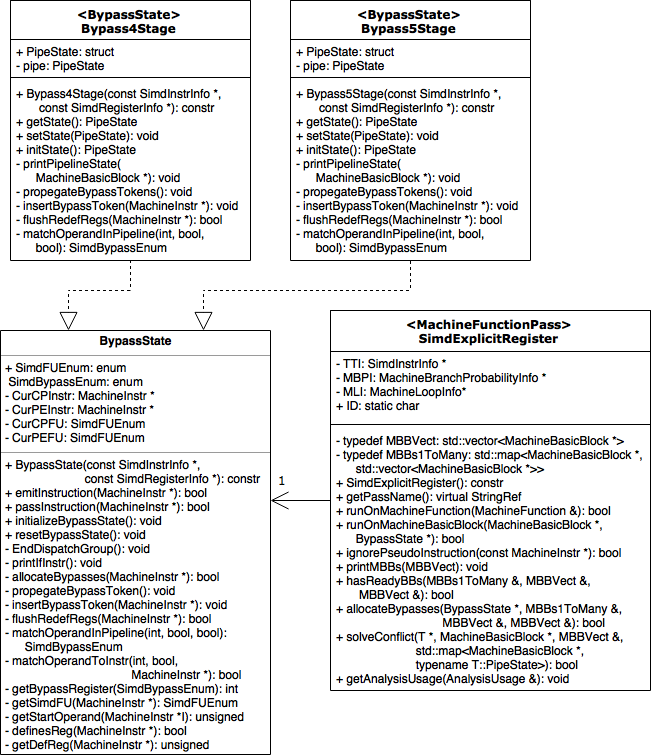
\includegraphics[width=.9\textwidth]{figures/class_diagram}
%\caption{Class diagram of the implemented approach to support explicit datapaths.}
%\label{fig:class_diagram}
%\end{figure}

There is a class called \texttt{BypassState} which should be inherited by each pipeline that we support, e.g. four-stage and five-stage pipeline. It models the values on busses in the bypass network. %It keeps track of values that reside in those busses which keeps track of the . We have This that can be 

\begin{figure}[b!]
\centering
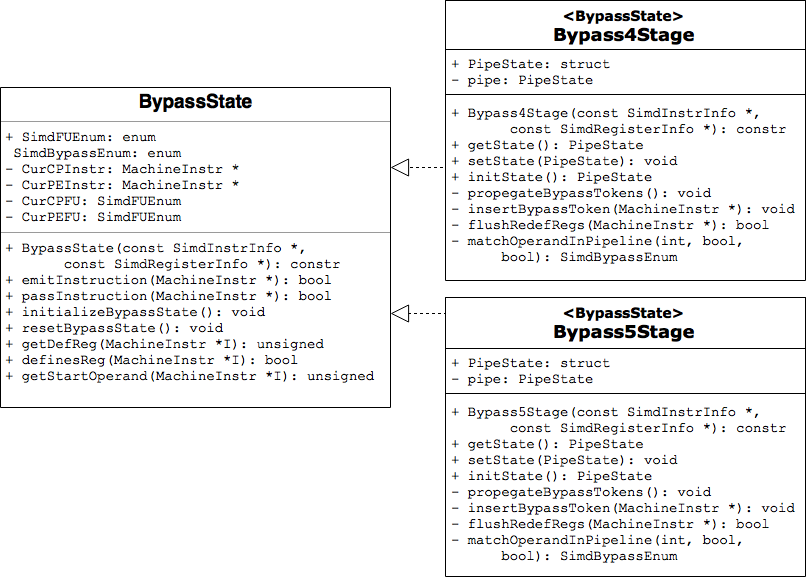
\includegraphics[width=\textwidth]{figures/class_diag_bpstate}
\caption{Class diagram for BypassState, and the inherited classes for the four-stage and five-stage pipelines.}
\label{fig:class_diagram_bpstate}
\end{figure}
%TODO: add following : there was a lot of functionality between the five stage pipeline and four-stage, so we define all shared functionality in \texttt{BypassState}, and stuff specific for a stage in \texttt{BypassXStage}.

We give a class diagram for \texttt{BypassState} in Figure \ref{fig:class_diagram_bpstate}. The classes  \texttt{Bypass4State} and \texttt{Bypass5State} represent the derived classes for the four-stage and five-stage pipeline respectively. Here we use \texttt{insertBypassToken} to pass the instructions in a basic block as tokens to \texttt{BypassState} one at a time and propagate the tokens each cycle using \texttt{propegateBypassTokens}. There is a variable in the derived classes, called \texttt{pipe} which represents the instructions that are currently in our pipeline. The pipeline state can be queried at any giving moment using function \texttt{getState}. This function can be used to acquire the state just before a jump or at the end of a basic block. The functions \texttt{initState} and \texttt{setState} may be used to initialize the state to a empty state, or a given state which is typically done at the beginning of a basic block. We use a function called \texttt{matchOperandInPipeline} to see what bypass can be allocated on a particular use operand of an instruction. It checks whether the operand uses a register defined by any of the instructions the pipeline (by calling \texttt{matchOperandToInstr} and \texttt{getDefReg} for each instruction can be forwarded). In general, it needs to find the newest definition of the register under consideration, therefore, when inserting a bypass token in the pipeline state we remove all occurrences using \texttt{flushRedefRegs}. This way we never have more than one instruction in the pipeline that define the same register, and thus always find the newest definition, if any.

Now lets continue with functions that handle instructions which are used to emit, pass or check an instruction (\texttt{emitInstruction}, \texttt{passInstruction} and \texttt{checkInstruction}). Emitting an instruction consists of the process of specifying which operations are in the current cycle and bypassing their operands according to the current pipeline state. Then pass instruction does the same, but the operands are not bypassed and check instruction does also not actually bypass the operands, but does keep the bypasses that it would allocate in a list. The functions \texttt{allocateBypasses} and \texttt{checkBypasses} do the actual bypassing work by calling \texttt{matchOperandInPipeline} which compares each operand of an instruction to  that can be bypassed. However, there are also flag operands that we do not consider. 
%\lstset{style=customasm}
%TODO: do something cool on the vector slots 
%\vspace{12px}
\begin{lstlisting}
    %loop
        sfgts r2, -64    || v.sfltu   P1, r1, 4
        bf    %loop      || v.slli.P1 r2, r1, 2
        add   r2, r2, -1 || v.add.P1  r7, r6, r2 
    %end:
                         <@\hspace{4px}$\vdots$@>
\end{lstlisting}

%TODO: move next paragraph to above listing, and remove newline
Flag operands occur before register source operands. The code fragment above shows an example of predicate instructions that uses flag operands to either do or not do a certain operation. In this case, we do a shift and add it with something if PE index is smaller than four ($P1$ is true). The function \texttt{getStartOperand} is used to skip flag operands. Alternatively we could also just ignore an operand if it is a flag operand. \\

After each cycle, a call is made to \texttt{EndDispatchGroup} which calls \texttt{insertBypassTokens} for each instruction in the current dispatch (can be two operations, a scalar and a vector op) and propagate the bypass tokens. So to summarize, operands are bypassed when they come across, and at the end of each cycle the pipeline is updated. %Meanwhile using getDef skip all instructions that occur but do not define an instruction. 


%TODO: verify and uncomment
%  later functions do not allocate bypass registers but may be used to insert instructions in the bypass state model, or to check which bypasses would be allocated according to a given bypass state (using \texttt{checkBypasses}), while the first one (\texttt{emitInstruction}) inserts the instruction into the bypass state model and allocates explicit bypasses wherever possible using \texttt{allocateBypasses}.


%TODO: verify and uncomment
% functions \texttt{getDefReg} and \texttt{definesReg} can be used to determine what is written to the register file by an operation, and \texttt{getStartOperand} may be used to see where in an operation we need to start with bypassing RaW dependencies. Function \texttt{matchOperandInPipeline} from the derived classes can be used to see if we can exploit one of the busses in a pipeline. We model these busses with a structure, called \texttt{PipeState}. 

%\begin{table}[b]
%\caption{Representation of struct PipeState.}
%\begin{center}
%\begin{tabular}{@{}l l@{}}
%\toprule
%\textbf{Type} & \textbf{Variable} \\
%MachineInstr* 	& Pipeline[N\_FUNCTION\_UNITS][N\_PACKET\_COUNT][EX\_STAGES]\\
%MachineInstr* 	& WB[N\_PACKET\_COUNT]\\
%SimdFUEnum	& issues[N\_PACKET\_COUNT][EX\_STAGES]\\
%{\small *: pointer}\\
%\bottomrule%%\\
%%{\small * pointer}
%\end{tabular}
%\end{center}
%\label{table:pipe_state}
%\end{table}%
\end{appendices}
%end{appendices}

%\addcontentsline{toc}{chapter}{Appendix A: Supported Operations}
%\appendix
%\addcontentsline{toc}{chapter}{Appendix B}
%\appendix
%\addcontentsline{toc}{chapter}{Appendix C: File Structure}
\end{document}
